% -*- TeX:EN -*-
\documentclass[12pt,twoside,a4paper]{report}
%\documentclass[12pt,twoside,a4paper]{report}
\usepackage{acronym}
\usepackage{pdflscape} % Add this line to import the necessary package
\usepackage{a4}
%\usepackage[ngerman]{babel}    % sorgt für deutsche Überschriften, neue deutsche Rechtschreibung usw.
\usepackage[normal,bf]{caption}    % Formats table and figure captions (see Pdf-file eps-latex p. 51)
\usepackage{graphicx} % to include graphics
%\usepackage{cite}   % to order references, e.g. [12-17] (or use package citesort)
\usepackage{amsmath}    % for ams-tex symbols
\usepackage{amsfonts}
\usepackage{amssymb}
\usepackage{fancyhdr}   % header layout (see Pdf-file fancyhdr)
\usepackage{xspace}     % for empty lines in Mathmode
% \usepackage[ngerman]{babel}
\usepackage[american]{babel}
\usepackage[utf8]{inputenc}

\usepackage{floatflt}
\usepackage{xcolor} % notwendig zur Farbumwandlung für hyperref
\usepackage[pdfborder={0 0 0},citecolor={red}]{hyperref}
\usepackage{listings}
\usepackage{subfigure}
% \usepackage[caption=false, lofdepth=1, lotdepth, margin=5pt]{subfig}
% \usepackage{subcaption}
%\usepackage{subfig}
\usepackage{csquotes}
\usepackage[style=phys,backend=biber,biblabel=brackets]{biblatex}
\addbibresource{bibliography.bib}   % Pfad zu *.bib Dateien für Literaturverzeichnis
% \addbibresource{bibliography.bib}
\usepackage{url}
\urlstyle{same}

\usepackage{makeidx}    % Stichwortverzeichnis
\makeindex

\usepackage{array}

% Glossaries
\usepackage[acronym,indexonlyfirst,nomain]{glossaries}
\renewcommand*{\acronymname}{List of Abbreviations}
\renewcommand*{\glsgroupskip}{}
\makenoidxglossaries

\usepackage{csquotes}
%%%%%%%%%%%%%%%%%%%%%%%%%automatic EPS to PDF conversion(only if eps is newer than pdf%%%%%%%%%%%%%%%%%
\newif\ifpdf
\ifx\pdfoutput\undefined
   \pdffalse
\else
   \pdfoutput=1
   \pdftrue
\fi
\ifpdf
   \usepackage{epstopdf}
   \DeclareGraphicsRule{.eps}{pdf}{.pdf}{`epstopdf #1}
   \pdfcompresslevel=9
\fi
\epstopdfsetup{suffix=}
%%%%%%%%%%%%%%%%%%%%%%%%%%%%%%%%%%%%%%%%%%%%%%%%%%%%%%%%%%%%%%%%%%%%%%%%%%%%%%%%%%%%%%%%%%%%%%%%%%%%%%%%%

%%%%%%%%%%%%%%%%%%%%%%%%%%%%%%Abkürzungsverzeichnis%%%%%%%%%%%%%%%%%%%%%%%%%%%%%%%%%%%%%%%%%%%%%%%%%%%%%%%%%%%%%%%%%%%%%%%
%\usepackage[german]{nomencl} % german macht aus der Überschrift Nomenclature Symbolverzeichnis
%\usepackage{expdlist}
%\renewcommand{\nomname}{Formelzeichen und Abkürzungen}
%\newcommand{\nomunit}[1]{\renewcommand{\nomentryend}{\hspace*{\fill}#1}}
%\makenomenclature % zu Anfang auskommentieren
%Befehl ausführen mit
%(Kopieren und mit rechter Maustaste in Konsole einfügen)
%makeindex  Masterarbeit.nlo -s  nomencl.ist -o Masterarbeit.nls
%Abkürzung für \nomenclature (fz für Formelzeichen)
% \fz{Symbol}{Beschreibung}{Einheit}
%\newcommand{\fz}[3]{\nomenclature{#1}{#2 \nomunit{#3}}}
%
\newacronym{abc}{ABC}{A Basic Concept}
\newacronym{er}{ER}{error rate}
\newacronym{fr}{FR}{Fehlerrate}
\newacronym[plural={RDBMS},shortplural={RDBMS}]{rdbms}{RDBMS}{Relational Database Management System}
\newacronym{vr}{VR}{Virtual Reality}
\newacronym{hri}{HRI}{Human-Robot Interaction}
\newacronym{ear}{EAR}{egocentric action recognition}
\newacronym{vit}{ViT}{Vision Transformer}
\newacronym{dctg}{DCTG}{dynamic class token generator}
\newacronym{padm}{PADM}{Pyramid Architecture with a Dynamic Merging}
\newacronym{fpv}{FPV}{first person view}
\newacronym{hod}{HOD}{Hand and Object Detector}
\newacronym{cnn}{CNNs}{convolutional neural networks}
\newacronym{tsn}{TSN}{Temporal Segment Networks}
\newacronym{tsm}{TSM}{termed temporal shift module}
\newacronym{nlp}{NLP}{natural language processing}
\newacronym{vivit}{ViViT}{Video Vision Transformer}
\newacronym{vst}{}{Video Swin Transformer}
\newacronym{msa}{MSA}{multi-Head Self-Attention}
\newacronym{ffn}{FFN}{feed-forward network}
\newacronym{ln}{LN}{Layer Normalization}
\newacronym{dct}{DCT}{Dynamic Class Token}
\newacronym{gedctg}{GEDCTG}{Gaze-Enhanced Dynamic Class Token Generator}
\newacronym{lstm}{LSTM}{long short-term memory}
%%%%%%%%%%%%%%%%%%%%%%%%%%%%%%%%%%%%%%%%%%%%%%%%%%%%%%%%%%%%%%%%%%%%%%%%%%%%%%%%%%%%%%%%%%%%%%%%%%%%%%%%%%%%%%%%%%%%%%%

%%%%%%%%%%%%%%%%%%%%%%%%%%%%%%%%%%%%%%%%%%%
%  paper format
%%%%%%%%%%%%%%%%%%%%%%%%%%%%%%%%%%%%%%%%%%%
%-----------------------------------------
\setlength{\paperheight}{297mm}
\setlength{\paperwidth}{210mm}
\setlength{\evensidemargin}{5mm}
\setlength{\oddsidemargin}{5mm}
\setlength{\topmargin}{0mm}
\setlength{\footskip}{12mm}
%-----------------------------------------

%%%%%%%%%%%%%%%%%%%%%%%%%%%%%%%%%%%%%%%%%%
% text paragraphs
%%%%%%%%%%%%%%%%%%%%%%%%%%%%%%%%%%%%%%%%%%%
\setlength{\textwidth}{15cm}

%-----------------------------------------
% line spacing
\renewcommand{\baselinestretch}{1.2}
% paragraph indent
\setlength{\parindent}{5mm}
%-----------------------------------------
%
%%%%%%%%%%%%%%%%%%%%%%%%%%%%%%%%%%%%%%%%%%%
%  header and footer
%%%%%%%%%%%%%%%%%%%%%%%%%%%%%%%%%%%%%%%%%%%
%-----------------------------------------

%\clearpage{\pagestyle{empty}\cleardoublepage}   % empty page without header
%-----------------------------------------
%

%%%%%%%%%%%%%%%%%%%%%%%%%%%%%%%%%%%%%%%%%%
%  footnote control and header
%%%%%%%%%%%%%%%%%%%%%%%%%%%%%%%%%%%%%%%%%%%
%-----------------------------------------
\pagestyle{fancy}
\fancyhf{} % clear all fields
\fancyhead[LE,RO]{\thepage}        % E and O are Even and Odd pages, L, R and C stand for
                                    % Left, Right und Center
\fancyhead[RE]{\slshape \leftmark} % \leftmark (higher level, e.g. chapter) is first
                                    % argument of \markboth{}{},
                                    % \rightmark (lower level, e.g. section) second %argument (or  argument of \markright{})
\fancyhead[LO]{\slshape \rightmark} % \fancyfoot[LE,RO]{\thepage}
\renewcommand{\chaptermark}[1]{\markboth{\MakeUppercase{\chaptername\ \thechapter.\ #1}}{}} % \chaptername=name of chapter \thechapter=Number of chapter Argument #1 is the
        % name of the chapter
\renewcommand{\sectionmark}[1]{\markright{\MakeUppercase{\thesection\ #1}}}
\renewcommand{\headheight}{1.5cm}
\renewcommand{\headrulewidth}{0.4pt}
\renewcommand{\footrulewidth}{0.4pt}

%%%%%%%%%%%%%%%%%%%%%%%%%%%%%%%%%%%%%%%%%%%
%  settings for float environments such as figures
%%%%%%%%%%%%%%%%%%%%%%%%%%%%%%%%%%%%%%%%%%%
%-----------------------------------------
% page layout
\setcounter{topnumber}{2}     % Maximum number of floats at the top of a page
\setcounter{bottomnumber}{2}  % Maximum number of floats at the bottom of a page
\setcounter{totalnumber}{4}   % Maximum number of floats on a page
\renewcommand{\topfraction}{1}     %
\renewcommand{\bottomfraction}{1}  %
\renewcommand{\textfraction}{0.05} % minimal fraction of text on a page
\renewcommand{\floatpagefraction}{0.7}  %minimal fraction of floats on a pure float page
%-----------------------------------------
% distances to float objects
\setlength{\floatsep}{0pt}      % spaces at top and bottom of a page
\setlength{\textfloatsep}{0ex}  % spaces to text
\setlength{\intextsep}{0ex}     % spaces in text
%-----------------------------------------
%

%%%%%%%%%%%%%%%%%%%%%%%
% Table and figure captions
% see usepackage caption2
%%%%%%%%%%%%%%%%%%%%%%%
%\addto\captionsenglish{%
%\renewcommand\chaptername{Kapitel}}
%\renewcommand{\chaptername}{Kapitel}
\renewcommand{\figurename}{Bild}
\addto\captionsngerman{\renewcommand{\figurename}{Bild}}
\renewcommand{\tablename}{Tab.}




%\addto\captionsngerman{\renewcommand{\listfigurename}{Bildverzeichnis}}


%\renewcaptionname{ngerman}{\listfigurename}{Bildverzeichnis}

% \mycaption{Table or Figure caption}{entry for the list of tables / figures}
\newcommand{\mycaption}[2]{\caption[#2]{\tss{#1}}}

% Trennungshilfe
\hyphenation{Se-lek-tion Mak-ro-zel-le}


%%%%%%%%%%%%%%%%%%
% directory for figures
%%%%%%%%%%%%%%%%%%%%
\makeatletter
\def\input@path{{figures/}{figures/figures2/}{figures/grafiken/}}
\makeatother %  definiert in welchen Verzeichnissen bei Aufruf von /input gesucht werden soll, notwenig für \includesvg

\graphicspath{{figures/}{figures/figures2/}{figures/grafiken}}    % defines the path where latex looks for figures
% %\documentclass[12pt,twoside,a4paper]{report}
\usepackage{acronym}
\usepackage{pdflscape} % Add this line to import the necessary package
\usepackage{a4}
%\usepackage[ngerman]{babel}    % sorgt für deutsche Überschriften, neue deutsche Rechtschreibung usw.
\usepackage[normal,bf]{caption}    % Formats table and figure captions (see Pdf-file eps-latex p. 51)
\usepackage{graphicx} % to include graphics
%\usepackage{cite}   % to order references, e.g. [12-17] (or use package citesort)
\usepackage{amsmath}    % for ams-tex symbols
\usepackage{amsfonts}
\usepackage{amssymb}
\usepackage{fancyhdr}   % header layout (see Pdf-file fancyhdr)
\usepackage{xspace}     % for empty lines in Mathmode
% \usepackage[ngerman]{babel}
\usepackage[american]{babel}
\usepackage[utf8]{inputenc}

\usepackage{floatflt}
\usepackage{xcolor} % notwendig zur Farbumwandlung für hyperref
\usepackage[pdfborder={0 0 0},citecolor={red}]{hyperref}
\usepackage{listings}
\usepackage{subfigure}
% \usepackage[caption=false, lofdepth=1, lotdepth, margin=5pt]{subfig}
% \usepackage{subcaption}
%\usepackage{subfig}
\usepackage{csquotes}
\usepackage[style=phys,backend=biber,biblabel=brackets]{biblatex}
\addbibresource{bibliography.bib}   % Pfad zu *.bib Dateien für Literaturverzeichnis
% \addbibresource{bibliography.bib}
\usepackage{url}
\urlstyle{same}

\usepackage{makeidx}    % Stichwortverzeichnis
\makeindex

\usepackage{array}

% Glossaries
\usepackage[acronym,indexonlyfirst,nomain]{glossaries}
\renewcommand*{\acronymname}{List of Abbreviations}
\renewcommand*{\glsgroupskip}{}
\makenoidxglossaries

\usepackage{csquotes}
%%%%%%%%%%%%%%%%%%%%%%%%%automatic EPS to PDF conversion(only if eps is newer than pdf%%%%%%%%%%%%%%%%%
\newif\ifpdf
\ifx\pdfoutput\undefined
   \pdffalse
\else
   \pdfoutput=1
   \pdftrue
\fi
\ifpdf
   \usepackage{epstopdf}
   \DeclareGraphicsRule{.eps}{pdf}{.pdf}{`epstopdf #1}
   \pdfcompresslevel=9
\fi
\epstopdfsetup{suffix=}
%%%%%%%%%%%%%%%%%%%%%%%%%%%%%%%%%%%%%%%%%%%%%%%%%%%%%%%%%%%%%%%%%%%%%%%%%%%%%%%%%%%%%%%%%%%%%%%%%%%%%%%%%

%%%%%%%%%%%%%%%%%%%%%%%%%%%%%%Abkürzungsverzeichnis%%%%%%%%%%%%%%%%%%%%%%%%%%%%%%%%%%%%%%%%%%%%%%%%%%%%%%%%%%%%%%%%%%%%%%%
%\usepackage[german]{nomencl} % german macht aus der Überschrift Nomenclature Symbolverzeichnis
%\usepackage{expdlist}
%\renewcommand{\nomname}{Formelzeichen und Abkürzungen}
%\newcommand{\nomunit}[1]{\renewcommand{\nomentryend}{\hspace*{\fill}#1}}
%\makenomenclature % zu Anfang auskommentieren
%Befehl ausführen mit
%(Kopieren und mit rechter Maustaste in Konsole einfügen)
%makeindex  Masterarbeit.nlo -s  nomencl.ist -o Masterarbeit.nls
%Abkürzung für \nomenclature (fz für Formelzeichen)
% \fz{Symbol}{Beschreibung}{Einheit}
%\newcommand{\fz}[3]{\nomenclature{#1}{#2 \nomunit{#3}}}
%
\newacronym{abc}{ABC}{A Basic Concept}
\newacronym{er}{ER}{error rate}
\newacronym{fr}{FR}{Fehlerrate}
\newacronym[plural={RDBMS},shortplural={RDBMS}]{rdbms}{RDBMS}{Relational Database Management System}
\newacronym{vr}{VR}{Virtual Reality}
\newacronym{hri}{HRI}{Human-Robot Interaction}
\newacronym{ear}{EAR}{egocentric action recognition}
\newacronym{vit}{ViT}{Vision Transformer}
\newacronym{dctg}{DCTG}{dynamic class token generator}
\newacronym{padm}{PADM}{Pyramid Architecture with a Dynamic Merging}
\newacronym{fpv}{FPV}{first person view}
\newacronym{hod}{HOD}{Hand and Object Detector}
\newacronym{cnn}{CNNs}{convolutional neural networks}
\newacronym{tsn}{TSN}{Temporal Segment Networks}
\newacronym{tsm}{TSM}{termed temporal shift module}
\newacronym{nlp}{NLP}{natural language processing}
\newacronym{vivit}{ViViT}{Video Vision Transformer}
\newacronym{vst}{}{Video Swin Transformer}
\newacronym{msa}{MSA}{multi-Head Self-Attention}
\newacronym{ffn}{FFN}{feed-forward network}
\newacronym{ln}{LN}{Layer Normalization}
\newacronym{dct}{DCT}{Dynamic Class Token}
\newacronym{gedctg}{GEDCTG}{Gaze-Enhanced Dynamic Class Token Generator}
\newacronym{lstm}{LSTM}{long short-term memory}
%%%%%%%%%%%%%%%%%%%%%%%%%%%%%%%%%%%%%%%%%%%%%%%%%%%%%%%%%%%%%%%%%%%%%%%%%%%%%%%%%%%%%%%%%%%%%%%%%%%%%%%%%%%%%%%%%%%%%%%

%%%%%%%%%%%%%%%%%%%%%%%%%%%%%%%%%%%%%%%%%%%
%  paper format
%%%%%%%%%%%%%%%%%%%%%%%%%%%%%%%%%%%%%%%%%%%
%-----------------------------------------
\setlength{\paperheight}{297mm}
\setlength{\paperwidth}{210mm}
\setlength{\evensidemargin}{5mm}
\setlength{\oddsidemargin}{5mm}
\setlength{\topmargin}{0mm}
\setlength{\footskip}{12mm}
%-----------------------------------------

%%%%%%%%%%%%%%%%%%%%%%%%%%%%%%%%%%%%%%%%%%
% text paragraphs
%%%%%%%%%%%%%%%%%%%%%%%%%%%%%%%%%%%%%%%%%%%
\setlength{\textwidth}{15cm}

%-----------------------------------------
% line spacing
\renewcommand{\baselinestretch}{1.2}
% paragraph indent
\setlength{\parindent}{5mm}
%-----------------------------------------
%
%%%%%%%%%%%%%%%%%%%%%%%%%%%%%%%%%%%%%%%%%%%
%  header and footer
%%%%%%%%%%%%%%%%%%%%%%%%%%%%%%%%%%%%%%%%%%%
%-----------------------------------------

%\clearpage{\pagestyle{empty}\cleardoublepage}   % empty page without header
%-----------------------------------------
%

%%%%%%%%%%%%%%%%%%%%%%%%%%%%%%%%%%%%%%%%%%
%  footnote control and header
%%%%%%%%%%%%%%%%%%%%%%%%%%%%%%%%%%%%%%%%%%%
%-----------------------------------------
\pagestyle{fancy}
\fancyhf{} % clear all fields
\fancyhead[LE,RO]{\thepage}        % E and O are Even and Odd pages, L, R and C stand for
                                    % Left, Right und Center
\fancyhead[RE]{\slshape \leftmark} % \leftmark (higher level, e.g. chapter) is first
                                    % argument of \markboth{}{},
                                    % \rightmark (lower level, e.g. section) second %argument (or  argument of \markright{})
\fancyhead[LO]{\slshape \rightmark} % \fancyfoot[LE,RO]{\thepage}
\renewcommand{\chaptermark}[1]{\markboth{\MakeUppercase{\chaptername\ \thechapter.\ #1}}{}} % \chaptername=name of chapter \thechapter=Number of chapter Argument #1 is the
        % name of the chapter
\renewcommand{\sectionmark}[1]{\markright{\MakeUppercase{\thesection\ #1}}}
\renewcommand{\headheight}{1.5cm}
\renewcommand{\headrulewidth}{0.4pt}
\renewcommand{\footrulewidth}{0.4pt}

%%%%%%%%%%%%%%%%%%%%%%%%%%%%%%%%%%%%%%%%%%%
%  settings for float environments such as figures
%%%%%%%%%%%%%%%%%%%%%%%%%%%%%%%%%%%%%%%%%%%
%-----------------------------------------
% page layout
\setcounter{topnumber}{2}     % Maximum number of floats at the top of a page
\setcounter{bottomnumber}{2}  % Maximum number of floats at the bottom of a page
\setcounter{totalnumber}{4}   % Maximum number of floats on a page
\renewcommand{\topfraction}{1}     %
\renewcommand{\bottomfraction}{1}  %
\renewcommand{\textfraction}{0.05} % minimal fraction of text on a page
\renewcommand{\floatpagefraction}{0.7}  %minimal fraction of floats on a pure float page
%-----------------------------------------
% distances to float objects
\setlength{\floatsep}{0pt}      % spaces at top and bottom of a page
\setlength{\textfloatsep}{0ex}  % spaces to text
\setlength{\intextsep}{0ex}     % spaces in text
%-----------------------------------------
%

%%%%%%%%%%%%%%%%%%%%%%%
% Table and figure captions
% see usepackage caption2
%%%%%%%%%%%%%%%%%%%%%%%
%\addto\captionsenglish{%
%\renewcommand\chaptername{Kapitel}}
%\renewcommand{\chaptername}{Kapitel}
\renewcommand{\figurename}{Bild}
\addto\captionsngerman{\renewcommand{\figurename}{Bild}}
\renewcommand{\tablename}{Tab.}




%\addto\captionsngerman{\renewcommand{\listfigurename}{Bildverzeichnis}}


%\renewcaptionname{ngerman}{\listfigurename}{Bildverzeichnis}

% \mycaption{Table or Figure caption}{entry for the list of tables / figures}
\newcommand{\mycaption}[2]{\caption[#2]{\tss{#1}}}

% Trennungshilfe
\hyphenation{Se-lek-tion Mak-ro-zel-le}


%%%%%%%%%%%%%%%%%%
% directory for figures
%%%%%%%%%%%%%%%%%%%%
\makeatletter
\def\input@path{{figures/}{figures/figures2/}{figures/grafiken/}}
\makeatother %  definiert in welchen Verzeichnissen bei Aufruf von /input gesucht werden soll, notwenig für \includesvg

\graphicspath{{figures/}{figures/figures2/}{figures/grafiken}}    % defines the path where latex looks for figures	% Pakete und Konfiguration

% % Custom commands and configurations
%
\newacronym{abc}{ABC}{A Basic Concept}
\newacronym{er}{ER}{error rate}
\newacronym{fr}{FR}{Fehlerrate}
\newacronym[plural={RDBMS},shortplural={RDBMS}]{rdbms}{RDBMS}{Relational Database Management System}
\newacronym{vr}{VR}{Virtual Reality}
\newacronym{hri}{HRI}{Human-Robot Interaction}
\newacronym{ear}{EAR}{egocentric action recognition}
\newacronym{vit}{ViT}{Vision Transformer}
\newacronym{dctg}{DCTG}{dynamic class token generator}
\newacronym{padm}{PADM}{Pyramid Architecture with a Dynamic Merging}
\newacronym{fpv}{FPV}{first person view}
\newacronym{hod}{HOD}{Hand and Object Detector}
\newacronym{cnn}{CNNs}{convolutional neural networks}
\newacronym{tsn}{TSN}{Temporal Segment Networks}
\newacronym{tsm}{TSM}{termed temporal shift module}
\newacronym{nlp}{NLP}{natural language processing}
\newacronym{vivit}{ViViT}{Video Vision Transformer}
\newacronym{vst}{}{Video Swin Transformer}
\newacronym{msa}{MSA}{multi-Head Self-Attention}
\newacronym{ffn}{FFN}{feed-forward network}
\newacronym{ln}{LN}{Layer Normalization}
\newacronym{dct}{DCT}{Dynamic Class Token}
\newacronym{gedctg}{GEDCTG}{Gaze-Enhanced Dynamic Class Token Generator}
\newacronym{lstm}{LSTM}{long short-term memory} % Include the glossary definitions

\newacronym{abc}{ABC}{A Basic Concept}
\newacronym{er}{ER}{error rate}
\newacronym{fr}{FR}{Fehlerrate}
\newacronym[plural={RDBMS},shortplural={RDBMS}]{rdbms}{RDBMS}{Relational Database Management System}
\newacronym{vr}{VR}{Virtual Reality}
\newacronym{hri}{HRI}{Human-Robot Interaction}
\newacronym{ear}{EAR}{egocentric action recognition}
\newacronym{vit}{ViT}{Vision Transformer}
\newacronym{dctg}{DCTG}{dynamic class token generator}
\newacronym{padm}{PADM}{Pyramid Architecture with a Dynamic Merging}
\newacronym{fpv}{FPV}{first person view}
\newacronym{hod}{HOD}{Hand and Object Detector}
\newacronym{cnn}{CNNs}{convolutional neural networks}
\newacronym{tsn}{TSN}{Temporal Segment Networks}
\newacronym{tsm}{TSM}{termed temporal shift module}
\newacronym{nlp}{NLP}{natural language processing}
\newacronym{vivit}{ViViT}{Video Vision Transformer}
\newacronym{vst}{}{Video Swin Transformer}
\newacronym{msa}{MSA}{multi-Head Self-Attention}
\newacronym{ffn}{FFN}{feed-forward network}
\newacronym{ln}{LN}{Layer Normalization}
\newacronym{dct}{DCT}{Dynamic Class Token}
\newacronym{gedctg}{GEDCTG}{Gaze-Enhanced Dynamic Class Token Generator}
\newacronym{lstm}{LSTM}{long short-term memory}
%%%%%%%%%%%%%%%%%%%%%%%%%%%%%%%%%%%%%%%%%%%%%%%%%%%%%%%%%%%%%%%%%%%%%%%%%%
\begin{document}

% Titelseite 
%Inhaltsverzeichnis
%%%%%%%%%%%%%%%%%%%%%%%%%%%%%%%%%%%%%%%%%%%%%%%%%%%%%%%%%%%%%%%%%%%%%%%
%Titelblatt
%%%%%%%%%%%%%%%%%%%%%%%%%%%%%%%%%%%%%%%%%%%%%%%%%%%%%%%%%%%%%%%%%%%%%%%
\thispagestyle{empty}

\enlargethispage{25mm}

%%%%%%%%%%%%%%%%%%%%%%%%%uni logo%%%%%%%%%%%%%%%%%%%%%%%%%
\vspace*{-30mm}

\includegraphics[width=100mm]{uni-stuttgart-logo.eps}


\begin{center}
\vspace{10mm}



\includegraphics[width=130mm]{ipv_logo_2011Masterarbeit.pdf}

\vspace{15mm} \Large{\bf Gaze-based Transformer for Improving Action Recognition in Egocentric Videos}  %%Titel der Arbeit

\vspace{15mm} \large
Master Thesis\\
Mengze Lu


\vspace{6mm} 15.01.2024 - 15.07.2024 %Bearbeitungszeitraum

\vspace{6mm} Supervisor: Dr. Lei Shi \\
\vspace{3mm} Second Examiner: Prof. Dr. Andreas Bulling

\vspace{6mm}
Prof. Dr.-Ing. Kai Peter Birke\\
Fachgebiet Elektrische Energiespeichersysteme (EES)\\
Institut für Photovoltaik\\

Pfaffenwaldring 47\\
{D-70569 Stuttgart}\\


\end{center}

\clearpage{\pagestyle{empty}\cleardoublepage}   %Leerseiten ohne Kopfzeile

%%%%%%%%%%%%%%%%%%%%%%%%%%%%%%%%%%%%%%%%%%%%%%%%%%%%%%%%%%%%%%%%%%%%%%%%%%%%%%

%%%%%%%%%%%%%%%%%%%%%%%%%%%%%%%%%%%%%%%%%%%%%%%%%%%%%%%%%%%%%%%%%%%%%%%%%%%%%%
%Inhaltsverzeichnis
%%%%%%%%%%%%%%%%%%%%%%%%%%%%%%%%%%%%%%%%%%%%%%%%%%%%%%%%%%%%%%%%%%%%%%%%%%%%%%

\pagenumbering{roman} % oder Roman ? (Römische Seitenzahlen)
\setcounter{page}{1}

%Tiefe der Eintr�ge im Inhaltsverzeichnis (0 chapter, 1 section, 2 subsection...)
\setcounter{tocdepth}{2}

%Inhaltsverzeichnis
\tableofcontents

\clearpage{\pagestyle{empty}\cleardoublepage}   %Leerseiten ohne Kopfzeile



%Tiefe der Abschnittsnumerierung
\setcounter{secnumdepth}{2}

\rm\normalsize \pagenumbering{arabic} \setcounter{page}{1}
%%%%%%%%%%%%%%%%%%%%%%%%%%%%%%%%%%%%%%%%%%%%%%%%%%%%%%%%%%%%%%%%%%%%%%%%%%%%%%%%%
\newcommand{\latex}{\LaTeX}
\newcommand{\biblatex}{Bib\LaTeX}
\newcommand{\tab}[1]{Tabelle \ref{tab:#1}}
\newcommand{\Egquer}{{\bar{E}_{ \mathrm{g}}}}
\newcommand{\sigmaEg}{{\sigma_{ \mathrm{Eg}}}}
\newcommand{\fig}[1]{Bild \ref{fig:#1}}
% Einheiten
\newcommand{\mJ}{\unit{mJ}}
\newcommand{\kV}{\unit{kV}}
\newcommand{\mAh}{\unit{mAh}}
\newcommand{\g}{\unit{g}}
\newcommand{\As}{\unit{As}}
\newcommand{\mol}{\unit{mol}}
\newcommand{\mA}{\unit{mA}}
\newcommand{\kB}{{k_{ \mathrm{ B}}}}
\newcommand{\m}{\unit{m}}
\newcommand{\J}{\unit{J}}
\newcommand{\mbar}{\unit{mbar}}
\newcommand{\unit}[1]{{\,\rm #1}} %Einheiten (Aufrecht)
\newcommand{\A}{\unit{A}}
\newcommand{\Celsius}{\unit{^\circ C}}
\newcommand{\cm}{\unit{cm}}
\newcommand{\dB}{\unit{dB}} %deziBel
\newcommand{\Dekade}{\unit{Dec}} %Dekade
\newcommand{\eV}{\unit{eV}}
\newcommand{\eVolt}{\unit{eV}}
\newcommand{\Farad}{\unit{F}}
\newcommand{\GHz}{\unit{GHz}}
\newcommand{\Hz}{\unit{Hz}}
\newcommand{\inch}{\unit{inch}} %Ein Zoll
\newcommand{\K}{\unit{K}}
\newcommand{\kHz}{\unit{kHz}}
\newcommand{\meV}{\unit{meV}}
\newcommand{\MHz}{\unit{MHz}}
\newcommand{\mm}{\unit{mm}}
\newcommand{\mSek}{\unit{ms}} %Millisekunde
\newcommand{\mum}{\unit{\mu m}}
\newcommand{\muSek}{\unit{\mu s}} %Mikrosekunde
\newcommand{\mTorr}{\unit{mTorr}}
\newcommand{\mV}{\unit{mV}}
\newcommand{\mVolt}{\unit{mV}}
\newcommand{\mW}{\unit{mW}}
\newcommand{\nF}{\unit{nF}} %Nanno Farrad
\newcommand{\nH}{\unit{nH}} %Nanno Henry
\newcommand{\nm}{\unit{nm}}
\newcommand{\nSek}{\unit{ns}} %Nanosekunde
\newcommand{\Ohm}{\Omega}
\newcommand{\percent}{\unit{\%}}
\newcommand{\pF}{\unit{pF}} %Pico Farrad
\newcommand{\pH}{\unit{pH}} %Pico Henry
\newcommand{\pSek}{\unit{ps}} %Picosekunde
\newcommand{\s}{\unit{s}} %Sekunde
\newcommand{\V}{\unit{V}}
\newcommand{\W}{\unit{W}}
\renewcommand{\min}{\unit{min}} %Sekunde
\newcommand{\keV}{\unit{keV}}
\newcommand{\h}{\unit{h}}
\newcommand{\sq}{\unit{sq}}
\newcommand{\pA}{\unit{pA}}
\newcommand{\nA}{\unit{nA}}
\newcommand{\Ah}{\unit{Ah}}
\newcommand{\kOhm}{\unit{k\Omega}}

% Schriftgroessen im Math-Modus
%
\newcommand{\TS}{\textstyle}
\newcommand{\DS}{\displaystyle}
\newcommand{\SCS}{\scriptstyle}
\newcommand{\SCSCS}{\scriptscriptstyle}
%
%
% Schriftarten im Math-Modus
%
\newcommand{\kuno}[1]{$#1$}                  %kursiv, normal
\newcommand{\upno}[1]{\mbox{\rm{#1}}}        %upright(senkrecht), bold
\newcommand{\kubo}[1]{\mbox{\boldmath $#1$}} %kursiv, bold
\newcommand{\upbo}[1]{\mbox{\rm\bf{#1}}}     %upright(senkrecht), bold
%
%%%%%%%%%%%%%%%%%%%%%%%%%%%%%%%%%%%%%%%%%%%%%%%%%%%%%%%%%%%%%%%%%%%%%%%
%Gleichungen und Formeln
%%%%%%%%%%%%%%%%%%%%%%%%%%%%%%%%%%%%%%%%%%%%%%%%%%%%%%%%%%%%%%%%%%%%%%%
\newcommand{\eqn}[2]{\begin{equation}
#1
\label{eqn:#2}
\end{equation}}
%%%%%%%%%%%%%%%%%%%%%%%%%%%%%%%%%%%%%%%%%%%%%%%%%%%%%%%%%%%%%%%%%%%%%%%


%***********************************************************************%
%
% Schriftgroesse fuer xfig-bilder
%
%***********************************************************************%
%
\newcommand{\tsl}[1]{\large #1}
\newcommand{\tsn}[1]{\normalsize #1}
\newcommand{\tss}[1]{\small #1}
%\newcommand{\tsl}[1]{\Large #1}
%\newcommand{\tsn}[1]{\large #1}
%\newcommand{\tss}[1]{\normalsize #1}
\newcommand{\fsl}[1]{\tsl{$#1$}}
\newcommand{\fsn}[1]{\tsn{$#1$}}
\newcommand{\fss}[1]{\tss{$#1$}}
%


%%%%%%%%%%%%%%%%%%%%%%%%%%%%%%%%%%%%%%%%%%%%%%%%%%%%%%%%%%%%%%%%%%%%%%%%%%%
%
%Tabellen nicht als Abkürzung sondern zum Rauskopieren
%
%%%%%%%%%%%%%%%%%%%%%%%%%%%%%%%%%%%%%%%%%%%%%%%%%%%%%%%%%%%%%%%%%%%%%%%%%%%

%\begin{table}[h!tbp]
%\mycaption{Verdammt wichtige physikalische Konstanten}{}
%\vspace{5mm}
%  \centering
%  \begin{tabular}{ l l }
%    \hline
%    \hline
%    % after \\: \hline or \cline{col1-col2} \cline{col3-col4} ...
%    Größe & Wert \\
%    \hline
%    $q$ &      $1.6 \times 10^{-19} \A\s $ \\
%   $\varepsilon_0 $ &  $ 8.85 \times 10^{-14} \A\s/\V\cm$ \\
%    \hline
%    \hline
%  \end{tabular}
%\vspace{5mm}
%\label{tab:physkonst}
%\end{table}


%***********************************************************************%
%
% Bilder, Rahmen
%
%***********************************************************************%
%\includeps{Breite in Zentimetern 'cm'}{bild_datei}{Unterschrift}{Eintrag ins Abbildungsverzeichnis}
\newcommand{\includeps}[4]{
\begin{figure}[h!tbp]
\vspace{3mm}
  \begin{center}
       \includegraphics[width=#1]{#2.eps}
 \mycaption{#3}{#4}
    \label{fig:#2}
  \end{center}
\vspace{5mm}
\end{figure}
}%
%% Einbinden von PDFs als Bilder
\newcommand{\includepdf}[4]{
\begin{figure}[h!tbp]
\vspace{3mm}
  \begin{center}
       \includegraphics[width=#1]{#2.pdf}
 \mycaption{#3}{#4}
    \label{fig:#2}
  \end{center}
\vspace{5mm}
\end{figure}
}%

%%%  Einbinden von svg's aus inkscape (mit Latexschrift in Bild)
\newcommand{\executeiffilenewer}[3]{%
\ifnum\pdfstrcmp{\pdffilemoddate{#1}}%
{\pdffilemoddate{#2}}>0%
{\immediate\write18{#3}}\fi%
}

\newcommand{\includesvg}[4]{
\begin{figure}[h!tbp]
\vspace{3mm}
  \begin{center}
   \def\svgwidth{#1}
   \executeiffilenewer{#2.svg}{#2.pdf}%
	{inkscape -z -D --file=#2.svg %
	--export-pdf=#2.pdf --export-latex}%
	\input{#2.pdf_tex}
	 \mycaption{#3}{#4}
	    \label{fig:#2}
	  \end{center}
	\vspace{5mm}
	\end{figure}
}
%%%Die folgenden beiden Befehle sind nur für xfig Benutzer relevant
%%Optionen zum Aufruf von xfig, damit der Export von pstex-Grafiken gut funktioniert:
%%xfig -metric -right -but_per_row 3 -portrait -zoom 2 -pheight 18 -pwidth 24 -latexfonts -specialtext -startgridmode 1 -exportL pstex
%%Oder als alias einrichten: z. B.
%%alias lafig 'xfig -metric -right -but_per_row 3 -portrait -zoom 2 -pheight 18 -pwidth 24 -latexfonts -specialtext -startgridmode 1 -exportL pstex'  # xfig fuer latex
%
%%\includepstex{bild_datei}{Unterschrift}{Eintrag ins Abbildungsverzeichnis}
%\newcommand{\includepstex}[3]{
%\begin{figure}[h!tbp]
%\vspace{5mm}
%  \begin{center}
%    %\figbox{ \input{#1.pstex_t} }
%    \input{#1.pstex_t}
%   \mycaption{#2}{#3}
%    \label{fig:#1}
%    \vspace{3mm}
%  \end{center}
%\end{figure}
%}%

%
%%\includepstexshift{bild_datei}{Unterschrift}{H-Shift}{eintrag ins Abbildungsverzeichnis}
%\newcommand{\includepstexshift}[4]{
%\begin{figure}[h!tbp]
%  \begin{center}
%    \figbox{ \hspace*{#3}\input{#1.pstex_t} }
%    \mycaption{#2}{#4}
%    \label{fig:#1}
%  \end{center}
%\end{figure}}%


% Zusammenfassung (Summary)
\chapter*{Abstract}
\addcontentsline{toc}{chapter}{Abstract}
This thesis investigates the integration of gaze information into a transformer-based model to enhance action recognition in egocentric videos. The study focuses on enhancing the \acrlong{dctg} module with additional gaze information.
% within EgoViT, which currently includes a \acrlong{hod} that extracts features from hand-object interactions in video frames. 
The proposed Gaze-Enhanced \gls{dctg} module fuses gaze features with hand-object features to create comprehensive gaze-hand-object features. These features generate a specialized class token that, along with the video frames, guides the transformer to focus on action-related segments. 
% Transformer-based architectures showing promising results for action recognition task in videos. 
The proposed model maintains a similar architecture to the original EgoViT, handing the temporal relationships between short-term phases effectively. A modified Video Swin Transformer serves as the backbone for processing local spatial relationships.

The EGTEA Gaze+ dataset is used for model training and testing. A series of experiments evaluates the impact of gaze information on EAR accuracy. The key objectives are to propose a novel Gaze Extrator module, which generates gaze-box image from input gaze points, and then fed them into a swquential convolutional networks to obtain the gaze features. Results demonstrate that the Gaze-Enhanced EgoViT model achieves a top-1 accuracy of 52.0\% and a top-5 accuracy of 76.3\%, surpassing the baseline EgoViT model. Higher quality gaze features significantly improve performance, with experiments showing that gaze information alone yields a top-1 accuracy above 50\%. These findings highlight the potential of the Gaze-Enhanced EgoViT model to advance action recognition in egocentric videos and suggest further exploration into the role of gaze information in enhancing EAR accuracy.


% This thesis introduces a Gaze-Enhanced \acrlong{dctg} module integrated into the EgoViT model to enhance action recognition in egocentric videos. The Gaze-Enhanced DCTG module focuses on regions of interest in video frames identified through gaze tracking points, detected hands, and objects. By incorporating gaze tracking as an additional input, the model extracts gaze features and merges them with hand-object features from a modified \acrlong{hod} module, generating dynamic class tokens that guide the model's attention. The proposed model maintains a similar architecture to the original EgoViT, handing the temporal relationships between short-term phases effectively. A modified Video Swin Transformer serves as the backbone for processing local spatial relationships. The proposed model was evaluated on the EGTEA Gaze+ dataset, which includes gaze tracking points. The proposed model's performance, notably improved with higher quality gaze features (Gaze version 2), underscores the significant impact of gaze feature quality. Experiments also indicated that the model, using only gaze features, confirming the utility of gaze information in action recognition for egocentric videos. These findings suggest the proposed Gaze-Enhanced EgoViT model as a promising approach for enhancing action recognition in egocentric videos and warrant further investigation into the impact of gaze information on \acrlong{ear}.

% Kapitel %%%%%%%%%%%%%%%%%%%%%%%%%%%%%%%%%%%%%%%%

% This thesis investigates the integration of gaze information into a transformer-based model to enhance action recognition in egocentric videos. The study focuses on enhancing the \acrlong{dctg} module with additional gaze information.
% within EgoViT, which currently includes a \acrlong{hod} that extracts features from hand-object interactions in video frames. 
The proposed Gaze-Enhanced \gls{dctg} module fuses gaze features with hand-object features to create comprehensive gaze-hand-object features. These features generate a specialized class token that, along with the video frames, guides the transformer to focus on action-related segments. 
% Transformer-based architectures showing promising results for action recognition task in videos. 
The proposed model maintains a similar architecture to the original EgoViT, handing the temporal relationships between short-term phases effectively. A modified Video Swin Transformer serves as the backbone for processing local spatial relationships.

The EGTEA Gaze+ dataset is used for model training and testing. A series of experiments evaluates the impact of gaze information on EAR accuracy. The key objectives are to propose a novel Gaze Extrator module, which generates gaze-box image from input gaze points, and then fed them into a swquential convolutional networks to obtain the gaze features. Results demonstrate that the Gaze-Enhanced EgoViT model achieves a top-1 accuracy of 52.0\% and a top-5 accuracy of 76.3\%, surpassing the baseline EgoViT model. Higher quality gaze features significantly improve performance, with experiments showing that gaze information alone yields a top-1 accuracy above 50\%. These findings highlight the potential of the Gaze-Enhanced EgoViT model to advance action recognition in egocentric videos and suggest further exploration into the role of gaze information in enhancing EAR accuracy.


% This thesis introduces a Gaze-Enhanced \acrlong{dctg} module integrated into the EgoViT model to enhance action recognition in egocentric videos. The Gaze-Enhanced DCTG module focuses on regions of interest in video frames identified through gaze tracking points, detected hands, and objects. By incorporating gaze tracking as an additional input, the model extracts gaze features and merges them with hand-object features from a modified \acrlong{hod} module, generating dynamic class tokens that guide the model's attention. The proposed model maintains a similar architecture to the original EgoViT, handing the temporal relationships between short-term phases effectively. A modified Video Swin Transformer serves as the backbone for processing local spatial relationships. The proposed model was evaluated on the EGTEA Gaze+ dataset, which includes gaze tracking points. The proposed model's performance, notably improved with higher quality gaze features (Gaze version 2), underscores the significant impact of gaze feature quality. Experiments also indicated that the model, using only gaze features, confirming the utility of gaze information in action recognition for egocentric videos. These findings suggest the proposed Gaze-Enhanced EgoViT model as a promising approach for enhancing action recognition in egocentric videos and warrant further investigation into the impact of gaze information on \acrlong{ear}.
% \include{chapters/Warumtex}
% \include{chapters/ipetex}
% \include{chapters/install}
% \include{chapters/latexbefehle}
% \include{chapters/Verzeichnisse}
% \include{chapters/grafiken}
% \include{chapters/SpielundStilregeln}
% !TeX spellcheck = de_DE

\chapter{Introduction}
\label{chap:introduction}
The chapter presents a comprehensive overview of the study. It begins by introducing the research background and motivation, followed by a discussion of the objectives and limitations. The chapter concludes with an outline of the remaining structure of the thesis.

\section{Background of The Study}
\label{sec:background}
Action Recognition is a computer vision task, which aims to identify and categorize the actions performed by human in video sequences. The task focus on analyzing the spatiotemporal dynamics of the actions and mapping them to predefined classes. The data is commonly collect as images and videos.

Previous researches have demonstrated significant success of neural networks in action recognition, with deep convolutional neural networks having long dominated visual modeling in computer vision \cite{he_deep_2016}, \cite{huang_densely_2018}.
However, with the advent and success of transformer, a new architecture of neural networks, many researchers now consider transformers to be a promising solution for understanding actions in images and videos.

Recent research \cite{dosovitskiy_image_2021} introduced the \gls{vit}, which achieves excellent results in image classification task using a purely transformer-based architecture. Inspired by \gls{vit}'s success in image applications, researchers explored transformer-based architectures for video recognition problems. In 2021, Arnab et al. \cite{arnab_vivit_2021} presented a pure-transformer based models for video classification. Bertasius et al. 
\cite{bertasius_is_2021} proposed TimeSformer, which adapts the standard transformer architecture to learn spatiotemporal feature of a video. Liu et al. introduced Swin Transformer and Video Swin Transformer for image and video classification using shifted Windows \cite{liu2021swin}, \cite{liu_video_2021}. These studies indicate that the Multi-Head Self-Attention mechanism in transformers not only has the ability to understand text but can also effectively interpret images and videos.

However, these studies primarily focused on standard videos. With advancements in hardware, many videos are now captured by wearable devices. Some applications in \gls{vr} and \gls{hri} require identifying actions in real-time video. These videos have different characteristics from standard videos, making action recognition more challenging. The video captured from a wearable camera provides a first-person perspective, also known as egocentric video. Unlike standard video, the camera in egocentric video is not stationary and depends on the wearer’s viewpoint. It captures not only objects but also the interactions occurring between objects and subjects, causing frequent and rapid motions in the scene. This presents a challenging problem for \gls{ear}.

The hand plays a crucial role in human interactions with the world \cite{shan_understanding_2020}. Furthermore, the hand and its interactive object occupy a large percentage of the egocentric video frames. This is a significant difference  between standard and egocentric video. Therefore, recognizing the hand and the objects it interacts with is essential for \gls{ear}.

In a recent study, Pan et al. introduced the EgoViT, a model designed to consider the special properties of egocentric videos, which can seamlessly integrated with different video transformers \cite{pan_egovit_2023}. EgoViT integrates the features of hand and the object it interacts with, forcing the model to understand egocentric video by focusing on hand-object interactions. And the experiments outlined in \cite{pan_egovit_2023} demonstrate that hand-object information proves to be more valuable for EAR. The major contributions of Pan et al.'s works include the incorporation of \gls{dctg} and the \gls{padm} module into different transformers. The \gls{dctg} will detect hands and objects in video frames, then the extracted hand-object features will be used as class tokens sent to transformers. This module forces the transformer to focus on specific features from the original video. Since \gls{dctg} can generate the class token from given features, and as mentioned in \cite{pan_egovit_2023}, it has the potential to process features from videos beyond just hand-object interactions. Future studies could explore how other features impact the accuracy of action recognition.

A possible additional feature in egocentric videos is gaze information. Understanding visual attention is significantly valuable across various applications. A growing number of devices in applications like \gls{vr} and \gls{hri} are capable to record the gaze data from user. Research by Hayhoe et al. \cite{hayhoe_eye_2005} indicated eye movements are crucial for understanding human intention in daily activities. Another study by Land et al. \cite{land_roles_1999} demonstrated that in object-related actions, the direction of gaze is closely connected with the specific act. These studies provide a theoretical basis for the importance of visual information in egocentric videos. This perspective suggests that integrating gaze information has the potential to enhance the accuracy of  \gls{ear}.

Furthermore, several studies have examined gaze information in egocentric video. Huang et al. \cite{huang_predicting_2018} developed a computational model for predicting the camera wearer's point-of-gaze from egocentric video. In \cite{tavakoli_digging_2019} explored bottom-up and top-down attentional cues involved in guiding first-person gaze. Lai et al. \cite{lai_eye_2022} introduced a transformer based model that calculates spatiotemporal global-local correlation for egocentric gaze estimation. Despite interest in gaze information in egocentric video, none of these studies have used gaze data collected from capture devices in their models.

The commonly used large-scale dataset for human action recognition in standard videos include Kinetics-400 and Something-Something v2. EPIC-KITCHENS-100 is a widely used dataset for egocentric videos, but the datasets mentioned above lake of gaze data. Several newly collected first-person view datasets, such as GTEA Gaze+ \cite{li_eye_2020} and Ego4D \cite{grauman_ego4d_2022}, including the gaze information at the frame level. The gaze point of the person is recorded simultaneously during video capture.

Although many studies have hinted at the impotence of gaze information in \gls{ear}, there is a limited body of research that specifically addresses gaze information within transformer based models. As highlighted in \cite{pan_egovit_2023}, EgoViT, specifically the \gls{dctg} module, has the potential to integrate additional information, including gaze data.

In this thesis, the gaze points collected from the dataset will be utilized to explore their impact on the accuracy of \gls{ear} in a transformer-based model. The proposed model will build upon the hierarchical architecture of EgoViT, using Video Swin Transformer as the backbone. The EGTEA Gaze+ dataset will be employed for this study.
\clearpage

\section{Objectives}
\label{sec:objectives}
The goal of this thesis is to study the impact of additional gaze information on a transformer-based model in \gls{ear}. The architecture of EgoViT is specifically designed for egocentric video, with its \gls{padm} module could effectively be processing the sequential phases in the video. With its ability to better understand rapid scene changes in videos, EgoViT has significant potential for this task. Therefore, the proposed model in this thesis is base on the EgoViT framework.

The key component of EgoViT is the \gls{dctg} module, which includes a \gls{hod}. The \gls{hod} extracts hand-object features from the detected hand-object parts in a frame. This thesis aims to enhance the \gls{dctg} module by integrating additional gaze information. The original \gls{dctg} in EgoViT will be extended to fuse gaze information, processed from gaze points, with hand-object information from \gls{hod}. By combining gaze, hand, and object data, the model will extract gaze-hand-object features. Finally, a class token will be generated from these gaze-hand-object features. This special class token, along with the video frames, will be sent to the subsequent layers in the transformer. This process helps the transformer-based model concentrate on the action-related parts of the video.

EGTEA Gaze+ dataset is used for model training and testing. A series of experiments will be conducted to study how gaze information affect the accuracy of \gls{ear}. Consequently, the objectives of this study are as follows:
\begin{itemize}
    \item Propose a transformer-based method for \gls{ear}, notable for its novel incorporation of gaze information. The model incorporates both hand-object interactions and gaze information simultaneously.
    \item Enhanced the \gls{dctg} with additional gaze information. The Gaze-Enhanced \gls{dctg} module include a gaze-box cropper and sequential convolutinal networks to extract gaze features. This enhancement will guide the transformer to concentrate more effectively on the most informative segments of the video.
    \item Explore how to combine the class token and normal tokens in the transformer to improve the results of \gls{ear}.
\end{itemize}



% \begin{enumerate}
%     \item Proposal of a transformer-based method for \gls{ear}, notable for its novel incorporation of gaze information. This method, developed on the EgoViT framework, will incorporate both hand-object interactions and gaze information simultaneously, offering a more comprehensive approach to understanding egocentric video data.
%     \item Development of a new \gls{dctg} model, designed to improve the integration of gaze data.
%     This enhancement guides the transformer to concentrate more effectively on the most informative segments of the video.
% \end{enumerate}
\clearpage
\section{Thesis Structure}
\label{sec:thesis structure}
With the completion of the first chapter, the following paragraphs provide a comprehensive overview of the subsequent chapters.
% Before delving into specifics, the following paragraphs provide a brief summary of this thesis and its organization:

\textbf{Chapter 2: Related Works} reviews the existing literature and studies related to the research topic, providing an overview of transformer-based model in egocentric video.

\textbf{Chapter 3: Methodology} outlines the structure of the proposed model and the procedures employed in the study, detailing the approach, data collection, and key component explanations.

\textbf{Chapter 4: Experiments and Results} describes the practical implementation of the proposed model, including the experiments and results obtained from the EGTEA Gaze+ dataset. At end of this chapter, the results will be discussed.

\textbf{Chapter 5: Summery} summarizes the study, highlighting the key findings and contributions. This chapter also discusses the potential applications of the proposed model in battery production.
\chapter{Related Works}
\label{chap:related works}
This study builds upon several previous works. A brief presentation of the relevant literature will aid in understanding the contributions of this thesis. This chapter provides an overview of the researches on egocentric action recognition as well as the theoretical framework of transformer-based models.

\section{Action Recognition}
\label{ar}
In many real-world applications, including gaming, \gls{hri}, and behavior analysis, it is essential to understand human actions in images or videos. Action recognition  involves identifying and localizing human behaviors. Recognizing actions in videos, particularly in real-time, is a challenging task in computer vision. Over the last decade, there has been a significant amount of research focused on action recognition using deep learning methods. Zhu et al. \cite{zhu2020comprehensive} summarized the development of deep learning methods in this area, as shown in Figure \ref{fig:summery_ar}. Karpathy et al. \cite{karpathy_large-scale_2014} introduced the DeepVideo, which was the first attempt to use \gls{cnn} to address this problem. Following this, \gls{cnn} dominated the field of action recognition for a long time. The primary advantage of this model is its ability to operate directly on raw data without any hand-crafted feature extraction.
\begin{figure}[htbp]
    \centering
    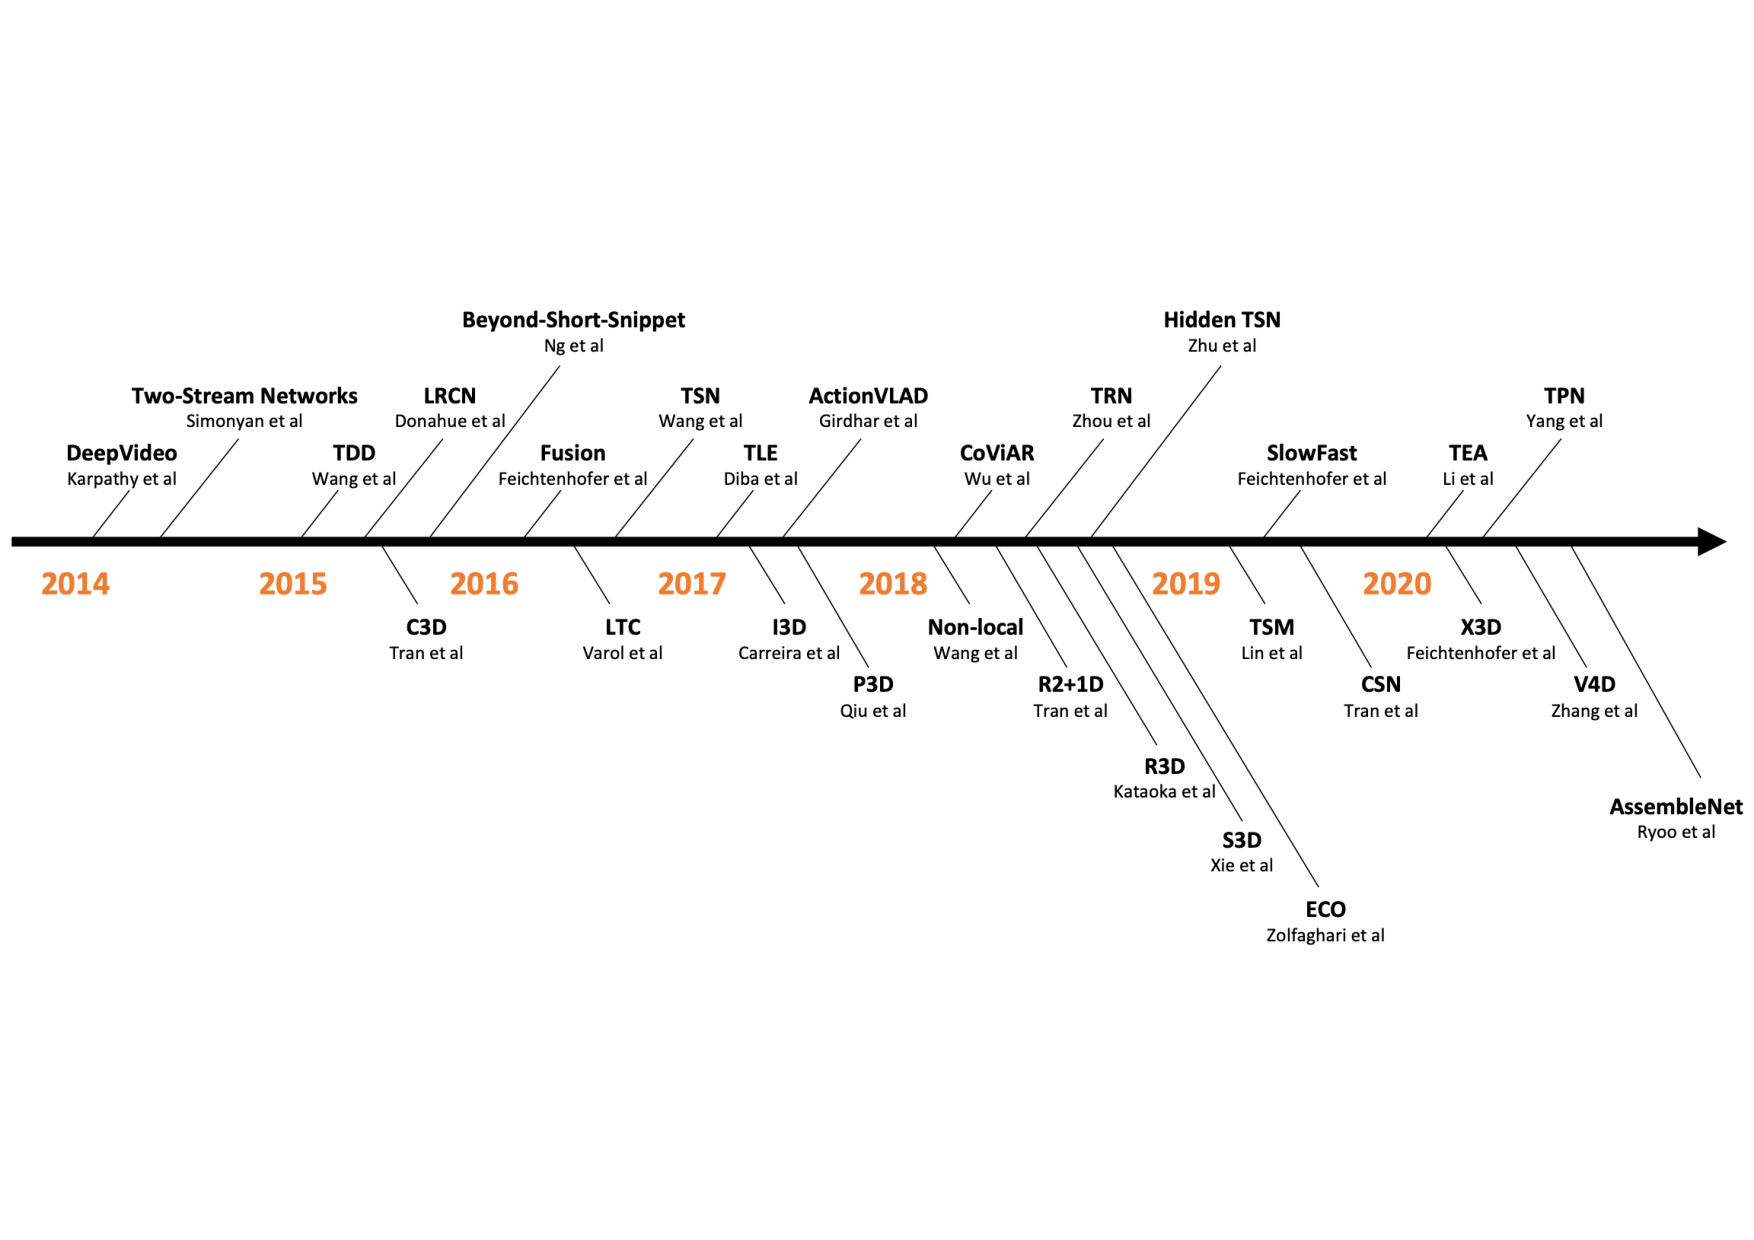
\includegraphics[width=\textwidth]{graphics/summery_ar.pdf}
    \caption{A chronological overview of representative work in video action recognition before 2020 \cite{zhu2020comprehensive}.}
    \label{fig:summery_ar}
\end{figure}

There are several challenges in developing effective video action recognition algorithms. First, some human actions are closely related and exhibit similar movement patterns, making it difficult for algorithms to distinguish between them. The second significant challenge is that the model needs to simultaneously understand both short-term information and long-term temporal information. 

Wang et al. \cite{WangXW0LTG16} proposed the \gls{tsn} to address the challenge of simultaneously understanding short-term and long-term information. The structure of \gls{tsn} is a  common example of \gls{cnn}-based models. Figure \ref{fig:tsn} shows a simplified structure of \gls{tsn}. \gls{tsn} performs video-level action recognition, by taking the entire video as input and segmenting it into several parts, uniformly distributed along the temporal dimension. \gls{tsn} then randomly selects a frame within each segment and sends it to subsequent layers. Finally, the information from the sampled frame is aggregated in the Segmental Consensus module. This segmental structure allows \gls{tsn} to observe content throughout the entire video. Many follow-up studies have handled short-term and long-term content using a similar strategy. Resently, Lin et al. \cite{lin_tsm_2019} introduced the \gls{tsm}. The part of the channels will be shifted along the temporal dimension, thereby facilitating the exchange of information among neighboring frames.

\begin{figure}
    \centering
    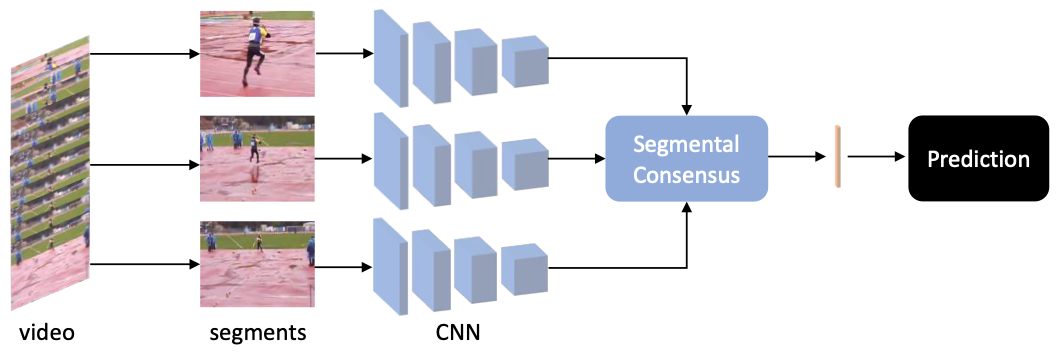
\includegraphics[width=\textwidth]{graphics/tsn.png}
    \caption{The structure of \acrfull{tsn} \cite{zhu2020comprehensive}}
    \label{fig:tsn}
\end{figure}

\section{Egocentric Action Recognition}
\label{ear}
Egocentric video, most captured by wearable cameras, are characterized by frequent and large camera movements, along with complex background scenes.
These features present unique challenges for general video transformer models.
Several high-quality egocentric video datasets have been collected in previous studies, including \cite{damen_epic-kitchens_2021}, \cite{sigurdsson_charades-ego_2018} and \cite{sigurdsson_charades-ego_2018}.
Notably, datasets such as Ego4D \cite{grauman_ego4d_2022} provide additional information like gaze, stereo and audio.
This section will review relevant research in egocentric video action recognition. 
Herzi et al. \cite{herzig_object-region_2022} proposed an object-centric module for integration with video transformers.
Wang et al. \cite{wang_symbiotic_2020} propose Symbiotic Attention with Privileged information for EAR.
Additionally, Huang et al. \cite{huang_ego-vision_2020} collected a new egocentric video dataset and developed a graphical model for joint attention detection.
Despite the progress made, previous research has often not fully addressed the specific challenges inherent in egocentric videos.
To this end, Pan et al. \cite{pan_egovit_2023} proposed a pyramid video transformer structure, showing promising results for egocentric video applications.

Other studies have focused on the role of gaze information in egocentric video.
Huang et al. \cite{huang_predicting_2018} incorporated temporal attention transition into a CNN-based saliency model for gaze estimation.
Tavakoli et al. \cite{tavakoli_digging_2019} explored both bottom-up and top-down attentional cues involved in first-person gaze guidance.
Furthermore, Lai et al. \cite{lai_eye_2022} introduces a transformer-based model that explicitly embeds global context and calculates spatio-temporal global-local correlation for egocentric gaze estimation.
In this thesis, our aim is to develop a transformer for egocentric video, building upon the EgoViT framework and incorporating DCTG with gaze information.

\section{Transformer}
\label{transformer}
Transformer is a new deep learning architecture first introduced in the paper "Attention is All You Need" by Vaswani et al. \cite{vaswani_attention_2023} in 2017. Originally used primarily for \gls{nlp} tasks, the Transformer architecture has demonstrated the ability to handle large amounts of text data effectively. Its breakthrough achievements have made Transformers a fundamental component in \gls{nlp}. The key component of the Transformer is its Attention Mechanism. The attention function is defined as mapping a query and a set of key-value pairs to an output, with the query, keys, values, and output all being vectors \cite{vaswani_attention_2023}. Figure \ref{fig:attention} visualizes the principle of the attention mechanism. The scaled dot-product attention is calculated as follows:
\begin{equation}
\text{Attention}(Q, K, V) = \text{softmax}\left(\frac{QK^T}{\sqrt{d_k}}\right) V
\end{equation}
Where $Q$ is the query, $K$ is keys, $V$ is the values, and $d_k$ is the dimension of the keys.
% \begin{figure}
%     \centering
%     \subfloat[Scaled Dot-Product Attention]{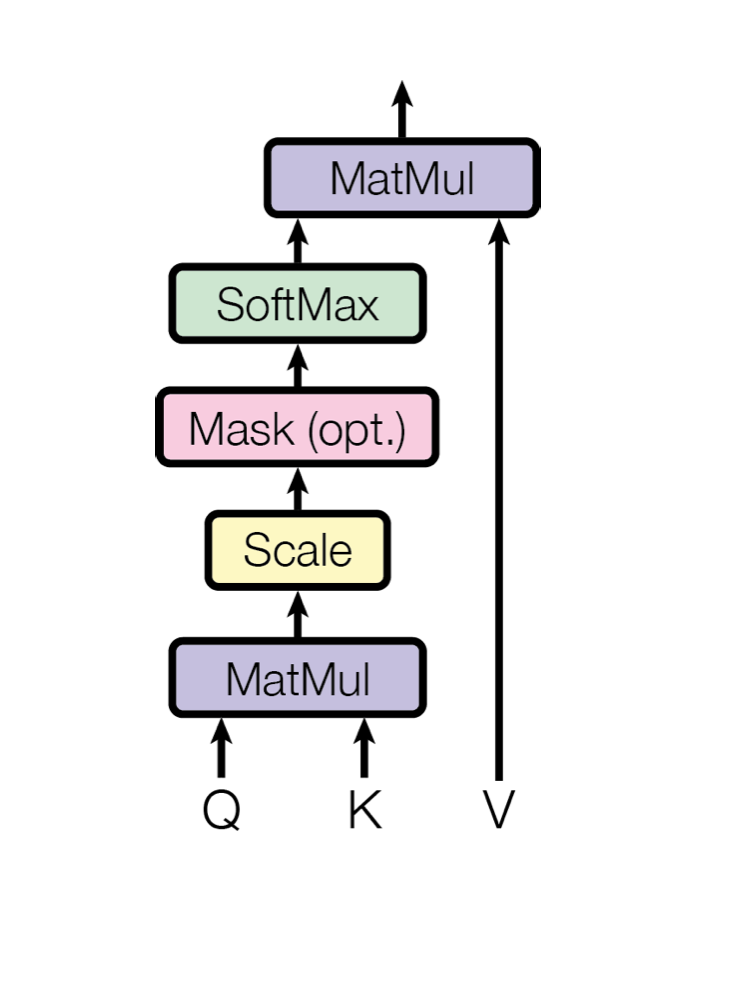
\includegraphics[width=0.4\textwidth]{graphics/attention_mech1.png}\label{fig:attention1}}
%     \hfill
%     \subfloat[Multi-Head Attention]{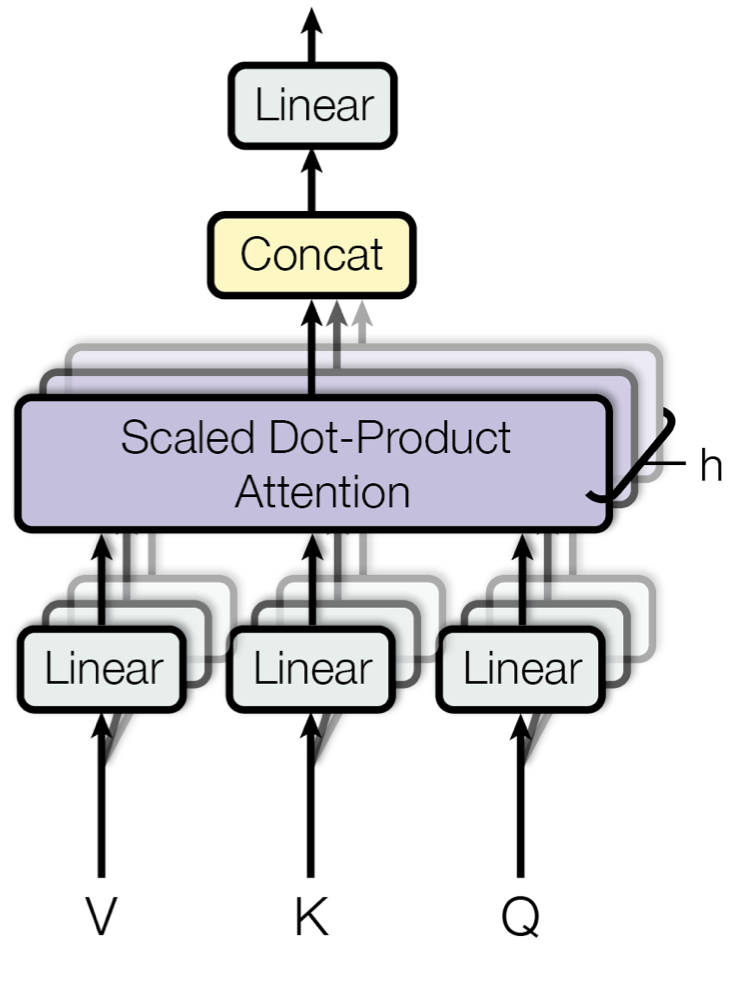
\includegraphics[width=0.4\textwidth]{graphics/attention_mech2.png}\label{fig:attention2}}
%     \caption{The schema of Scaled Dot-Product Attention Figure (a) and Multi-Head Attention Figure (b)}
%     \label{fig:attention}
% \end{figure}
\begin{figure}[htbp]
    \centering
    \subfigure[Scaled Dot-Product Attention]{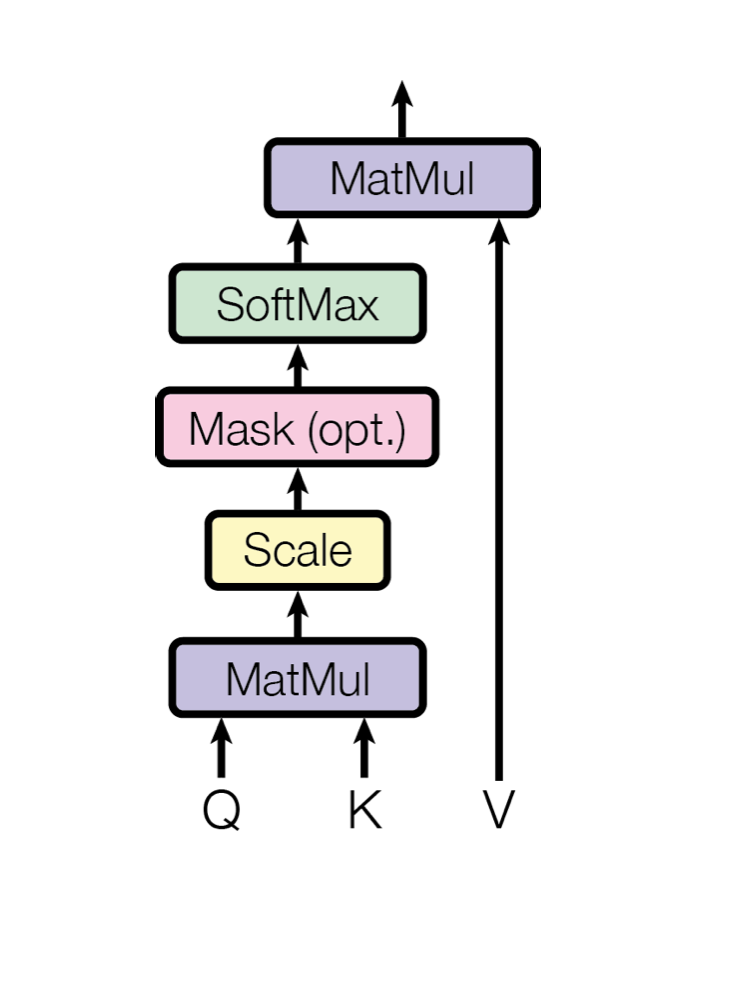
\includegraphics[width=0.4\textwidth]{graphics/attention_mech1.png}\label{fig:attention1}}
    \hfill
    \subfigure[Multi-Head Attention]{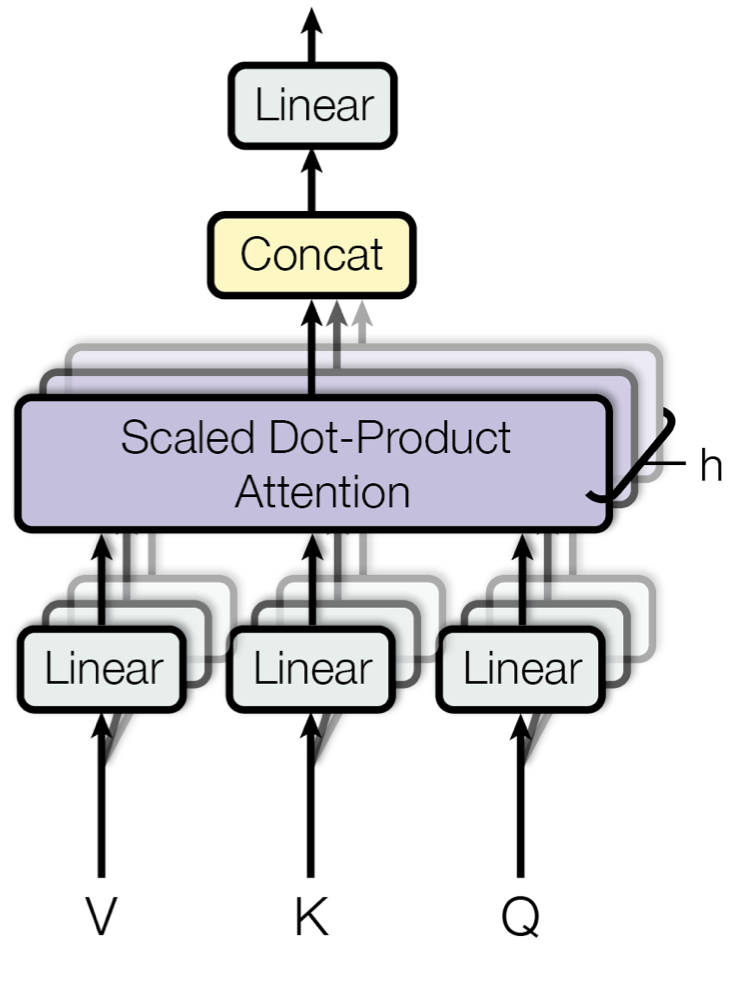
\includegraphics[width=0.4\textwidth]{graphics/attention_mech2.png}\label{fig:attention2}}
    \caption{The schema of Scaled Dot-Product Attention (a) \cite{vaswani_attention_2023} and Multi-Head Attention (b) \cite{vaswani_attention_2023}}
    \label{fig:attention}
\end{figure}
Multiple single attention function with $d_{model}$-dimension keys, values and queries are applied, and their outputs are concatenated to form the Multi-Head Attention. Hence, the Multi-Head can be described as follows:
\begin{equation}
\begin{aligned}
\text{MultiHead}(Q, K, V) &= \text{Concat}(\text{head}_1, \ldots, \text{head}_h) W^O \\
\text{where } \text{head}_i &= \text{Attention}(Q W_i^Q, K W_i^K, V W_i^V)
\end{aligned}
\end{equation}
Where $W_i^Q \in \mathbb{R}^{d_{\text{model}} \times d_k}$, $W_i^K \in \mathbb{R}^{d_{\text{model}} \times d_k}$, $W_i^V \in \mathbb{R}^{d_{\text{model}} \times d_v}$, and $W^O \in \mathbb{R}^{h d_v \times d_{\text{model}}}$.

The transformer can be divided into two parts: the Encoder and the Decoder. Each part consists of stacked identical layers, a multi-head self-attention mechanism and a feed-forward neural network. The decoder additionally includes a masked multi-head self-attention mechanism, which ensures that predictions for a given position depend only on the known outputs at previous positions \cite{vaswani_attention_2023}. The structure of the transformer is shown in Figure \ref{fig:transformer}. The self-attention mechanism has demonstrated its ability to learn the long-range dependencies. Building on the success of transformers in \gls{nlp}, several studies have explored combining \gls{cnn}-based architectures with self-attention \cite{wang_Non-local_2017}, \cite{carion_End-to-End_2020}. However, a major drawback of these models is that The global properties of self-attention may not be fully utilized during the integration of two mechanism. While they are effective at capturing local features and extracting spatial information in small areas through convolution kernels, they are less effective at capturing global information.
% Dosovitskiy et al. \cite{dosovitskiy_image_2021} proposed the \gls{vit} for image recognition. \gls{vit}, with minimal modifications from transformer, achieves excellent results compared to state-of-the-art convolutional networks. Their work has demonstrated that a pure transformer architecture is a promising solution for image recognition.
\begin{figure}
    \centering
    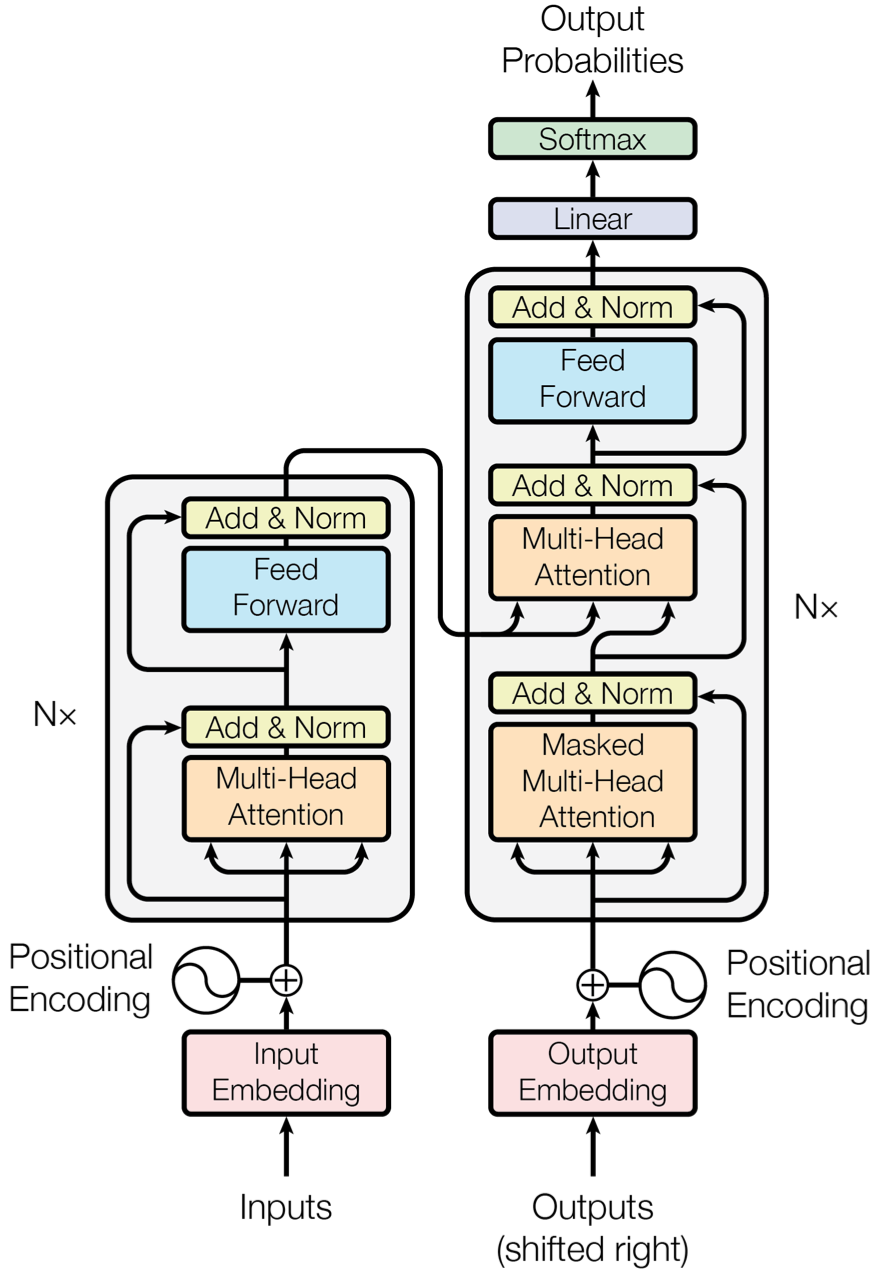
\includegraphics[width=0.6\textwidth]{graphics/structure_transformer.png}
    \caption{The structure of transformer \cite{vaswani_attention_2023}.}
    \label{fig:transformer}
\end{figure}

\section{Transformers in Video Recognition}
\label{sec:Transformers in Video Recognition}
Dosovitskiy et al. \cite{dosovitskiy_image_2021} proposed the \gls{vit} for image recognition. \gls{vit}, which globally models spatial relationships on non-overlapping image patches with minimal modifications from standard transformer \cite{vaswani_attention_2023}, achieves excellent results compared to state-of-the-art convolutional networks. Their work has demonstrated that a pure transformer architecture is a promising solution for image recognition. Following the success of \gls{vit} in image classification, multiple works have tried to explore transformer-based architectures for video recognition. Extending these advancements to video data, which adds only a spatial domain compared to image data, researchers have adapted these transformative techniques on the transformer-based model. Recently, Arnab et al. \cite{arnab_vivit_2021} presented a pure-transformer based model for video classification. The \gls{vivit} calculates a sequence of spatiotemporal tokens from input video, then processes them with self-attention. By employing several methods to factorize the model along spatial and temporal dimensions, \gls{vivit} is able to handle long-distance dependencies and complex spatiotemporal interactions effectively.

As a result, Video Transformers \cite{bertasius_is_2021}, \cite{liu_video_2021}, \cite{herzig_object-region_2022}, \cite{neimark_video_2021}, which inherit the advantages of image understanding from their predecessors, have shown remarkable success in video recognition benchmarks \cite{russakovsky_imagenet_2015}, \cite{kay_kinetics_2017}. Despite the excellent success video transformer have achieved, some video transformers like \cite{arnab_vivit_2021}, \cite{bertasius_is_2021}, \cite{neimark_video_2021} suffer from high computation costs, primarily due to extending the image spatial domain into a global spatiotemporal domain. Another disadvantage is that the performance of these video transformers heavily relies on pretrained 2D spatial models on super large dataset JFT-300M \cite{Sun_Rev_2017}. The third challenge for video transformers is the efficiency of processing long-range dependencies.  In practice, when processing long videos, important temporal information may be diluted or overshadowed by a large number of attention weights.

To address this issue, Liu et al. \cite{liu_video_2021} attempted to overcome this limitation by broadening the focus of local attention computation.
Instead of solely concentrating on the spatial domain, their approach encompasses both spatial and temporal domains. Pan et al. \cite{pan_egovit_2023} emphasize the importance of both local and global temporal attention, especially for egocentric videos, which typically contain large and frequent movements. To effectively address these problems, they proposed a pyramid structure that successfully integrates both local and global temporal attentions. This structure provides an inductive bias on grouping both local temporal attentions and the global temporal attentions \cite{pan_egovit_2023}.
In section \ref{sec:Video Swin Transformer}, the Video Swin Transformer will be discussed in detail, as it serves as the backbone of the proposed model in this thesis.

\section{Object Detection-Oriented Action Recognition}
\label{sec:Object detection-orientated video action recognition}
A number of studies \cite{ferrari_compositional_2018}, \cite{wang_symbiotic_2020}, \cite{baradel_object_2018}, \cite{xu_learning_2019} have demonstrated that models incorporating object detection and interaction features, particularly those focusing on object-human interactions, achieve considerable success in the field of video understanding.
More recently, research has focus on video action recognition with egocentric video.
Shvetsova et al. \cite{shvetsova_everything_2022} proposed a modality-agnostic transformer that integrates information from various sources into a single multi-modal representation.
Herzig et al. \cite{herzig_object-region_2022} introduced the Object-Dynamics Module, which achieved state-of-the-art performance in video action recognition.
Drawing inspiration from Herzig et al. \cite{herzig_object-region_2022}, Pan et al. \cite{pan_egovit_2023} designed the first method to incorporate object-human interaction features into a transformer.
This is achieved through a dynamic class token, embedding these features directly into the class token \cite{pan_egovit_2023}.
Their method addresses two key issues: firstly, how to incorporate object-subject interaction features, and secondly, how to embed locality inductive bias within the self-attention module.

\section{Video Swin Transformer}
\label{sec:Video Swin Transformer}
The Video Swin Transformer builds on the Swin Transformer, extending the local attention computation from solely the spatial domain to the spatiotemporal domain. The overall architecture is shown in Figure \ref{fig:swin-transformer}. Video Swin Transformer consist of four stages, each containing a patch merging layer and multiple Video Swin Transformer Block. The transformer block will be repeated $N$ times according to the model configuration. It does not down-sample along the temporal dimension, but performs $2\times$ spatial down-sampling in the patch merging layer of each stage. The input videos will be divided into several 3D patches. The patches are then processed through the stages in series. The output of the last stage is defined as the normal token, which is used for classification in subsequent head layers.
% \clearpage
\begin{figure}[htbp]
    \centering
    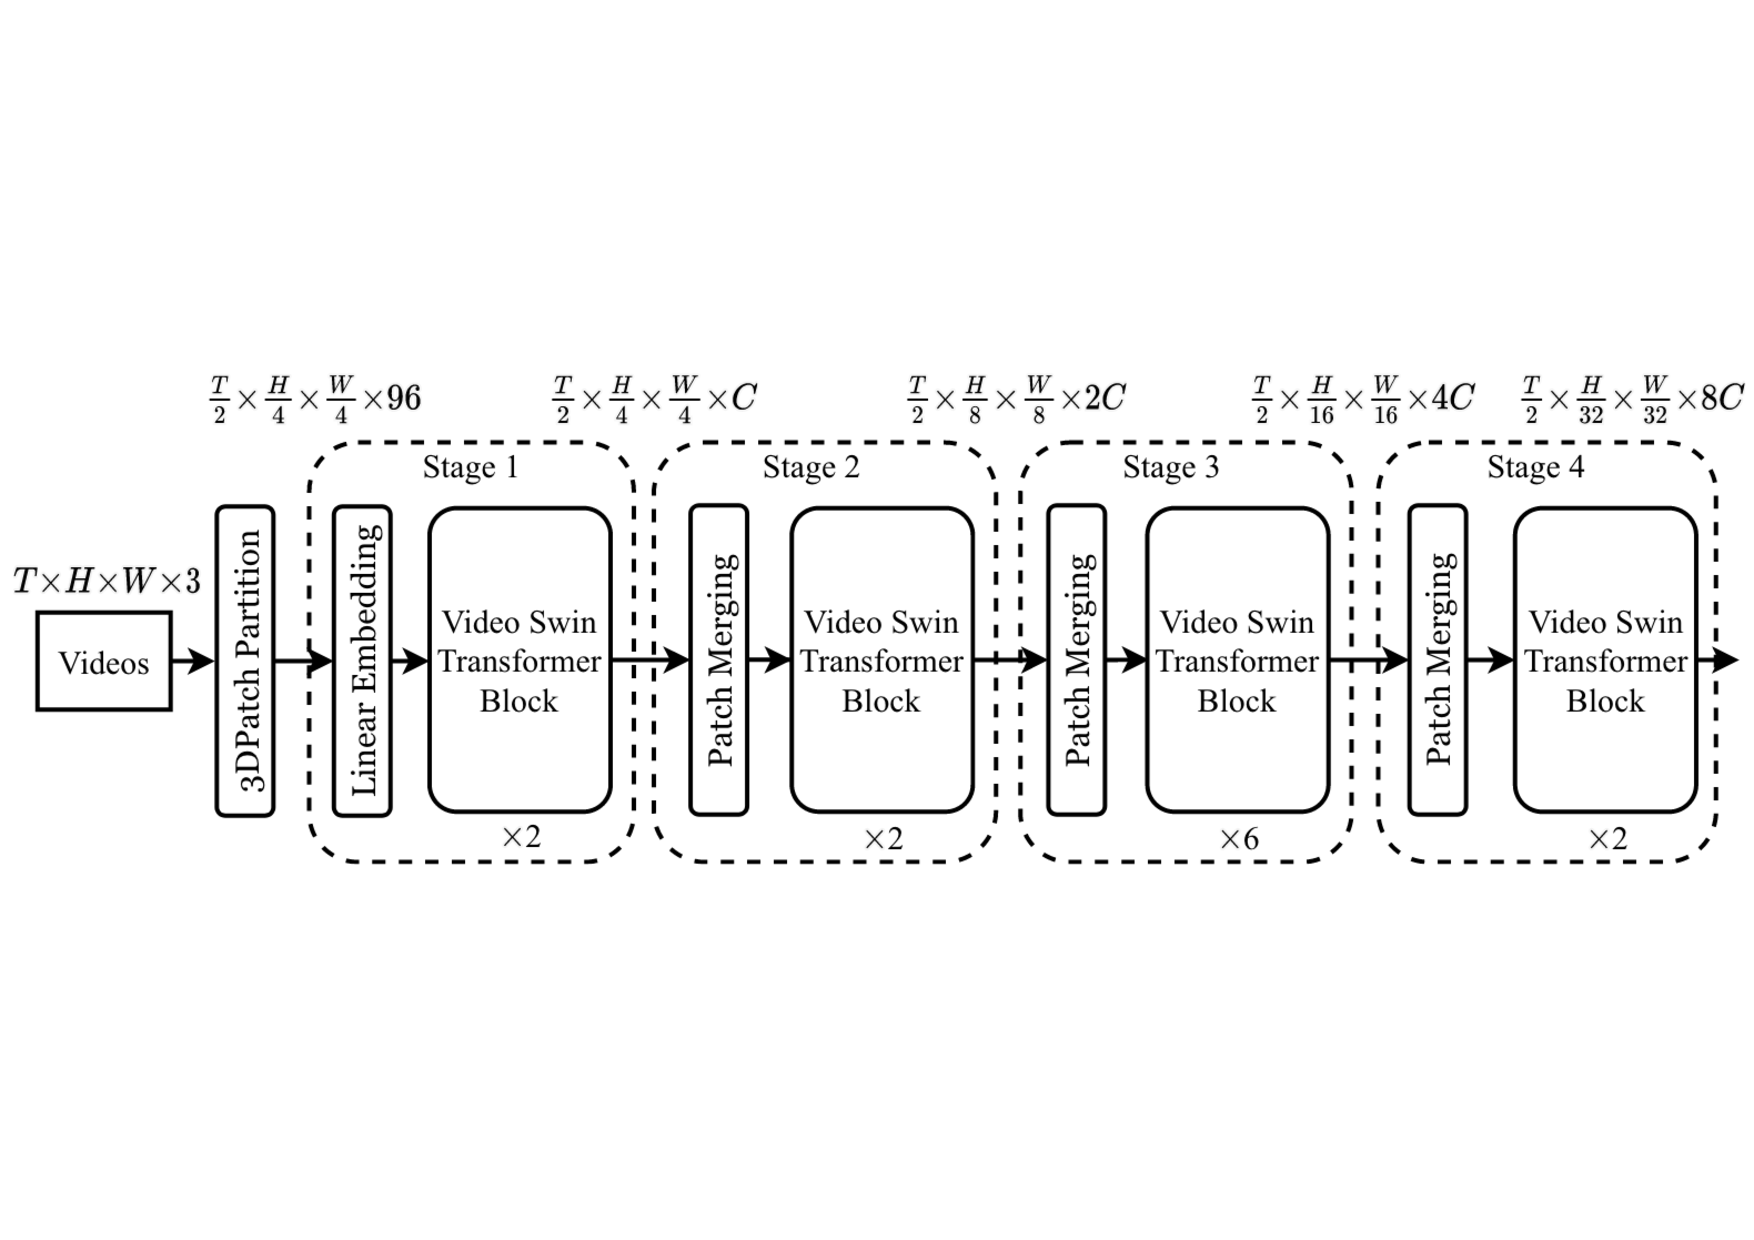
\includegraphics[width=\textwidth]{graphics/Swin_overview.pdf}
    \caption{The architecture of Video Swin Transformer (Swin-T version) \cite{liu_video_2021}.}
    \label{fig:swin-transformer}
\end{figure}

The Video Swin Transformer Block inherit the structure of standard transformer, only replacing the \gls{msa} with the 3D shifted window based multi-head self-attention module. As shown in Figure \ref{fig:swin-block}, a Video Swin Transformer Block consists of a 3D shifted windows based \gls{msa} module, a \gls{ffn}, and two \gls{ln} layers before the 3D SW-\gls{msa} and \gls{ffn}. Through the 3D shifted windows based \gls{msa}, the Video Swin Transformer introduces a locality inductive bias to the self-attention module. The shifted windows allow the non-overlapping 3D windows to exchange information with each other. Figure \ref{fig:swin-msa} illustrate the mechanism of the 3D shifted windows based \gls{msa} module. 
\vspace{5mm}

\begin{figure}[htbp]
    \centering
    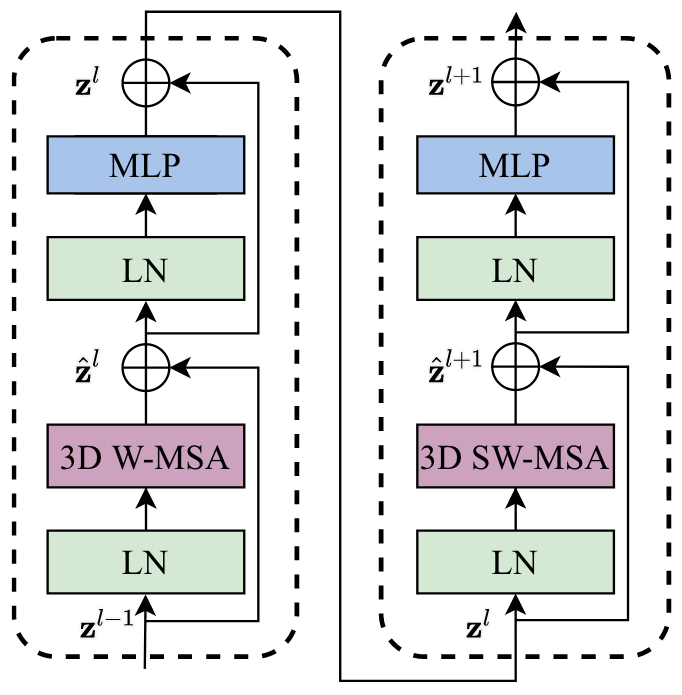
\includegraphics[width=0.5\textwidth]{graphics/swin_t_block.png}
    \caption{The structure of Video Swin Transformer Block \cite{liu_video_2021}.}
    \label{fig:swin-block}
\end{figure}
\clearpage
\vspace{5mm}
\begin{figure}[htbp]
    \centering
    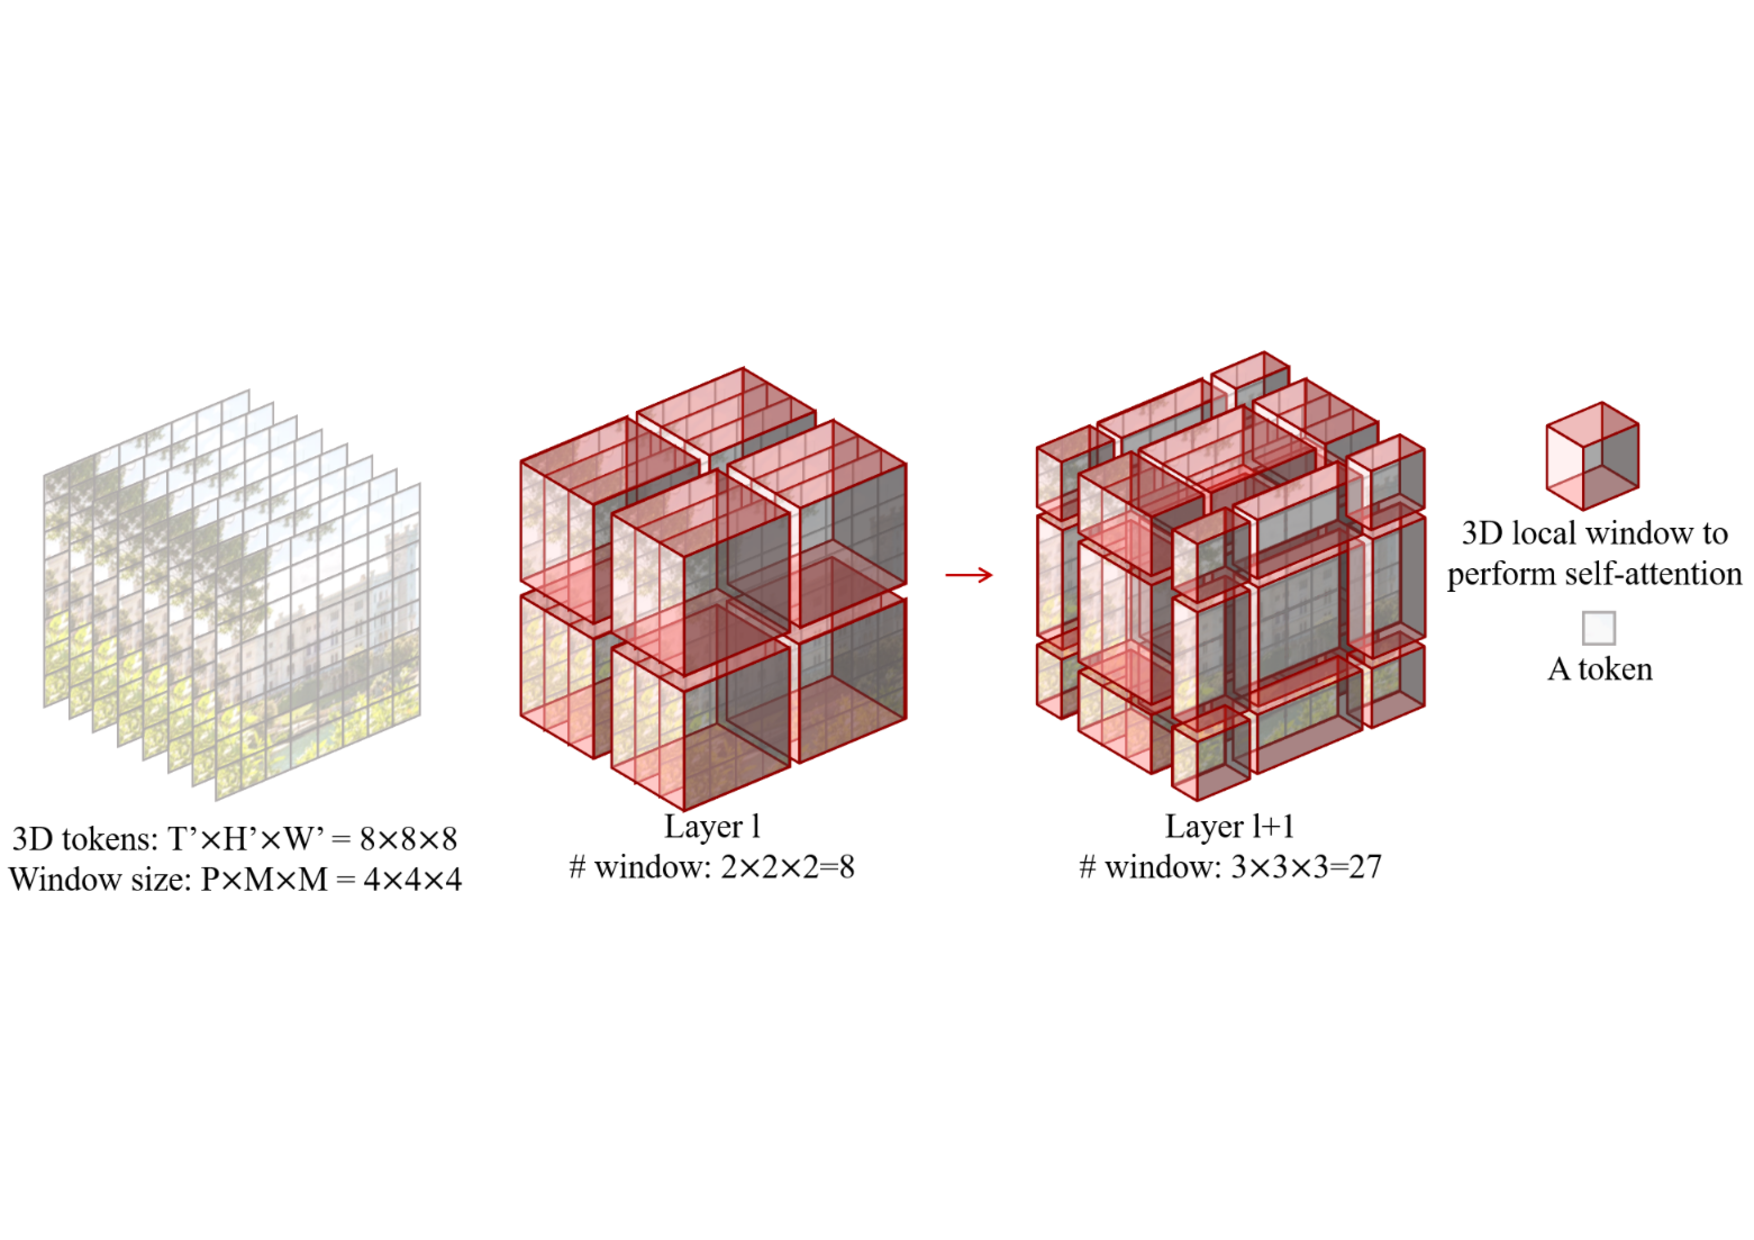
\includegraphics[width=\textwidth]{graphics/shift_window.pdf}
    \caption{The mechanism of 3D shifted windows \cite{liu_video_2021}.}
    \label{fig:swin-msa}
\end{figure}

\section{EgoViT}
\label{sec:EgoViT}
In this section, the structure and key components of EgoViT will be explained in detail. Since the proposed model in this thesis is strictly based on EgoViT, it is important to thoroughly understand the structure of EgoViT.

EgoViT features a hierarchical pyramid structure that effectively provides an inductive bias for grouping both local and global temporal attentions. This design enables it to successfully process the rapid motions typically found in egocentric videos. The overall architecture of EgoViT is shown in Figure \ref{fig:egovit}. EgoViT consists of three main parts: the Short-term Stage, Intermediate Connection and Long-term Stage.
\begin{figure}[b]
    \centering
    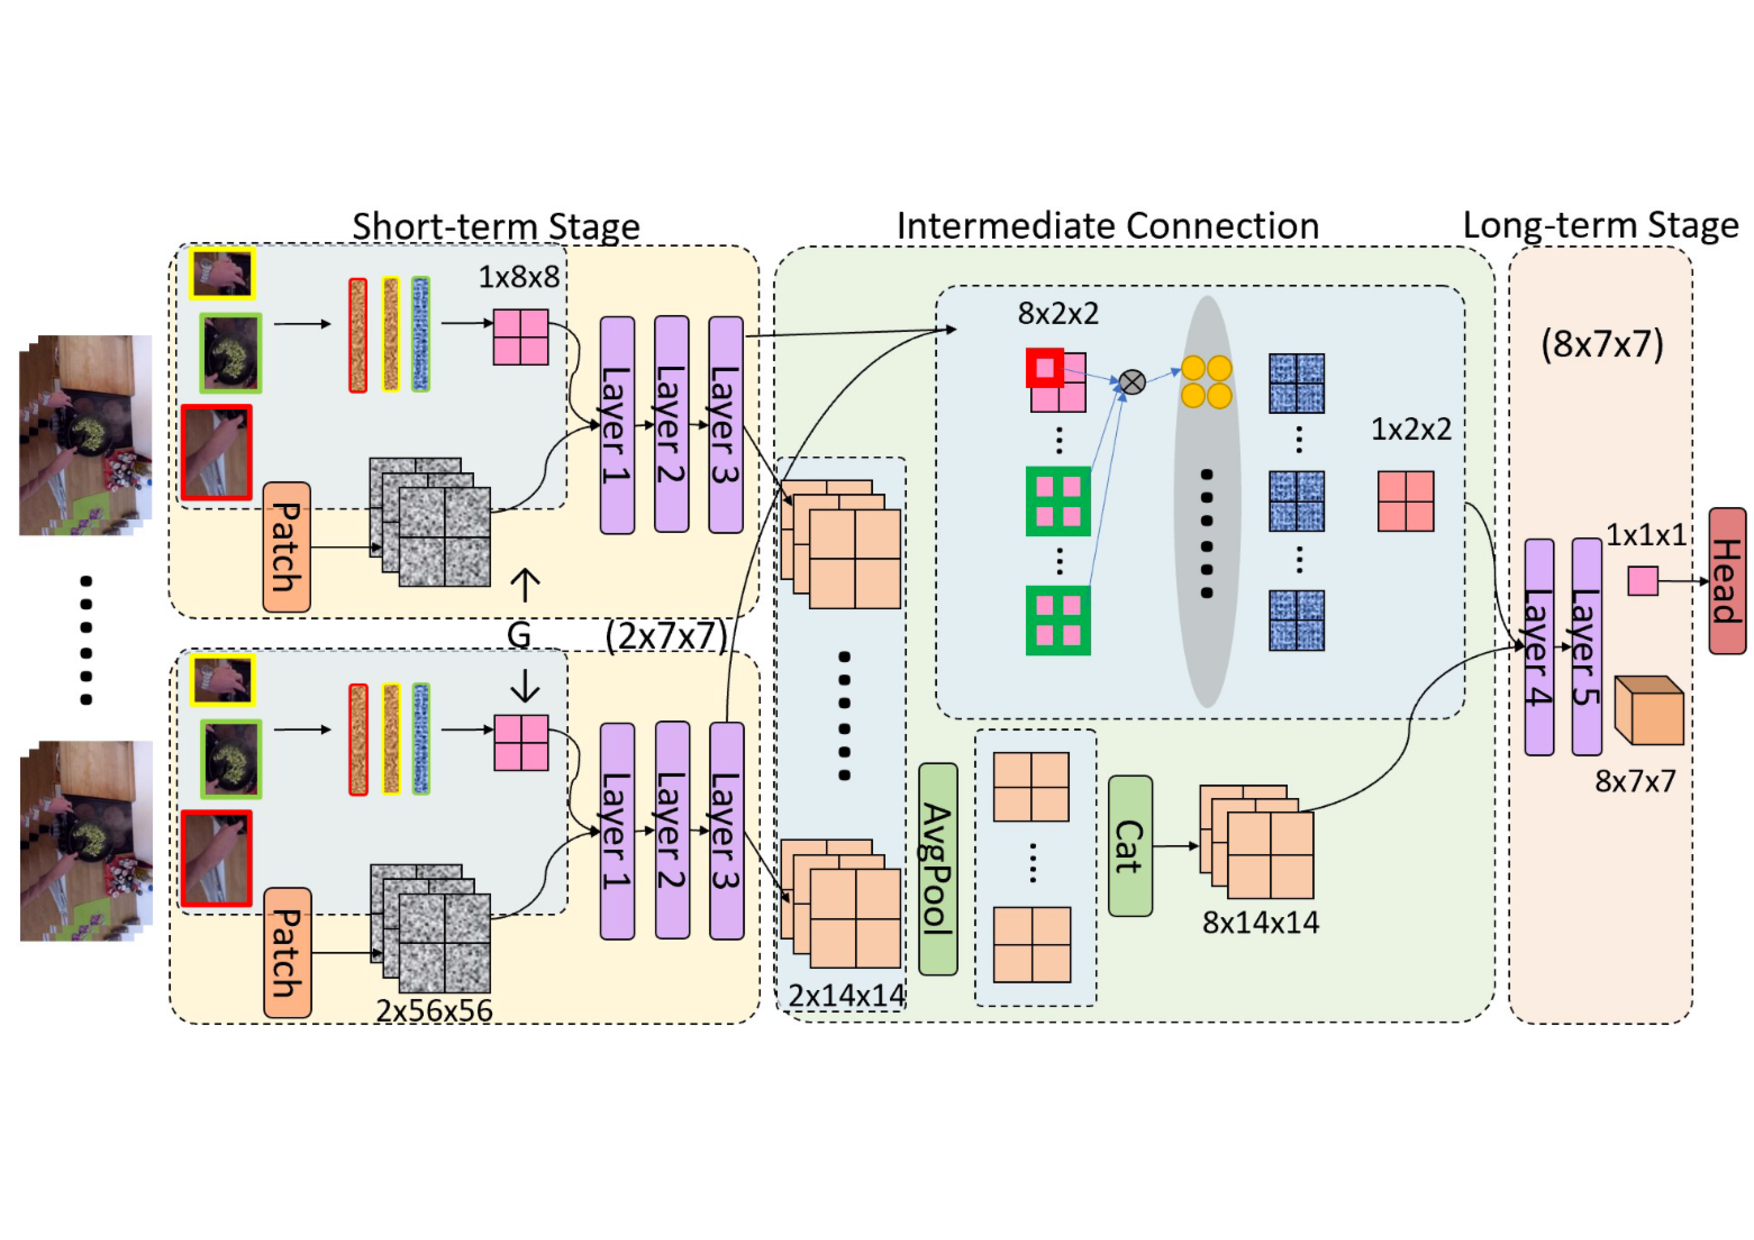
\includegraphics[width=\textwidth]{graphics/egovit.pdf}
    \caption{The architecture of EgoViT with Dynamic Class Token Generator\cite{pan_egovit_2023}.}
    \label{fig:egovit}
\end{figure}

The Short-term Stage is designed to capture the local temporal information. It is divided into $G$ groups, and each group integrates a \gls{dctg} module. The \gls{dctg} contains a pretrained \gls{hod} module, which detects the hands and objects interacting within the frames. The detected hands and objects are transformed as a combined hand-object features. These combined hand-object features are then processed in subsequent layers to generate the \gls{dct}. The \gls{dct}s are concatenated with the embedded frames for the following transformer layers. After processing in these layers, the $G$ \gls{dct}s provide a summary of the semantic meaning of each short video phase. The processed \gls{dct}s from each group are then merged in the Intermediate Connection. During this merging process, a larger weight is assigned to the \gls{dct}s that represent crucial short-term actions.
The merging process can be expressed in Eq. \ref{eq:x_cls_s}
\begin{align}
    \alpha_{g,s,g'} &= \frac{1}{\|\mathbf{x}^{cls}_{g,s}\|} \sum_{s'} \frac{\mathbf{x}^{cls}_{g,s} \cdot \mathbf{x}^{cls}_{g',s'}}{\|\mathbf{x}^{cls}_{g',s'}\|}, \notag \\
    \alpha_{g,s} &= \sum_{g' \neq g} \alpha_{g,s,g'}, \notag \\
    \mathbf{x}^{cls}_{s} &= \sum_{g} \mathbf{x}^{cls}_{g,s} \frac{\exp(\alpha_{g,s})}{\sum_{\bar{g}} \exp(\alpha_{\bar{g},s})} \label{eq:x_cls_s}
    \end{align}

Where $g$ and $g'$ are group indices, $s$ and $s'$ are spatial indices, $\alpha_{g,s,g'}$ is the score of one group, $\alpha_{g,s}$ is the total score of all groups, and $x^{cls}_s$ is the weighted class token.

The weighted class token contains information about the actions from the $G$ phases. The layers in the long-term stage aim to perceive actions over long durations and under significant scene changes by exploring the inter-relationships of the short-term actions \cite{pan_egovit_2023}. The structure of the EgoViT addresses the challenges of egocentric video action recognition, such as large-scale scene changes between distant frames and the varying contributions of nearby frames.

% \subsection{Egocentric Video Action Recognition}
% \label{Egocentric Video Action Recognition}
% Egocentric video, most captured by wearable cameras, are characterized by frequent and large camera movements, along with complex background scenes.
% These features present unique challenges for general video transformer models.
% Several high-quality egocentric video datasets have been collected in previous studies, including \cite{damen_epic-kitchens_2021}, \cite{sigurdsson_charades-ego_2018} and \cite{sigurdsson_charades-ego_2018}.
% Notably, datasets such as Ego4D \cite{grauman_ego4d_2022} provide additional information like gaze, stereo and audio.
% This section will review relevant research in egocentric video action recognition. 
% Herzi et al. \cite{herzig_object-region_2022} proposed an object-centric module for integration with video transformers.
% Wang et al. \cite{wang_symbiotic_2020} propose Symbiotic Attention with Privileged information for EAR.
% Additionally, Huang et al. \cite{huang_ego-vision_2020} collected a new egocentric video dataset and developed a graphical model for joint attention detection.
% Despite the progress made, previous research has often not fully addressed the specific challenges inherent in egocentric videos.
% To this end, Pan et al. \cite{pan_egovit_2023} proposed a pyramid video transformer structure, showing promising results for egocentric video applications.

% Other studies have focused on the role of gaze information in egocentric video.
% Huang et al. \cite{huang_predicting_2018} incorporated temporal attention transition into a CNN-based saliency model for gaze estimation.
% Tavakoli et al. \cite{tavakoli_digging_2019} explored both bottom-up and top-down attentional cues involved in first-person gaze guidance.
% Furthermore, Lai et al. \cite{lai_eye_2022} introduces a transformer-based model that explicitly embeds global context and calculates spatio-temporal global-local correlation for egocentric gaze estimation.
% In this thesis, our aim is to develop a transformer for egocentric video, building upon the EgoViT framework and incorporating DCTG with gaze information.

% \subsection{Transformers in Video Recognition}
% \label{Transformers in Video Recognition}
% Recently, Vaswani et al. \cite{vaswani_attention_2023} introduced self-attention layers, which have significantly enhanced the field of natural language processing by replacing traditional CNN and RNN layers, achieving state-of-the-art results.
% In a separate study, Dosovitskiy et al. \cite{dosovitskiy_image_2021} demonstrate that a Vision Transformer (ViT) is particularly effective for image classification tasks, especially when applied to a super large dataset such as 300M JFT \cite{Sun_Rev_2017}.
% Extending these advancements to video data, which adds only a spatial domain compared to image data, researchers have adapted these transformative techniques on the transformer-based model.
% As a result, Video Transformers \cite{arnab_vivit_2021}, \cite{bertasius_is_2021}, \cite{liu_video_2021}, \cite{herzig_object-region_2022}, \cite{neimark_video_2021}, which inherit the advantages of image understanding from their predecessors, have shown remarkable success in video recognition benchmarks \cite{russakovsky_imagenet_2015}, \cite{kay_kinetics_2017}.
% Some video transformers \cite{arnab_vivit_2021}, \cite{bertasius_is_2021}, \cite{neimark_video_2021} suffer from high computation costs, primarily due to extending the image spatial domain into a global spatio-temporal domain.
% Another disadvantage is that the performance of these video transformers heavily relies on pretrained 2D spatial models on super large dataset JFT-300M \cite{Sun_Rev_2017}.
% To address this issue, Liu et al. \cite{liu_video_2021} attempted to overcome this limitation by broadening the focus of local attention computation.
% Instead of solely concentrating on the spatial domain, their approach encompasses both spatial and temporal domains.
% Pan et al. \cite{pan_egovit_2023} emphasize the importance of both local and global temporal attention, especially for egocentric videos, which typically contain large and frequent movements.
% To effectively address these problems, they proposed a pyramid structure that successfully integrates both local and global temporal attentions.
% This structure provides an inductive bias on grouping both local temporal attentions and the global temporal attentions \cite{pan_egovit_2023}.

% \subsection{Object detection-orientated video action recognition} 
% \label{Object detection-orientated video action recognition}
% A number of studies \cite{ferrari_compositional_2018}, \cite{wang_symbiotic_2020}, \cite{baradel_object_2018}, \cite{xu_learning_2019} have demonstrated that models incorporating object detection and interaction features, particularly those focusing on object-human interactions, achieve considerable success in the field of video understanding.
% More recently, research has focus on video action recognition with egocentric video.
% Shvetsova et al. \cite{shvetsova_everything_2022} proposed a modality-agnostic transformer that integrates information from various sources into a single multi-modal representation.
% Herzig et al. \cite{herzig_object-region_2022} introduced the Object-Dynamics Module, which achieved state-of-the-art performance in video action recognition.
% Drawing inspiration from Herzig et al. \cite{herzig_object-region_2022},Pan et al. \cite{pan_egovit_2023} designed the first method to incorporate object-human interaction features into a transformer.
% This is achieved through a dynamic class token, embedding these features directly into the class token \cite{pan_egovit_2023}.
% Their method addresses two key issues: firstly, how to incorporate object-subject interaction features, and secondly, how to embed locality inductive bias within the self-attention module.


\chapter{Methodology}
\label{chap:methodology}
In this chapter, the proposed model based on the EgoViT architecture is presented. In this model, the original \gls{dctg} module is extended with the ability to integrate gaze information. Section \ref{sec:Overall Architecture} presents the overall architecture of the proposed model. The extraction of gaze-hand-object features is explained in detail in Section \ref{sec:Gaze-Enhanced DCTG Module}. Modifications made to the Video Swin Transformer \cite{liu_video_2021} to integrate it with the architecture of EgoViT \cite{pan_egovit_2023} are detailed in Section \ref{sec:Integration of Video Swin Transformer}. The dynamic merging algorithms are explained in the last section \ref{sec:Dynamic Merging Module}.

\section{Overall Architecture}
\label{sec:Overall Architecture}
In this thesis work, a Gaze-Enhanced EgoViT model is proposed. The overall architecture is shown in Figure \ref{fig:overall_architecture} and is strictly inherited from the original EgoViT architecture. The model can be divided into three parts: the Short-term Stage, Intermediate Connection, and Long-term Stage. The key components of the model are the Gaze-Enhanced \gls{dctg} module, the modified Video Swin Transformer, and the Dynamic Merging module. In the following sections, the \gls{dctg} in EgoViT will be referred to as the "original \gls{dctg}", while the \gls{dctg} in the proposed model will be referred to as the "gaze-enhanced \gls{dctg}".
\begin{figure}
    \centering
    \rotatebox{90}{%
        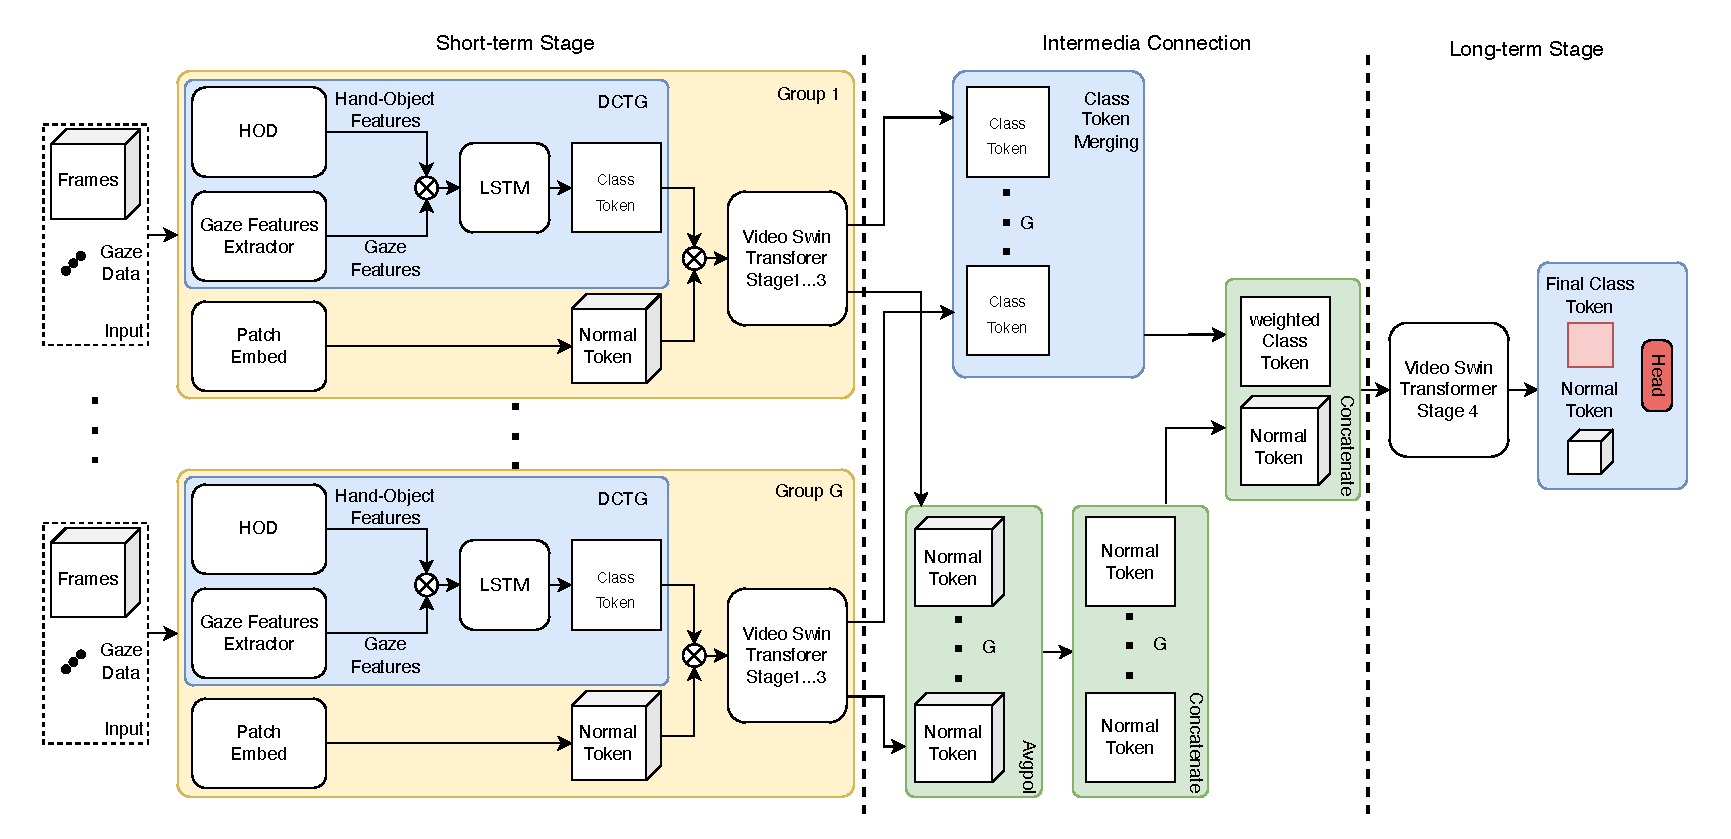
\includegraphics[width=\paperwidth]{graphics/structure.pdf}
    }
    \caption{Overall architecture of the Gaze-Enhanced EgoViT.}
    \label{fig:overall_architecture}
\end{figure}

A Video Transformer commonly converts the input video frames into a sequence of feature vectors. Thus, the input frames can be denoted as the vector $I \in \mathbb{R}^{T_{sampled} \times H\times W\times C}$, where $T_{sampled}$ is the number of frames sampled from the video, $H$ and $W$ are the height and width of the frame, and $C$ is the number of channels. The proposed model includes an additional input of gaze points vector $J \in \mathbb{R}^{T_{sampled} \times 2}$ representing the coordinates $(x, y)$ of the gaze points in the $T_{sampled}$ frames. 

The $T_{sampled}$ frames and their associated $T_{sampled}$ gaze points data are first split into $G$ groups, uniformly distributed along the temporal dimension. The short-term phase of a video clips is denoted as $I_{g} \in \mathbb{R}^{T \times H \times W \times C}$ and the vector of gaze points is denoted as $J_{g} \in \mathbb{R}^{T \times 2}$, where $D = \frac{D_{sampled}}{G}$. The vectors $I_{g}$ and $J_{g}$ are then fed into the Gaze-Enhanced \gls{dctg} module to extract the gaze-hand-object features. The function of Gaze-Enhanced \gls{dctg} will be discussed in detail in section \ref{sec:Gaze-Enhanced DCTG Module}. In parallel, the $I_{g}$ is fed into the PatchEmbedding module in the Video Swin Transformer to extract the features of the video frames. 

The Vector $I_{g}$ is segmented into non-overlapping patches, of size $\mathbb{R}^{P_T \times P_H \times P_W \times C}$. These patches are projected in a flatte layer into sequence data of $\mathbb{R}^{N_P \times (P_T \times P_H \times P_W \times C)}$, where $N_P = T_P \times H_P \times W_P = \frac{T}{P_T} \times \frac{H}{P_H} \times \frac{W}{P_W}$. A liner layer uses a matrix of size $\mathbb{R}^{(P_T \times P_H \times P_W \times C) \times D}$ to project the sequence data into a lower dimension $D$. The embedded vector is denoted as $X_P \in \mathbb{R}^{N_P \times D}$. The output of the Gaze-Enhanced \gls{dctg} module is treated as the class token $x_{cls}$ with the shape $\mathbb{R}^{1 \times D}$, and is concatenated with the sequence data $X_P$ to form the input of the Video Swin Transformer. The Combination of $x_{cls}$ and $X_P$ is performed along the temporal dimension, positioning the class token as the first vector in this dimension. The sequence data $X_P$ is defined as normal token in this model. Therefore, the input to the transformer is defined as:
\begin{equation}
    x= [x_{cls}, X_P] \in \mathbb{R}^{(N_P + 1) \times D}
    \label{eq:input_transformer}
\end{equation}
The class token is designed to leverage the information exchange capabilities of the 3D Shifted Window Self-Attention mechanism in Video Swin Transformer, which facilitates the sharing of information between the class token and the normal token.

The Video Swin Transformer is modified to build the short-term, intermediate and long-term architecture. It is divided in two parts: the PatchEmbedding layers and stage 1 to stage 3 are in the short-term stage, which is responsible for extracting local temporal information. The stage 4 is in the long-term stage, which is responsible for extracting global temporal information. Between the two parts of the Video Swin Transformer, the Dynamic Merging module is used to merge the output of the short-term stage. It calculates the score $\alpha$ of short-term class token for each group. Then, all scores are summed and normalized to obtain the total score $\alpha_{total}$. A weighted class token is then calculated from $\alpha_{total}$ and the class tokens $x^{cls}_g$ of each group. In this module, the weights are assigned, and the class tokens are aggregated based on the short-term actions. The Dynamic Merging module is discussed in detail in section \ref{sec:Dynamic Merging Module}.

The input of long-term stage is the concatenation of the weighted class token $x^{cls}_{st}$ and the normal token $X^{P}_{st}$, where the subscript "st" for short-term. Therefore, the input of the long-term stage is defined as:
\begin{equation}
    x_{lt} = [x^{cls}_{st}, X^{P}_{st}] \in \mathbb{R}^{(N_P + 1) \times D_{st3}}
    \label{eq:input_long_term}
\end{equation}
Where $D_{st}$ is the dimension of the output of the stage3 in Video Swin Transformer and the subscript "lt" denotes for long-term. 

The $x_{lt}$ is fed into the stage 4 of Video Swin Transformer to extract the global temporal information. The final score of the action prediction is calculated from the Head, which computes the score of each action class. The action class with the highest score is selected as the final prediction.
% \begin{landscape}
%     \centering
%     \begin{figure}
%         \centering
%         % 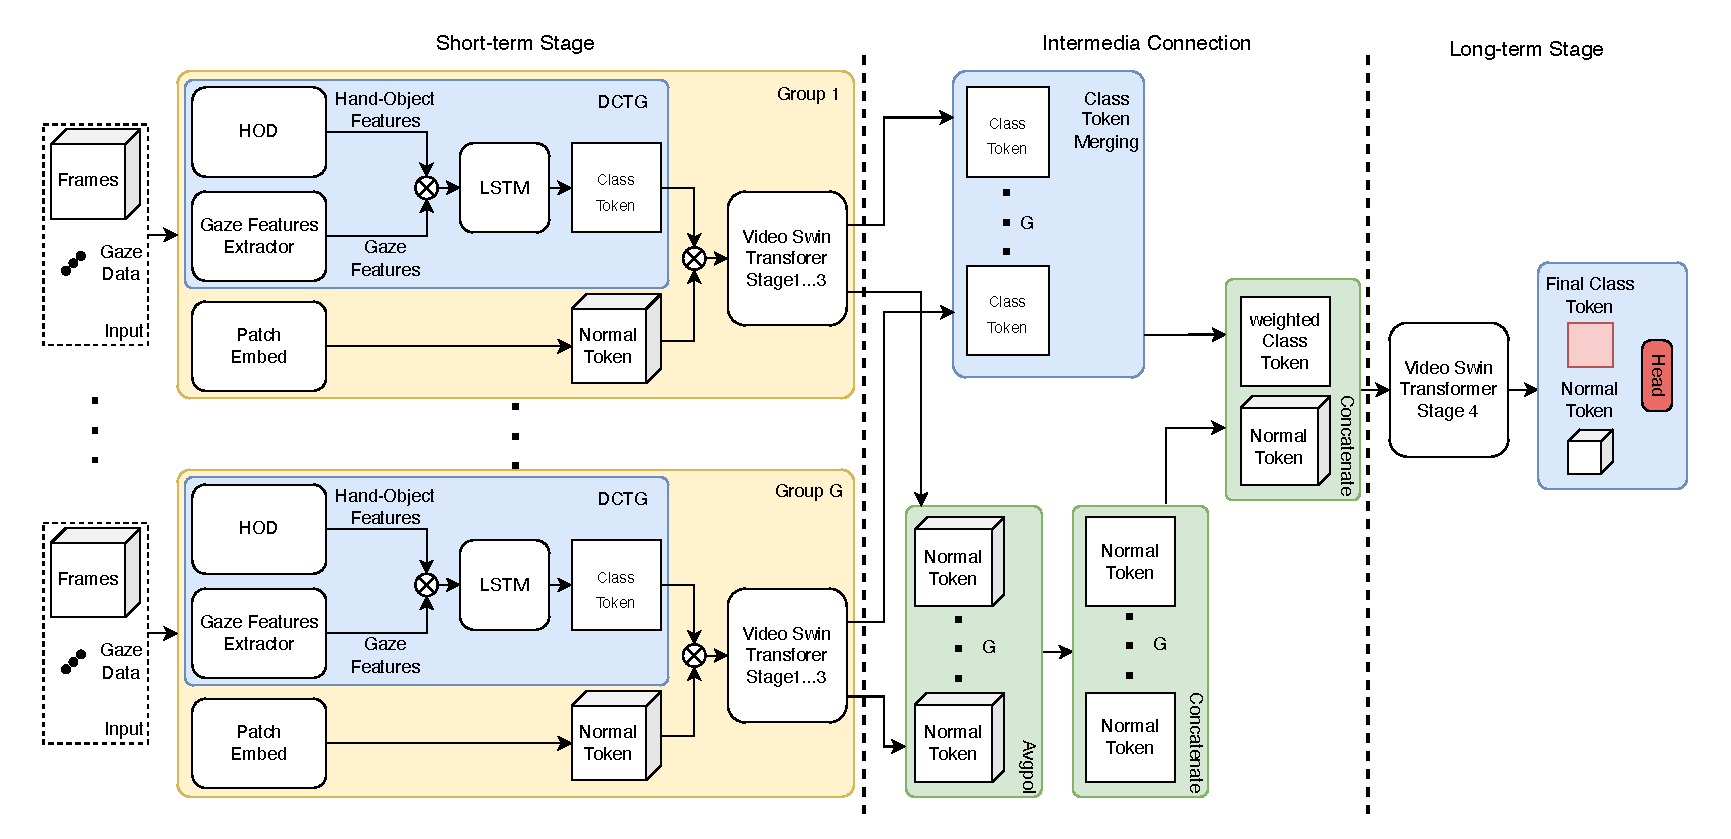
\includegraphics[width=\textwidth]{graphics/structure.pdf}
%         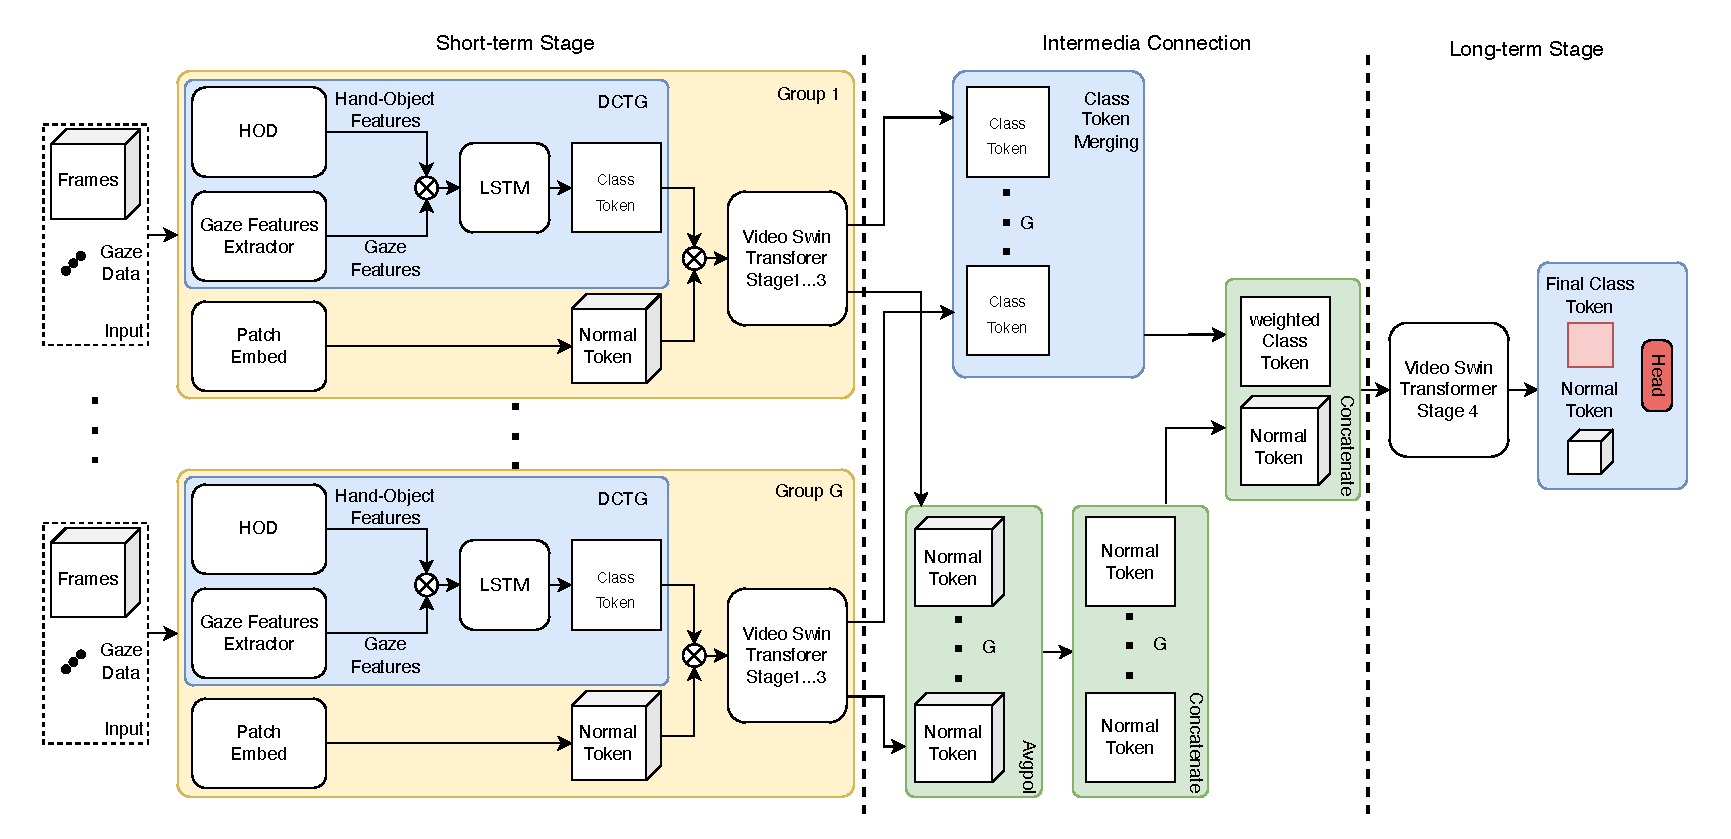
\includegraphics[width=\paperwidth]{graphics/structure.pdf}
%         \caption{The original EgoViT architecture.}
%         \label{fig:ego_vit}
%     \end{figure}
% \end{landscape}

\section{The Gaze-Enhanced DCTG Module}
\label{sec:Gaze-Enhanced DCTG Module}
To integrate gaze information, the Gaze-Enhanced \gls{dctg} module was developed. This module is a key component of the proposed model, responsible for extracting gaze features from the given gaze points and merging them with hand-object features. Finally, a class token is generated from the gaze-hand-object features and fed into subsequent layers. The module consists of three submodules: the Gaze Feature Extractor, the Hand-Object Feature Extractor, and the \gls{lstm} module. The structure of the Gaze-Enhanced \gls{dctg} module is shown in Figure \ref{fig:gaze_dctg}.
\begin{figure}
    \centering
    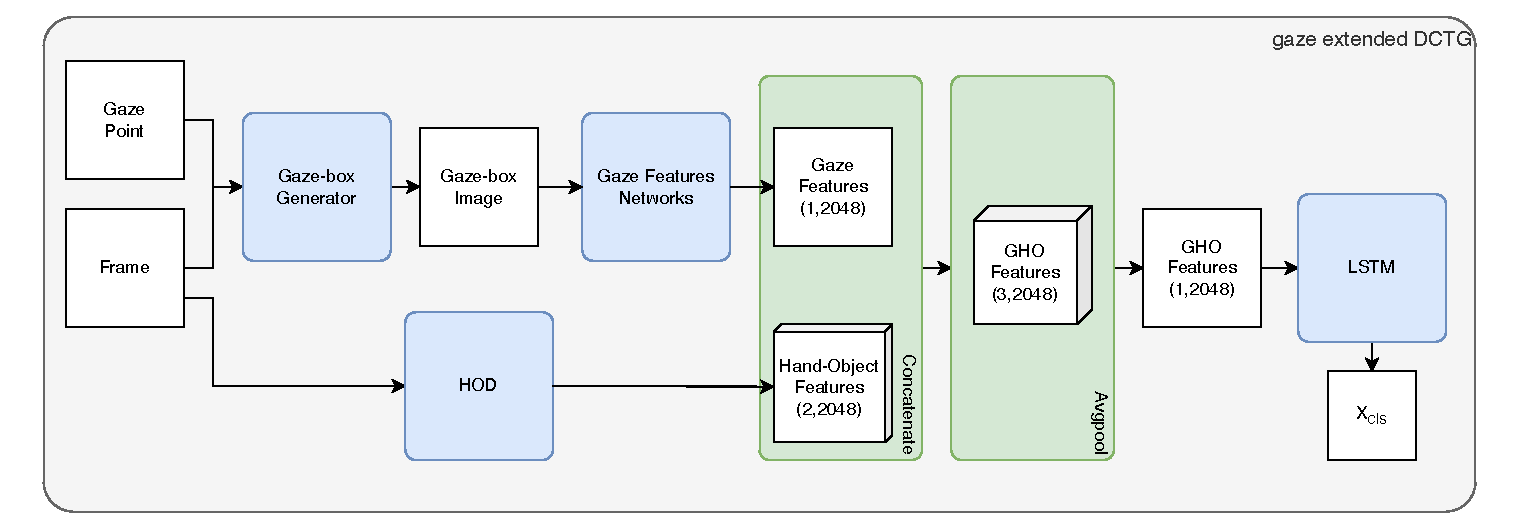
\includegraphics[width=\textwidth]{graphics/dctg.pdf}
    \caption{The data pipeline of the Gaze-Enhanced DCTG module.}
    \label{fig:gaze_dctg}
\end{figure}

The Gaze Feature Extractor is responsible for extracting the gaze features from the given gaze points and frames. The gaze points and frames are first fed into the Gaze-Box Generator. The gaze-box represents the region of the gaze area in the frame, with the gaze point being the center of the gaze region. A square box of size $35 \times 35$ is generated. Based on the gaze-box, a gaze image is cropped from the frame. The gaze image is then fed into the Gaze Feature Networks to extract the gaze features. The $T$ frames and their associated gaze points are sent to the Gaze-Enhanced \gls{dctg}, and the input of the Gaze Feature Networks can be denoted as $I^{gb} \in \mathbb{R}^{T \times 35 \times 35 \times C}$,  where "gb" stands for gaze-box.

The Gaze Feature Networks is a convolutional neural network, as shown in Figure \ref{fig:gaze_feature_networks}. The network consists of three convolutional blocks, each containing a convolutional layer, a batch normalization layer, a ReLU activation layer, and a max-pooling layer.  At the end, the gaze features pass through a flatten layer and a linear layer to generate the output in $D$-dimensions. The output of the Gaze Feature Networks is denoted as $I^{gaze} \in \mathbb{R}^{T \times D}$, where $D$ is the dimension of the gaze features.

\begin{figure}
    \centering
    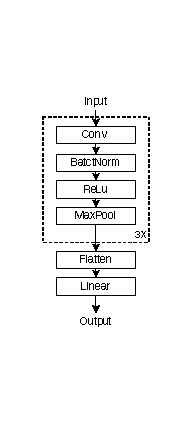
\includegraphics[width=0.5\textwidth]{graphics/gaze_feature_networks.pdf}
    \caption{The structure of the Gaze Feature Networks.}
    \label{fig:gaze_feature_networks}
\end{figure}

A modified \acrlong{hod} module \cite{shan_understanding_2020} is applied offline in this thesis. The \gls{hod} is a pre-trained hand-object detector based on Faster-RCNN networks \cite{ren_faster_2016}. It is designed to detect and classify hands and the objects they interact with in videos. The output consists of the bounding boxes of the hands and objects, as well as their class labels. The code of \gls{hod} is modified to also provide the features of the hands and objects.

Let $I \in \mathbb{R}^{T \times H \times W \times C}$ be the input frames. The \gls{hod} predicts bounding boxes $BB$ for hands and objects,  and a feature map $I^{base}$ is generated by the base part of \gls{hod}. The bounding box predictions are overlapped and, according to the credibility ranking, the top-M hand and top-M object detections with confidence scores $\theta > 0.5$ are chosen. The feature maps, along with the detections, are fed into the “RoIAlign” layers and the “top feature refine” module to generate 2048-dimensional vectors for each detected hand and object.

The hand-object features are denoted as $F^{HO} \in \mathbb{R}^{T \times 2M \times 2048}$, where $2M$ represents the $M$ hand (including left and right) features and $M$ object features. Average pooling is then applied to the $M$ hand features and $M$ object features to generate the final hand-object features, denoted as $I^{HO} \in \mathbb{R}^{T \times 2 \times 2048}$. The hand-object feature extraction process in the Gaze-Enhanced \gls{dctg} module can be described by the following equation:
\begin{equation}
    \begin{aligned}
        &cls_{t}, BB_t = HOD(I_t, \theta_t), \quad \text{for } t \in [1, T] \\[12pt]
        &I_t^{\text{base}} = HOD_{\text{base}}(I_t) \in \mathbb{R}^{1024 \times H^b \times W^b}, \\[12pt]
        &I_t^{\text{align}} = \text{ROIAlign}(I_t^{\text{base}}, BB_t) \in \mathbb{R}^{2M \times 1024 \times H^a \times W^a}, \\[12pt]
        &I_t^{HO} = HOD_{\text{top}}(I_t^{\text{align}}) \in \mathbb{R}^{2M \times 2048}, \\[12pt]
        &F_t^{HO} = \text{AvgPool}(I_t^{HO}) \in \mathbb{R}^{2 \times 2048}, \\[12pt]
        &F^{HO} = [F_1^{HO}, \ldots, F_T^{HO}]  \in \mathbb{R}^{T \times 2 \times 2048}
    \end{aligned}
    \label{eq:hand_object_feature}
\end{equation}
where $I_t$ is the $t$-th frame along temporal axis, $cls_t$ are the class labels of the hands and objects, which are not needed in this thesis. $H^b$ and $W^b$ are the height and width of the feature maps $I_t^{\text{base}}$, $H^a$ and $W^a$ are the height and width of the feature maps $I_t^{\text{align}}$. $M$ is the number of hands and objects detected in each frame.

The extracted gaze features $F^{G} \in \mathbb{R}^{T \times 2 \times 2048}$ and hand-object features $F^{HO} \in \mathbb{R}^{T \times 1 \times 2048}$ are concatenated. Thus, the gaze-hand-object features are denoted as $F^{GHO} \in \mathbb{R}^{T \times 3 \times 2048}$.  The mean value of these three types of features is then calculated as:
\begin{equation}
    \begin{aligned}
        &F^{GHO} = [F^{G}, F^{HO}] \in \mathbb{R}^{T \times 3 \times 2048}, \\[12pt]
        &F^{GHO}_{t} = \frac{1}{3} \sum_{t=1}^{3} F^{GHO}_{t,i}, \quad \text{for } t \in [1, T], \quad i \in [1, 3]
    \end{aligned}
    \label{eq:mean_feature}
\end{equation}
The final gaze-hand-object features are denoted as $F^{GHO} \in \mathbb{R}^{T \times 2048}$. According to \cite{pan_egovit_2023}, applying the \gls{lstm} achievs better performence in aggregating knowledge from the temporal dimension. Therefore, the \gls{lstm} module is applied to generate the class token $x_{cls} \in \mathbb{R}^{T \times D}$ from the gaze-hand-object features $F^{GHO}$. The gaze-hand-object features is projected from 2048-dimensional features to $D$-dimensional features. The \gls{lstm} provided in the pytorch liberary is used in this thesis. The last state of the output of the \gls{lstm} is defined as the class token $x_{cls}$. The procedure for generating the class token can be described as follows:
\begin{equation}
    \begin{aligned}
        &F^{GHO'} = \text{LSTM}([F^{GHO}_1,\ldots , F^{GHO}_T]) \in \mathbb{R}^{T \times D}, \\[12pt]
        &x_{cls} = F^{GHO'}[-1] \in \mathbb{R}^{D}
    \end{aligned}
    \label{eq:class_token}
\end{equation}
where $F^{GHO'}$ is the output of the \gls{lstm} module, and $F^{GHO'}[-1]$ is the last state of the output along the temporal axis.

\section{Integration of Video Swin Transformer}
\label{sec:Integration of Video Swin Transformer}
The Video Swin Transformer is used as the backbone in both the short-term and long-term stages, separated by the Dynamic Merging module. The Video Swin Transformer is modified to fit the architecture of the Gaze-Enhanced EgoViT by dividing it into two parts. The PatchEmbedding layers and stages 1 to 3 are in the short-term stage, responsible for extracting local temporal information. Stage 4 is in the long-term stage, responsible for extracting global temporal information. The configuration of the Video Swin Transformer follows the Swin-B model in \cite{liu_video_2021}.

The structure of the Video Swin Transformer in the short-term stage is shown in Figure \ref{fig:video_swin_transformer}. The 3D local window is defined as $WI \in \mathbb{R}^{WI_T \times WI_H \times WI_W}$. The patches are denoted as $X^P \in \mathbb{R}^{T_P \times H_P \times W_P \times D}$, where $T_{WI} = \frac{T_P}{WI_T}$, $H_{WI} = \frac{H_P}{WI_H}$, and $W_{WI} = \frac{W_P}{WI_W}$. There are a total of $N_{WI} = T_{WI} \times H_{WI} \times W_{WI}$ windows. Unlike a classic vision transformer, the Video Swin Transformer does not use the class token as the first token in the sequence. Instead, the normal token from 3D shifted windows is used to aggregate information. Therefore, the dimension of the class token in the Gaze-Enhanced EgoViT is expanded to assign the same class token to all 3D windows. After the assignment, each 3D window has a class token and updates it independently.
\begin{figure}
    \centering
    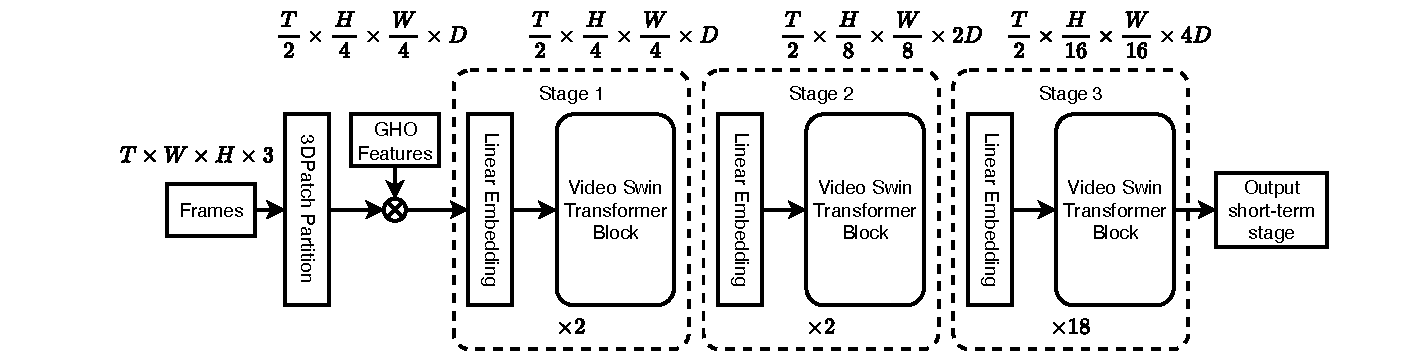
\includegraphics[width=\textwidth]{graphics/vst_st.pdf}
    \caption{The structure and the data pipeline of the short-term stage.}
    \label{fig:video_swin_transformer}
\end{figure}

The input to stage 1 is denoted as:
\begin{equation}
    \begin{aligned}
    &I_{WI,i} = [x_{cls,i}, x_{WI,i}] \quad i \in [1, N_{WI}], \\[12pt]
    &I_{WI,i} \in \mathbb{R}^{((1 + WI_T) \times WI_H \times WI_W) \times D}
    \end{aligned}
\end{equation}
where $i$ denotes the $i^{th}$ window and $x_{WI,i}$ is the normal token of the $i^{th}$ window.

The operation of the dynamic class token in a transformer block is expressed in the following equation:
\begin{equation}
    \begin{aligned}
        \hat{I}_{WI,i}^l &= \text{W-MSA}(\text{LN}(I_{WI,i}^{l-1})) + I_{WI,i}^{l-1}, \\[10pt]
        I_{WI,i}^l &= \text{MLP}(\text{LN}(\hat{I}_{WI,i}^l)) + \hat{I}_{WI,i}^l, \\[10pt]
        \hat{I}_{WI,i}^{l+1} &= \text{SW-MSA}(\text{LN}(I_{WI,i}^l)) + I_{WI,i}^l, \\[10pt]
        I_{WI,i}^{l+1} &= \text{MLP}(\text{LN}(\hat{I}_{WI,i}^{l+1})) + \hat{I}_{WI,i}^{l+1},
    \end{aligned}
\end{equation}
Where LN refers to Layer Normalization, (S)W-MSA refers to the (shifted) Windowed Multi-head Self-Attention, and MLP refers to the Multi-Layer Perceptron. $\hat{I}_{WI,i}^{l}$ and $I_{WI,i}^l$ are the output of (S)W-MSA and MLP in the $l^{th}$ block, respectively. 

The class tokens are attached to the first position in the temporal dimension of the 3D windows.  This produces a hierarchical representation similar to the Video Swin Transformer. The class token neighborhoods within a $2 \times 2$ spatial space are concatenated, which downsamples the spatial dimension by a factor of 2 and increases the $D$-dimensional features by a factor of 4. A linear layer is then applied to project the features to half of their dimension. For example, the output of stage 1 is $\frac{T}{2} \times \frac{H}{4} \times \frac{W}{4} \times D$, then after the Linear Embedding and Transformer Block, the output of the stage 2 becomes $\frac{T}{2} \times \frac{H}{8} \times \frac{W}{8} \times 2D$. Note that downsampling is not applied in the temporal dimension.

\begin{figure}[t]
    \centering
    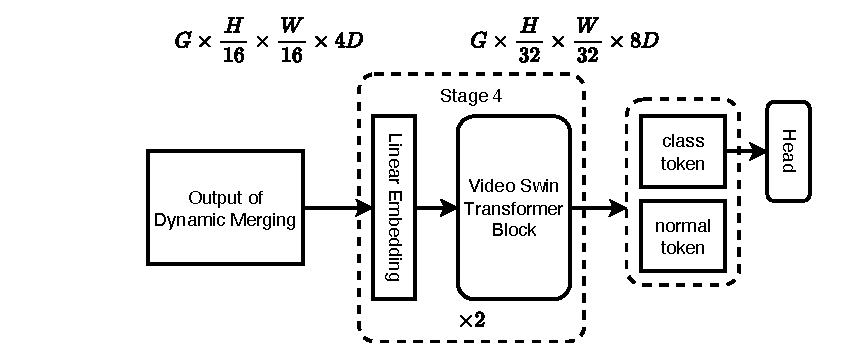
\includegraphics[width=0.9\textwidth]{graphics/vst_lt.pdf}
    \caption{The structure the data pipeline of long-term stage.}
    \label{fig:video_swin_transformer_lt}
\end{figure}

Therefore, the proposed model combines the characteristics of the shifted Window Multi-head Self-Attention and the EgoViT architecture. The shifted Window Multi-head Self-Attention exchanges information in the spatial dimension, while each group in the short-term stage of EgoViT exchanges information in the local temporal dimension. 

The long-term stage consists of the stage 4 of the Video Swin Transformer. The structure and goal of this stage follow the approach in \cite{pan_egovit_2023}, aiming to perceive actions over long durations by exploring the inter-relationships established in the short-term stage. The input tensor $x_{mrg}$ to stage 4 is the concatenation of the weighted class token $x^{cls}_{mrg}$ and the normal token $x^{P}_{mrg}$, which is expressed as:
\begin{equation}
    x_{merge} = [x^{cls}_{mrg}, x^{P}_{mrg}] \in \mathbb{R}^{(1 + G) \times \frac{H}{16} \times \frac{W}{16} \times 4D}
\end{equation}
Figure \ref{fig:video_swin_transformer_lt} shows the structure of the Video Swin Transformer in the long-term stage. After processing in stage 4, the output is separated into two parts: the class token $x^{cls}_{lt} \in \mathbb{R}^{1 \times H^{s4}_{wi} \times W^{s4}_{wi} \times 4D}$ and the normal token $x^{P}_{lt} \in \mathbb{R}^{G \times \frac{H}{32} \times \frac{W}{32} \times 4D}$, where the subscript “lt” denotes the long-term stage, and $H^{s4}_{wi}$ and $W^{s4}_{wi}$ are the height and width of the window in stage 4. Only the class token is fed into the Head to calculate the score for each action class. The Head consists of a sequence of layers, including an Average Pooling layer, a Flatten layer, and a Linear layer, which together transform the class token from 2048-dimensional features to a score between 0 and 1, representing the final score for each action class. 

\section{Dynamic Merging Module}
\label{sec:Dynamic Merging Module}
\begin{figure}[b]
    \centering
    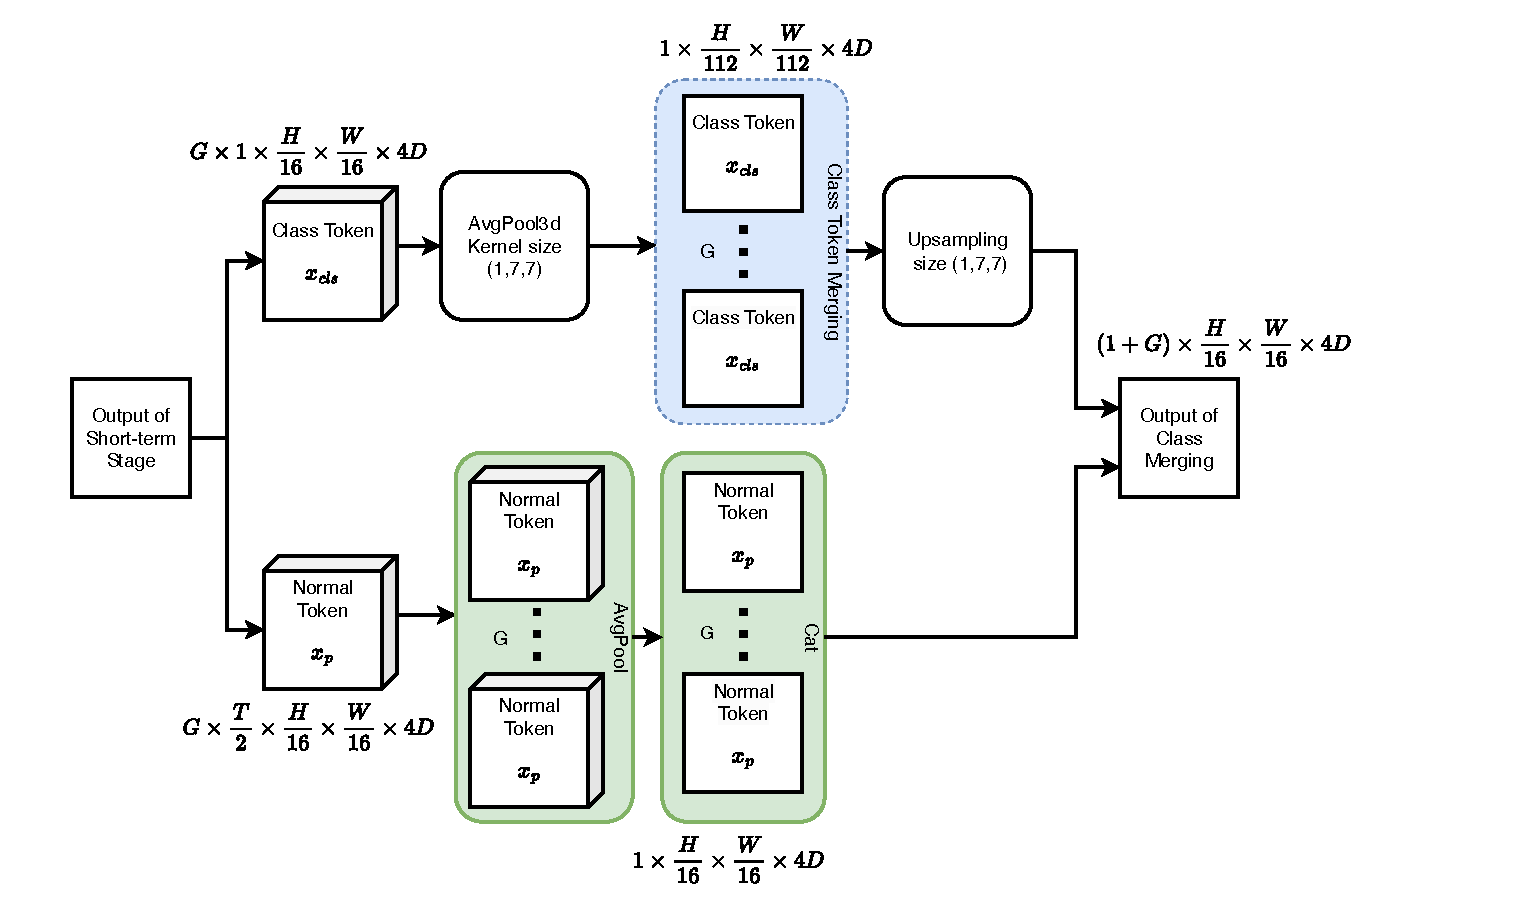
\includegraphics[width=\textwidth]{graphics/dm.pdf}
    \caption{The structure of the Dynamic Merging module.}
    \label{fig:dynamic_merging}
\end{figure}
% \vspace{5mm}
After being processed in the short-term stage, the class token serves as a summary of the short-term actions. The Dynamic Merging module is designed to assign a larger weight to the class tokens representing key short-term actions \cite{pan_egovit_2023}. The structure of the Dynamic Merging module is shown in Figure \ref{fig:dynamic_merging}. The input tensor is $x_{st} \in \mathbb{R}^{G \times (1+\frac{T}{2}) \times \frac{H}{16} \times \frac{W}{16} \times 4D}$. Before merging, the class token $x_{cls}$ and the normal token $x_{P}$ are separated. The class token $x_{cls}$ from each group are fed into an AvgPool3d layer to obtain the class token for each 3D window. According to the window size of the Video Swin Transformer (2, 7, 7), the kernel size of AvgPool3d is set to (1, 7, 7). Then the weighted class token $x^{cls}_{mrg}$ is calculated from the $G$ downsampled class tokens.

The merging algorithm is expressed in Equation \ref{eq:x_cls_s}. First, the dot product between the class tokens of different groups is calculated. The score $\alpha_{g,s,g'}$ is the dot product divided by their l2 norms. The total score $\alpha_{g,s}$ for $x^{cls}_{g,s}$ is calculated by summing the scores along the spatial and group axes. The scores for all class tokens are normalized along the group axis using the softmax operator. The weighted class token $x^{cls}_{mrg}$ for the lont-term stage is then obtained by computing the weighted sum of class tokens along the group axis. Finally, the weighted class token is sent to an upsampling layer with size (1, 7, 7) to match the size of $1 \times \frac{H}{16} \times \frac{W}{16} \times 4D$.

An AvgPool layer is first applied to the $G$ normal tokens $x_{P}$ along the temporal axis, and then the $G$ normal tokens are concatenated to form the normal token with a shape of $G \times \frac{H}{16} \times \frac{W}{16} \times 4D$. At the end of this module, the class token $x^{cls}_{mrg}$ and the normal token $x^{P}_{mrg}$ are concatenated to form the input tensor $x_{lt} \in \mathbb{R}^{(1+G) \times \frac{H}{16} \times \frac{W}{16} \times 4D}$ for the long-term stage. 
\chapter{Experiments and Results}
\label{chap:experiments}
In this chapter, the experiment setup and results are described in detail. In section \ref{sec:setup}, the datasets, developing environment, metrics, and implementation details are explained. Section \ref{sec:training_original_egovit} presents the results of the original EgoViT on the EGTEA Gaze+ dataset. In Section \ref{sec:training_egovit_with_gaze}, the results of the enhanced EgoViT training with gaze information are presented. Finally, the results of the experiments are analyzed and discussed in Section \ref{sec:Disscussion}.

% In this chapter, we describe the experimental setup and the results of our experiments. We start by describing the experimental setup in Section~\ref{sec:setup}. Then, we present the results of training the original EgoViT model on the EGTEA Gaze+ dataset in Section~\ref{sec:training_original_egovit}. In Section~\ref{sec:training_egovit_with_gaze}, we present the results of training the EgoViT model with gaze information.

\section{Setup}
\label{sec:setup}
\textbf{Datasets} The largest commonly used egocentric video dataset is EPIC-KITCHENS \cite{Damen2018EPICKITCHENS}, which contains videos of daily activities from multiple participants in their natural environment. However, this dataset does not provide gaze data from the videos. For this reason, the EGTEA Gaze+ \cite{li_eye_2020} dataset is utilized in this thesis. EGTEA Gaze+ is a large and comprehensive dataset for \gls{fpv} actions and gaze tracking. It includes HD videos, gaze tracking data, and frame-level action annotations. The dataset consists of 86 unique sessions from 32 subjects across 7 recipes. The annotations include 10321 action instances from 106 action categories, with an average action instance duration of 4.2 seconds. There are three non-overlapping train and test sets available, with 8299/2022, 8299/2022 and 9230/2021 samples (train/test). These splits are generated through random sampling, ensuring that approximately  80\% of the samples per category are included. The split set 1 is used in this thesis for training and testing. For all Experiments, this study follows prior work by reporting top-1 accuracy, top-5 accuracy and average mean class accuracy.

\textbf{Developing Environment} The experiments are conducted on a GPU server in SimTech Stuttgart. The server runs Ubuntu operating system, and the model with its experiments are implemented in Python 3.9. The deep learning framework PyTorch 2.2 and CUDA 12.1 are used for the implementation.
The important ependencies and their versions are listed below:
\begin{itemize}
    \item torch==1.10.0
    \item torchvision==0.17.0
    \item numpy==1.26.4
    \item pandas==2.2.1
    \item opencv-python==4.10.0.82 
\end{itemize}

\textbf{Implementation Details} The video clips in  EGTEA Gaze+ dataset have an average length of 3.2 seconds, although some clips are significantly longer. To handle this, the video clips are uniformly sampling into 32 frames. The frames are resized to $224 \times 224$ pixels, resulting in an input tensor of shape $32 \times 3 \times 224 \times 224$. Dimension 3 represents the RGB channels of the image. Another input tensor contains gaze tracing data with a shape of $32 \times 1 \times 1$, where $1 \times 1$ represents gaze coordinates $(x,y)$in each frame. The gaze coordinates are normalized to the range of $[0, 1]$. 

Frame extraction from the video clips and the processing of gaze features can be time-consuming during training. To reduce the training time, frame extraction and gaze-hand-object features processing are performed offline and saved as a NumPy zipped (.npz) file. And the action label is also read and saved in this zipped file. Thus, the image, gaze-hand-object features, and action label of one video clip are saved in a single file. The structure of the NumPy zipped (.npz) file is as follows:
\begin{align*}
    \text{Preprocessed Data:} & (\text{frames}: [32, 3, 224, 224], \quad \text{features}: [32, 3, 2048], \quad \text{label}: [1])
\end{align*}
The training process opens the data file only once for each video clip, significantly reducing the training time. All experiments are conducted on the prepared data.

The models are trained using the AdamW \cite{loshchilov_decoupled_2019} optimizer.  The learning rate is set to $1 \mathrm{e}{-5}$, and the batch size is set to 4. The layers the in Video Swin Transformer use the pretrained weights from KINETICS400\_V1. The models are trained for 20 epochs. In some experiments, a cosine decay learning rate scheduler with a linear warm-up of 2.5 epochs is used, following the approach in \cite{liu_video_2021}. The stochastic depth rate and weight decay are adopted as in \cite{liu_video_2021}, set to 0.3 and 0.05 respectively. The configuration of Swin-B is used. The architecture hyperparameters of Swin-B are as follows:
\begin{align}
    \text{Swin-B:} &\quad C = 128, \quad \text{layer numbers} = \{2, 2, 18, 2\}
\end{align}
Where $C$ represents the $C$-dimentional features (see Figure \ref{fig:swin-transformer}), and $\{2, 2, 18, 2\}$ represents the number of times the Transformer Block is repeated in each stage.

\textbf{Metrics} For inference, the same data structure as used in training is applied. The model is evaluated on the test split1 of the EGTEA Gaze+ dataset. The top-1 accuracy, top-5 accuracy, and mean class accuracy are calculated. The top-1 accuracy is the proportion of correctly predicted class (with the highest predicted probability) among all samples. It is the most straightforward accuracy metric. The calculation of top-1 accuracy is:
\begin{align}
    \text{Top-1 Accuracy} = \frac{\text{Number of correctly predicted samples}}{\text{Total number of samples}}
\end{align}
Top-5 accuracy refers the percentage of instances where the true class label is within the top five predicted class label. The formula for top-5 accuracy is:
\begin{align}
    \text{Top-5 Accuracy} = \frac{\text{Number of correctly predicted samples in top-5}}{\text{Total number of samples}}
\end{align}
The mean class accuracy is the average accuracy for each class. It accounts class imbalance by assigning equal weight to each class. The formula for mean class accuracy is:
\begin{align}
    \text{Mean Class Accuracy} = \frac{1}{N} \sum_{i=1}^{N} \frac{\text{Number of correctly predicted samples for class i}}{\text{Total number of samples in class i}}
\end{align}
Where $N$ is the number of classes. 
\clearpage
In this thesis, a series number of experiments are conducted. Different models are trained with different features and configurations. For a simple discription of the experiments, the experiments ID are denoted and explained in the Table \ref{tab: exp_id}. The experiments ID are used to identify the experiments in the following sections. When not mentioned, the experiments are trained with gaze version 1, with pretrained weights from KINETICS400\_V1, and a fixed learning rate of $1 \mathrm{e}{-5}$.
\vspace{5mm}
\begin{table}[htbp]
    \centering
    \caption{Experiments ID and Description}
    \begin{tabular}{ll}
    \hline\hline
    Experiment ID & Description \\
    \hline
    Orig\_HO\_no\_pretrain  & Original EgoViT: without pretrained weights \\
    Orig\_HO                & Original EgoViT: pretrained weights \\
    Orig\_HO\_sched. LR     & Original EgoViT: pretrained weights and scheduler LR \\
    Enh\_GHO             & Enhanced EgoViT: GHO features \\
    Enh\_G               & Enhanced EgoViT: G features \\
    Enh\_GHO\_v2         & Enhanced EgoViT: GHO features and gaze\_v2 \\
    Enh\_G\_v2           & Enhanced EgoViT: G features and gaze\_v2 \\
    Enh\_v2\_GHO\_v2     & Enhanced EgoViT\_v2: GHO features and gaze\_v2 \\
    Enh\_v3\_HO          & Enhanced EgoViT\_v3: HO features \\
    Enh\_v3\_GHO\_v2     & Enhanced EgoViT\_v3: GHO features and gaze\_v2 \\
    Enh\_v3\_G\_v2       & Enhanced EgoViT\_v3: G features and gaze\_v2 \\
    \hline\hline
    \end{tabular}
    \label{tab: exp_id}
\end{table}
\clearpage


\section{Training the Original EgoViT with EGTEA Gaze+ Dataset}
\label{sec:training_original_egovit}
Because the code for the original EgoViT is not publicly available, an approximate model is first built in this thesis. To compare the effect of gaze information, the original EgoViT from \cite{pan_egovit_2023} is trained on the EGTEA Gaze+ dataset and used as the baseline for all experiments. Therefore, only frames and hand-object features in the video clips are fed into the original EgoViT model.

The original EgoViT model is first trained without pretrained weights from KINETICS400\_V1, using a learning rate of $1 \mathrm{e}{-5}$ for all layers. The model is trained for 40 epochs. Figure \ref{fig:orig-EgoViT} shows the training loss and accuracy of the original EgoViT model. The rot line represents the training loss, and the blue line represents the training accuracy. The model converges rapidly in the first 5 epochs and the loss decreases consistently between 5 and 30 epochs. After 30 epochs, the model converges slowly to the minimum loss. The accuracy follows a similar trend, inversely related to the loss.

\begin{figure}[b]
    \centering
    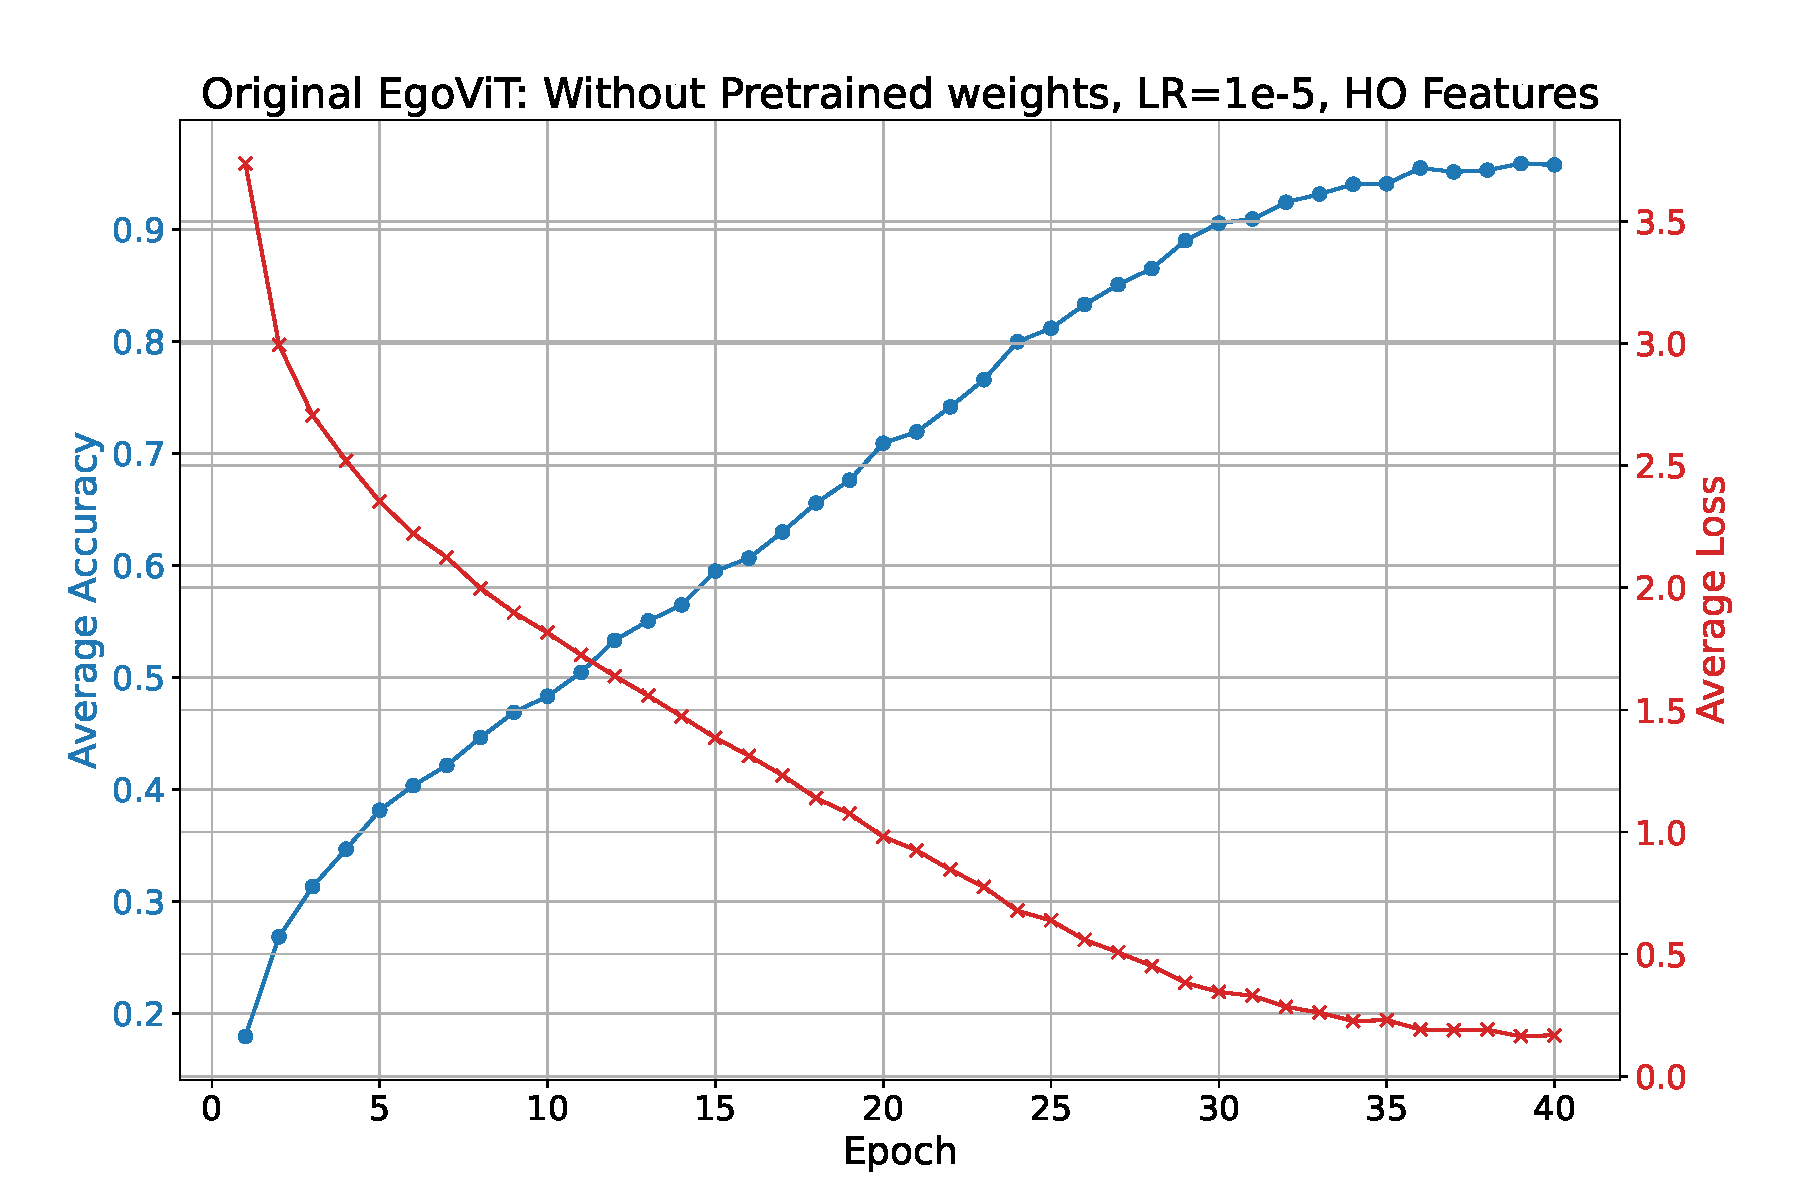
\includegraphics[width=0.9\textwidth]{graphics/figure11}
    \caption{The training loss and accuracy curves for the original EgoViT model trained without pretrained weights. The model is trained over 40 epochs with a learning rate of 1e-5. Blue curve: training accuracy, red curve: training loss.}
    \label{fig:orig-EgoViT}
\end{figure}
\clearpage
\begin{figure}[htbp]  
    \centering
    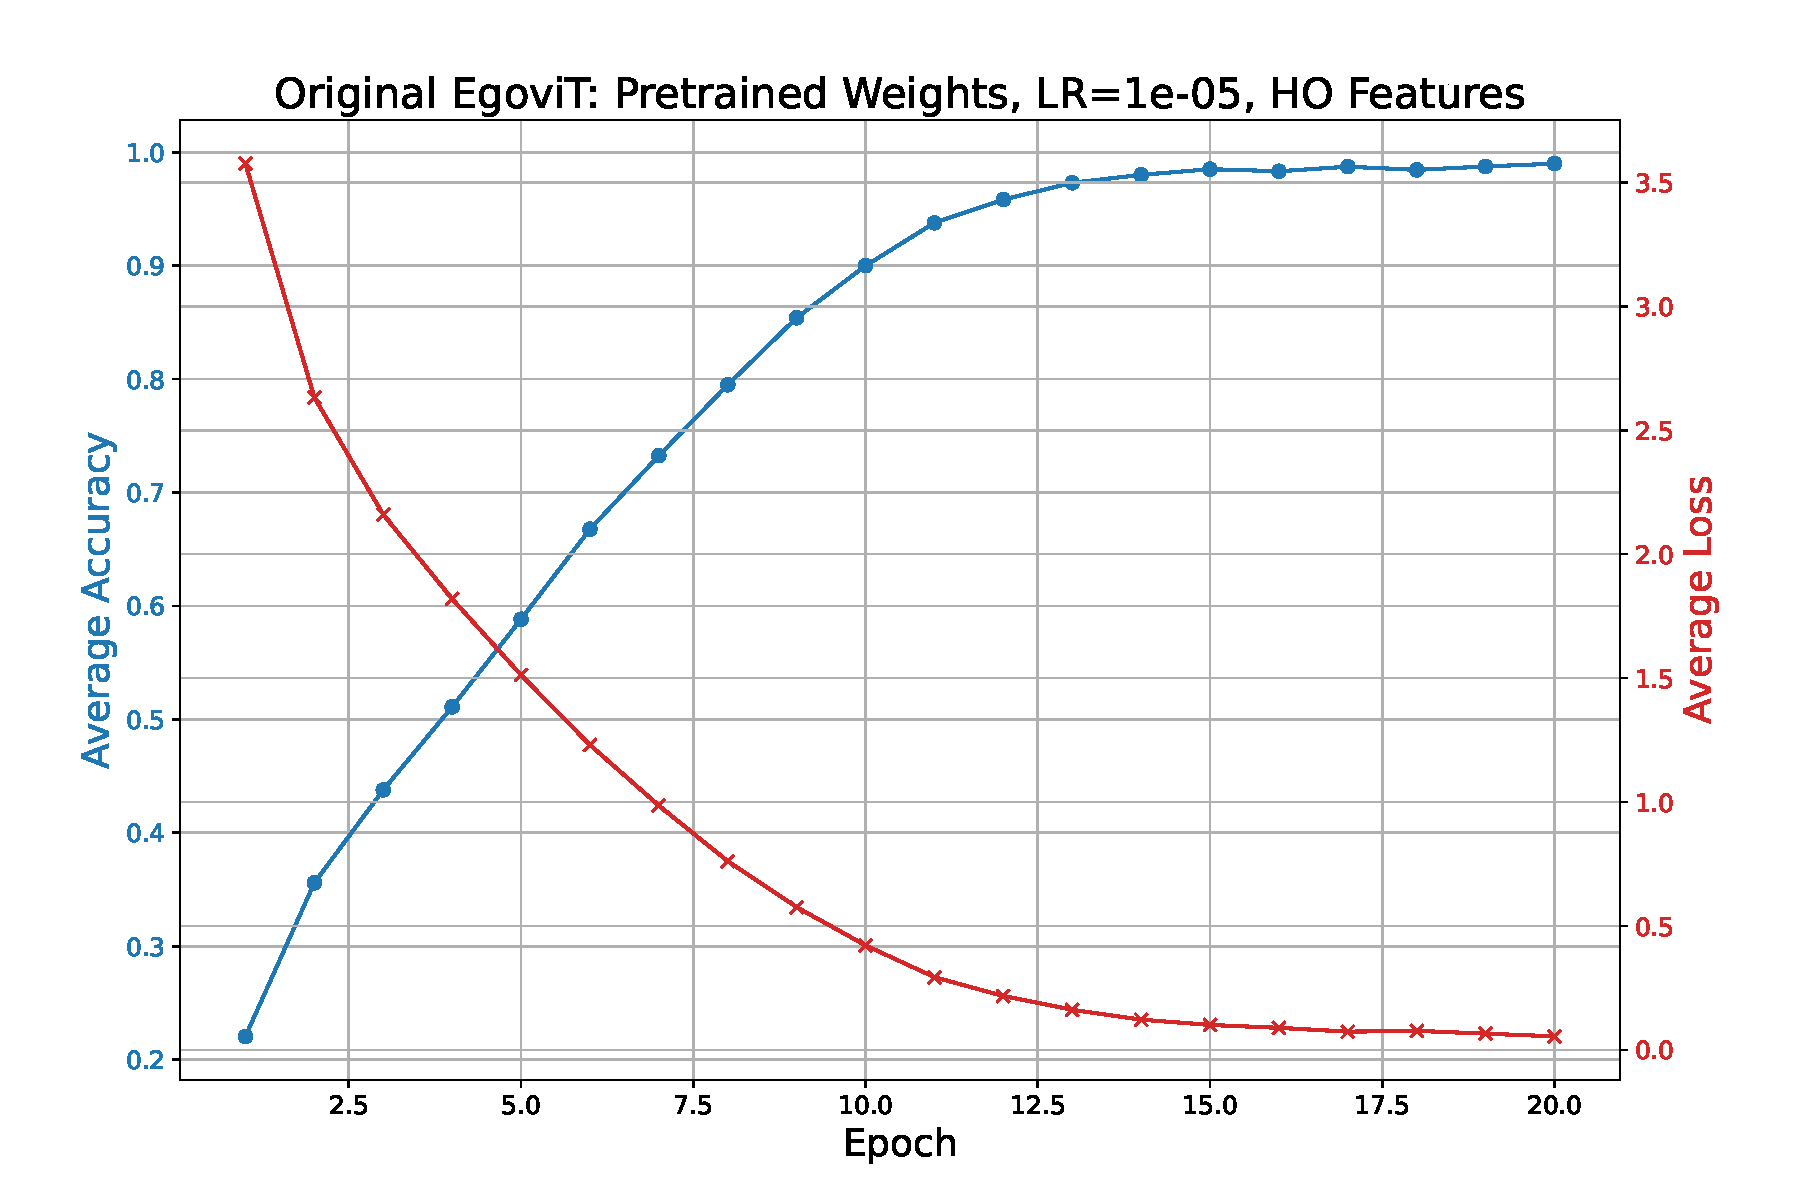
\includegraphics[width=0.9\textwidth]{graphics/figure31}
    \caption{The training loss and accuracy curves for the original EgoViT model trained with pretrained weights. The model is trained over 20 epochs with a learning rate of 1e-5. Blue curve: training accuracy, red curve: training loss.}
    \label{fig:orig-EgoViT-with-pretrained}
\end{figure}
\vspace{3mm}
To improve the training performance, the original EgoViT model is trained with pretrained weights from KINETICS400\_V1, while maintaining a learning rate of $1 \mathrm{e}{-5}$. The model is trained for 20 epochs. Figure \ref{fig:orig-EgoViT-with-pretrained} shows the training loss and accuracy of the original EgoViT model with pretrained weights. The loss decreases rapidly in the first 3 epochs and then follows a shorter, consistently decreasing period. After 20 epochs, the model converges slowly to the minimum loss. The accuracy follows a similar trend, inversely related to the loss. By the 13th epoch, the model is almost fully converged and then decreases slowly to the minimum. This result indicates that the model with pretrained weights performs better than the model without them. Therefore, in the following experiments, the model with pretrained weights is used.

\clearpage
\begin{figure}[htbp]
    \centering
    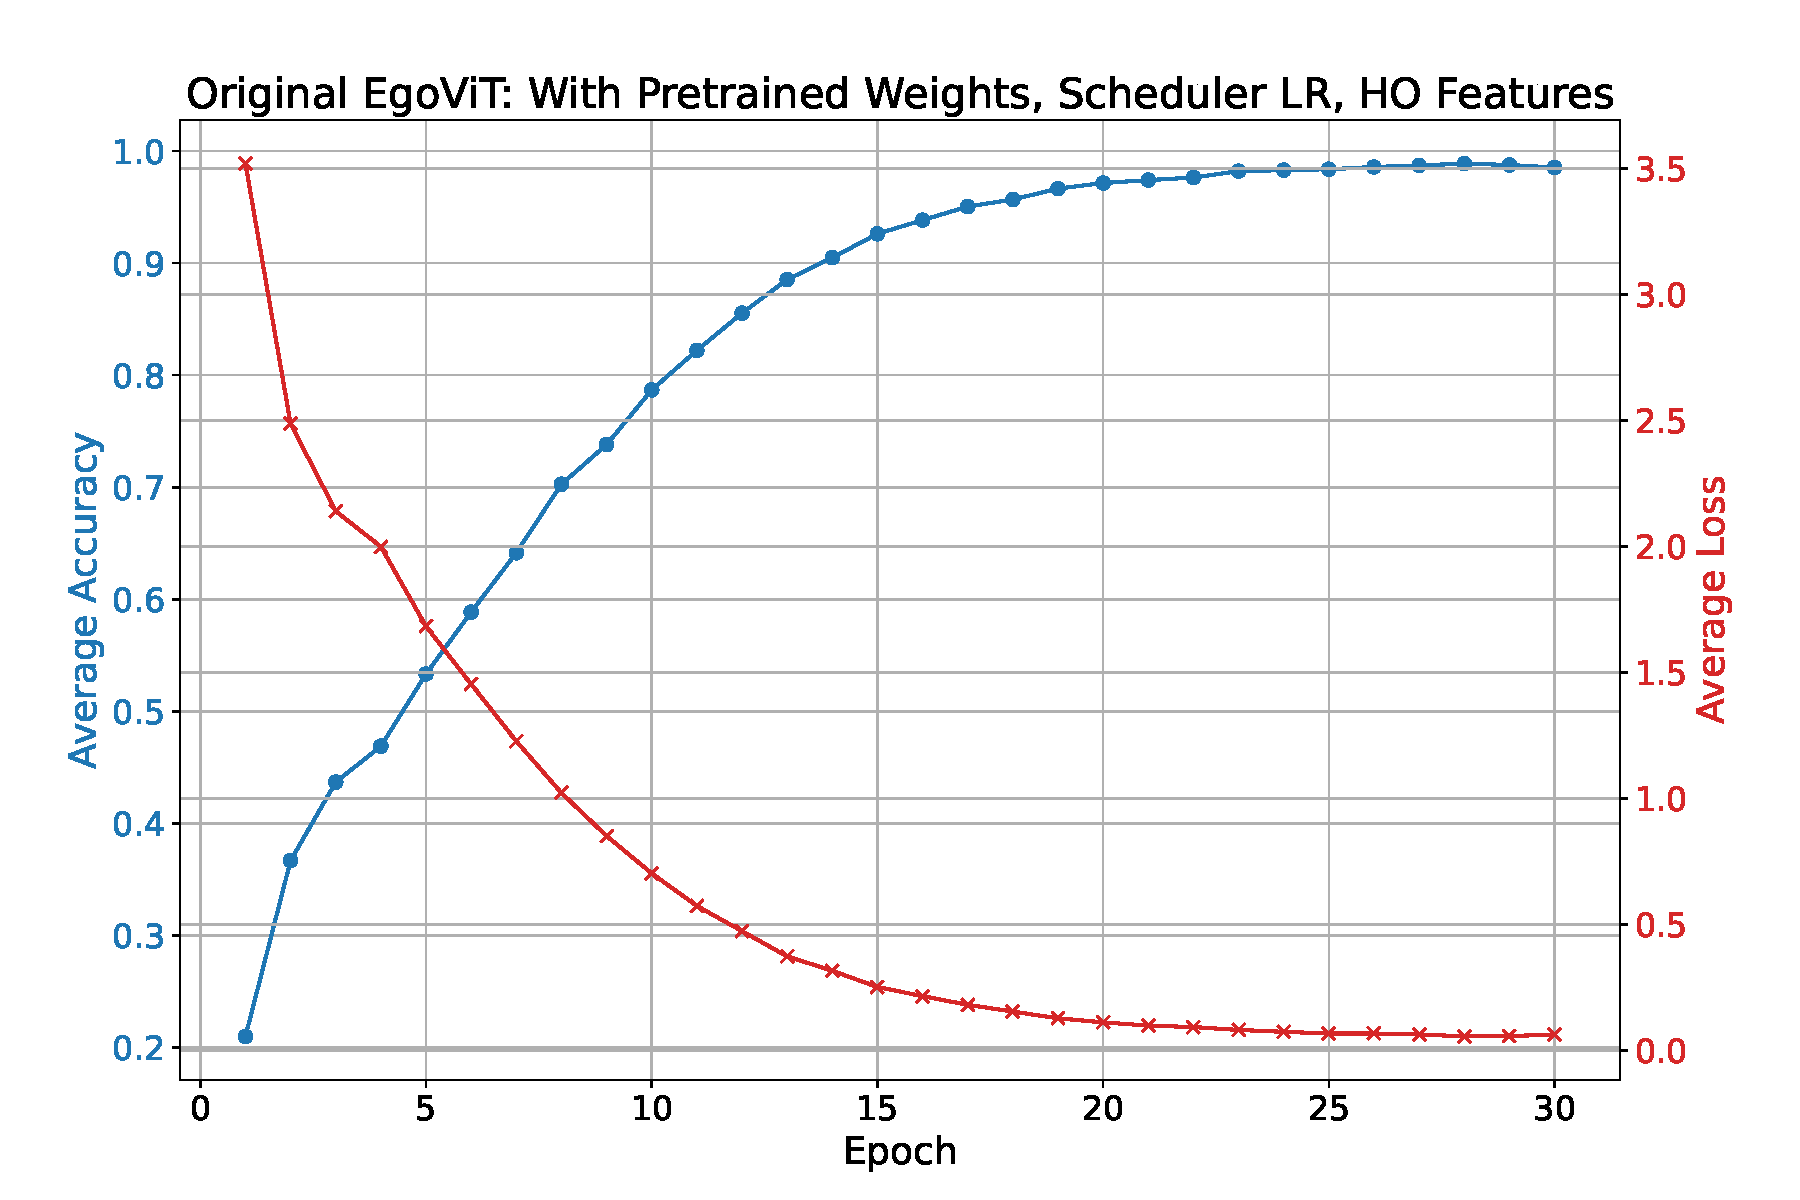
\includegraphics[width=0.9\textwidth]{graphics/figure21}
    \caption{The training loss and accuracy curves for the original EgoViT model trained with pretrained weights. The model is trained over 30 epochs with a scheduler learning rate. Blue curve: training accuracy, red curve: training loss.}
    \label{fig:orig-EgoViT-no-pretrained}
\end{figure}
\vspace{3mm}
The learning rate is another hyperparameter that affects model performance. A cosine scheduler learning rate, as described in \cite{liu_video_2021}, is applied to fine-tune the learning rate. The model is trained for 30 epochs. Figure \ref{fig:orig-EgoViT-no-pretrained} shows the training loss and accuracy of the original EgoViT model with pretrained weights and scheduler learning rate. In the first 10 epochs, the loss decreases rapidly. After 15 epochs, the model converges slowly to the minimum loss. Between 20 and 25 epochs, the model achieves maximum accuracy and minimum loss.

\clearpage
The testing results of three training methods are shown in Table \ref{tab:original-egovit}. The model with pretrained weights and a scheduler learning rate achieves the highest top-1 accuracy of 0.517, followed by the model with pretrained weights and a fixed learning rate of 0.515. The model with pretrained weights and a scheduler learning rate has the worst performance, achieving the lowest top-1 accuracy, top-5 accuracy, and mean class accuracy of 0.484, 0.744, and 0.358, respectively. All three metrics follow a similar trend, with the model using a fixed learning rate of $1 \mathrm{e}{-5}$ showing better performance overall. While the pretrained weights from KINETICS400\_V1 did not improve \gls{ear} in inference, they accelerated the training process. One possible reason for the lower performance of the scheduler learning rate is that the Video Swin Transformer is divided into two parts and the model has many additional, making the scheduler learning rate configuration from \cite{liu_video_2021} potentially unsuitable for the original EgoViT model. A new configuration for the scheduler learning rate could be explored in future work.
\newline

\begin{table}[h]
    \centering
    \caption{Test Results of original EgoViT with HO Features}
    \begin{tabular}{lccc}
    \hline\hline
    Experiment ID & Top-1 Acc.(\%) & Top-5 Acc.(\%) & Mean Class Acc.(\%) \\
    \hline
    Orig\_HO\_no\_pretrain       & 51.5 & 78.5 & 38.8 \\
    Orig\_HO                     & 51.7 & 75.2 & 40.6 \\
    Orig\_HO\_sched. LR          & 48.4 & 74.4 & 35.8 \\
    \hline\hline
    \end{tabular}
    \label{tab:original-egovit}
\end{table}

\section{Training the Enhanced EgoViT with Gaze Information}
\label{sec:training_egovit_with_gaze}
In this section, the enhanced EgoViT is trained with additional gaze information using different methods to evaluate the effect of gaze information on the model. In this series of experiments, two types of gaze data are used for training and testing. The first type, referred to as gaze version 1, contains only the gaze tracking type of fixation. Thus, some sampled frmes may not have gaze data. The second type, referred to as gaze version 2, includes both fixation and saccade types of gaze tracking. Gaze version 2 has more collected gaze data from the dataset but also includes some frames that lack gaze data. For these frames, the missing gaze data is ignorded and gaze features are randomly generated, resulting in a highter overall quality of gaze data compared to gaze version 1.

For an ablation study, the enhanced EgoViT is trained with gaze-hand-object features and only gaze features seperetly. The model is trained for 20 epochs with a learing rate of $1 \mathrm{e}{-5}$. The training loss and accuracy of the enhanced EgoViT model with gaze-hand-object features and gaze features are shown in Figure \ref{fig:egovit-with-gho} and \ref{fig:egovit-with-gaze}. The both training have a similar loss and accuracy curved line compared with the experiment orig\_pretrain\_HO in Figure \ref{fig:orig-EgoViT-with-pretrained}. The three experiments have similarity loss converge rate and all reach the minimum loss after 15 epochs. The top-1, top-5 and mean class accuracy of the two experiments are shown in Table \ref{tab:Results_table2}. The model with hand-object features achieves the highest top-1 accuracy of 0.517 and the highest mean class accuracy of 0.406, followed by the model with gaze-hand-object features, which achieves 0.514 and 0.400, respectively. However, the gaze-hand-object model has the highest top-5 accuracy of 0.767. The model with only gaze features has the lowest scores across all three metrics, with a top-1 accuracy of 0.489, a top-5 accuracy of 0.751, and a mean class accuracy of 0.377. \newline
\begin{table}[h]
    \centering
    \caption{Test Results on Models with Different Features}
    \begin{tabular}{lccc}
    \hline\hline
    Experiment ID & Top-1 Acc. & Top-5 Acc. & Mean Class Acc. \\
    \hline
    Orig\_HO        & 51.7 & 75.2 & 40.6 \\
    Enh\_GHO     & 51.4 & 76.7 & 40.0 \\
    Enh\_G       & 48.9 & 75.1 & 37.7 \\
    \hline\hline
    \end{tabular}
    \label{tab:Results_table2}
\end{table}

% \clearpage
\begin{figure}
    \centering
    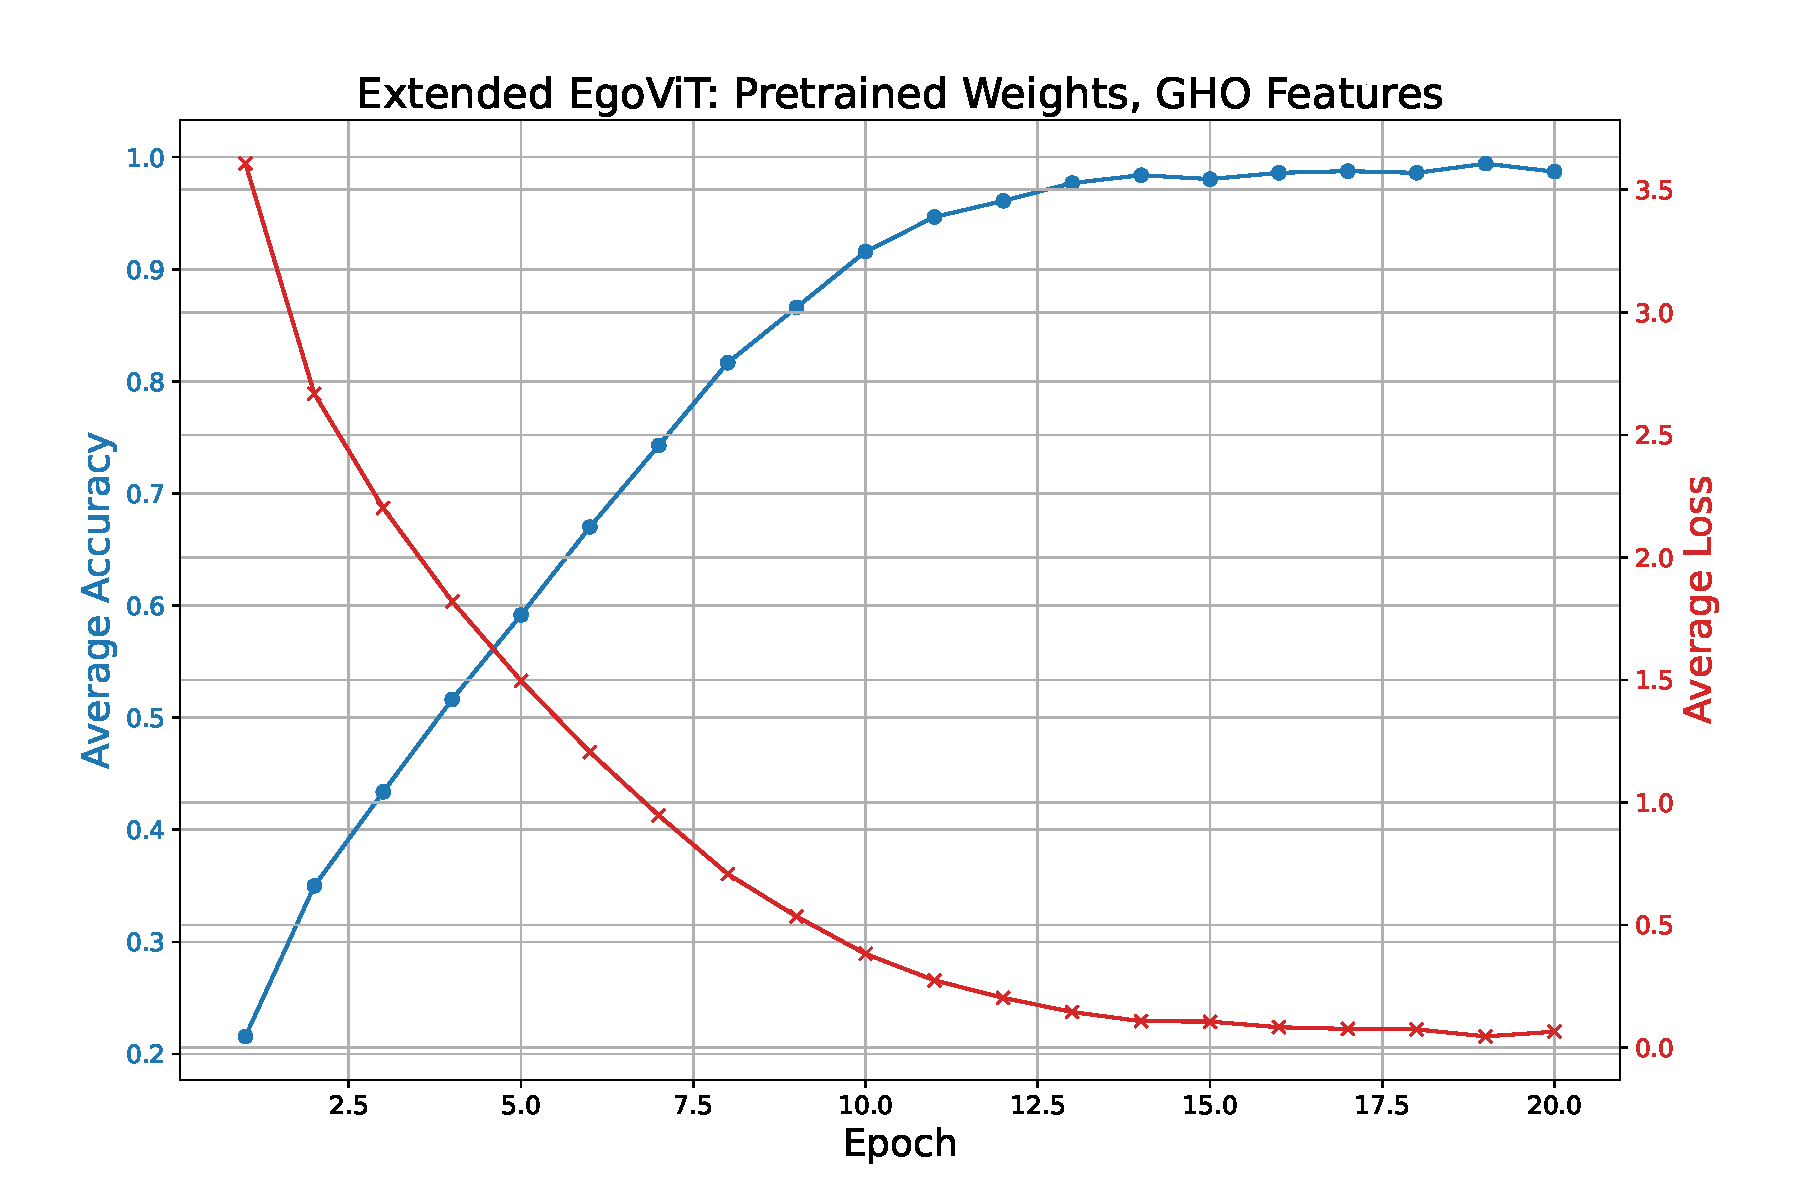
\includegraphics[width=0.9\textwidth]{graphics/figure41}
    \caption{Training loss and accuracy of the enhanced EgoViT with gaze-hand-object features. Blue curve: training accuracy, red curve: training loss.}
    \label{fig:egovit-with-gho}
\end{figure}
\begin{figure}
    \centering
    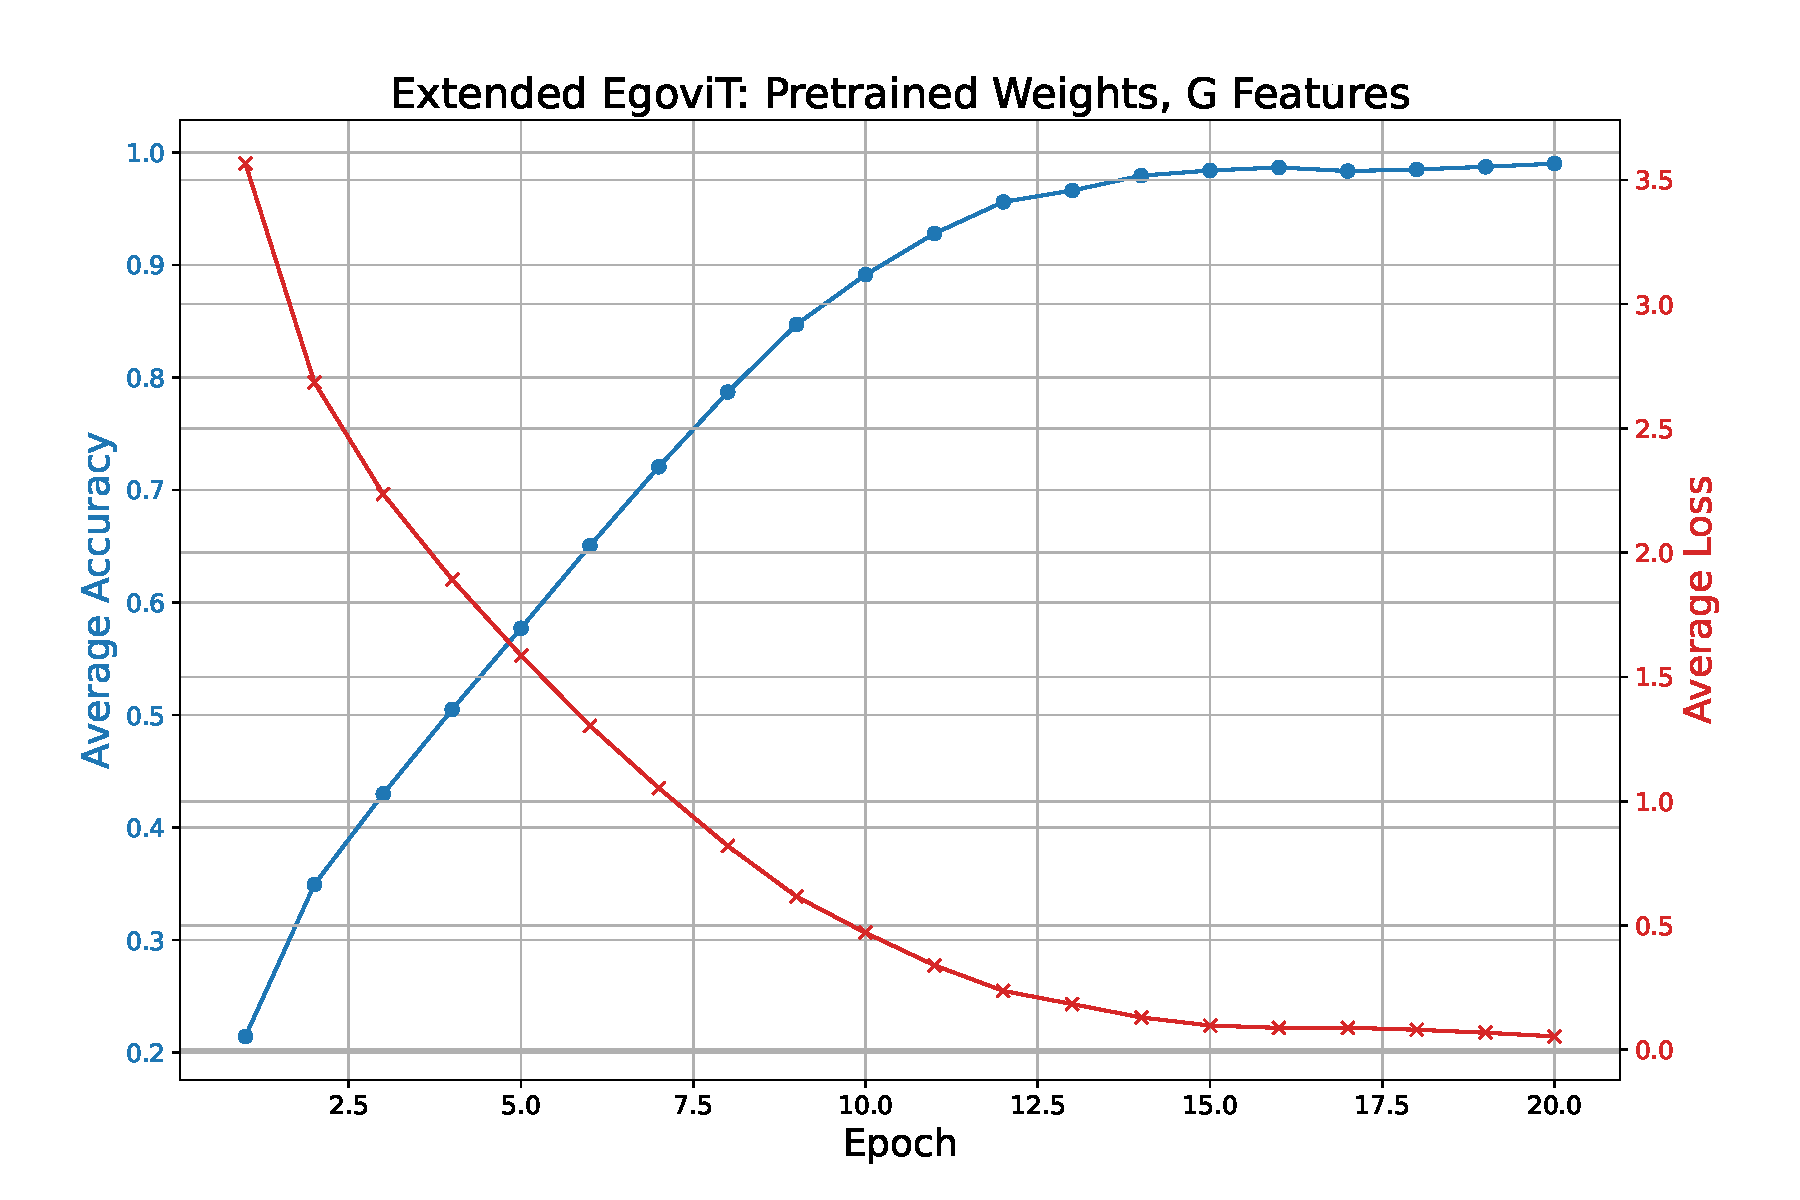
\includegraphics[width=0.9\textwidth]{graphics/figure51}
    \caption{Training loss and accuracy of the enhanced EgoViT with gaze features. Blue curve: training accuracy, red curve: training loss.}
    \label{fig:egovit-with-gaze}
\end{figure}
\newpage
\begin{figure}[htbp]
    \centering
    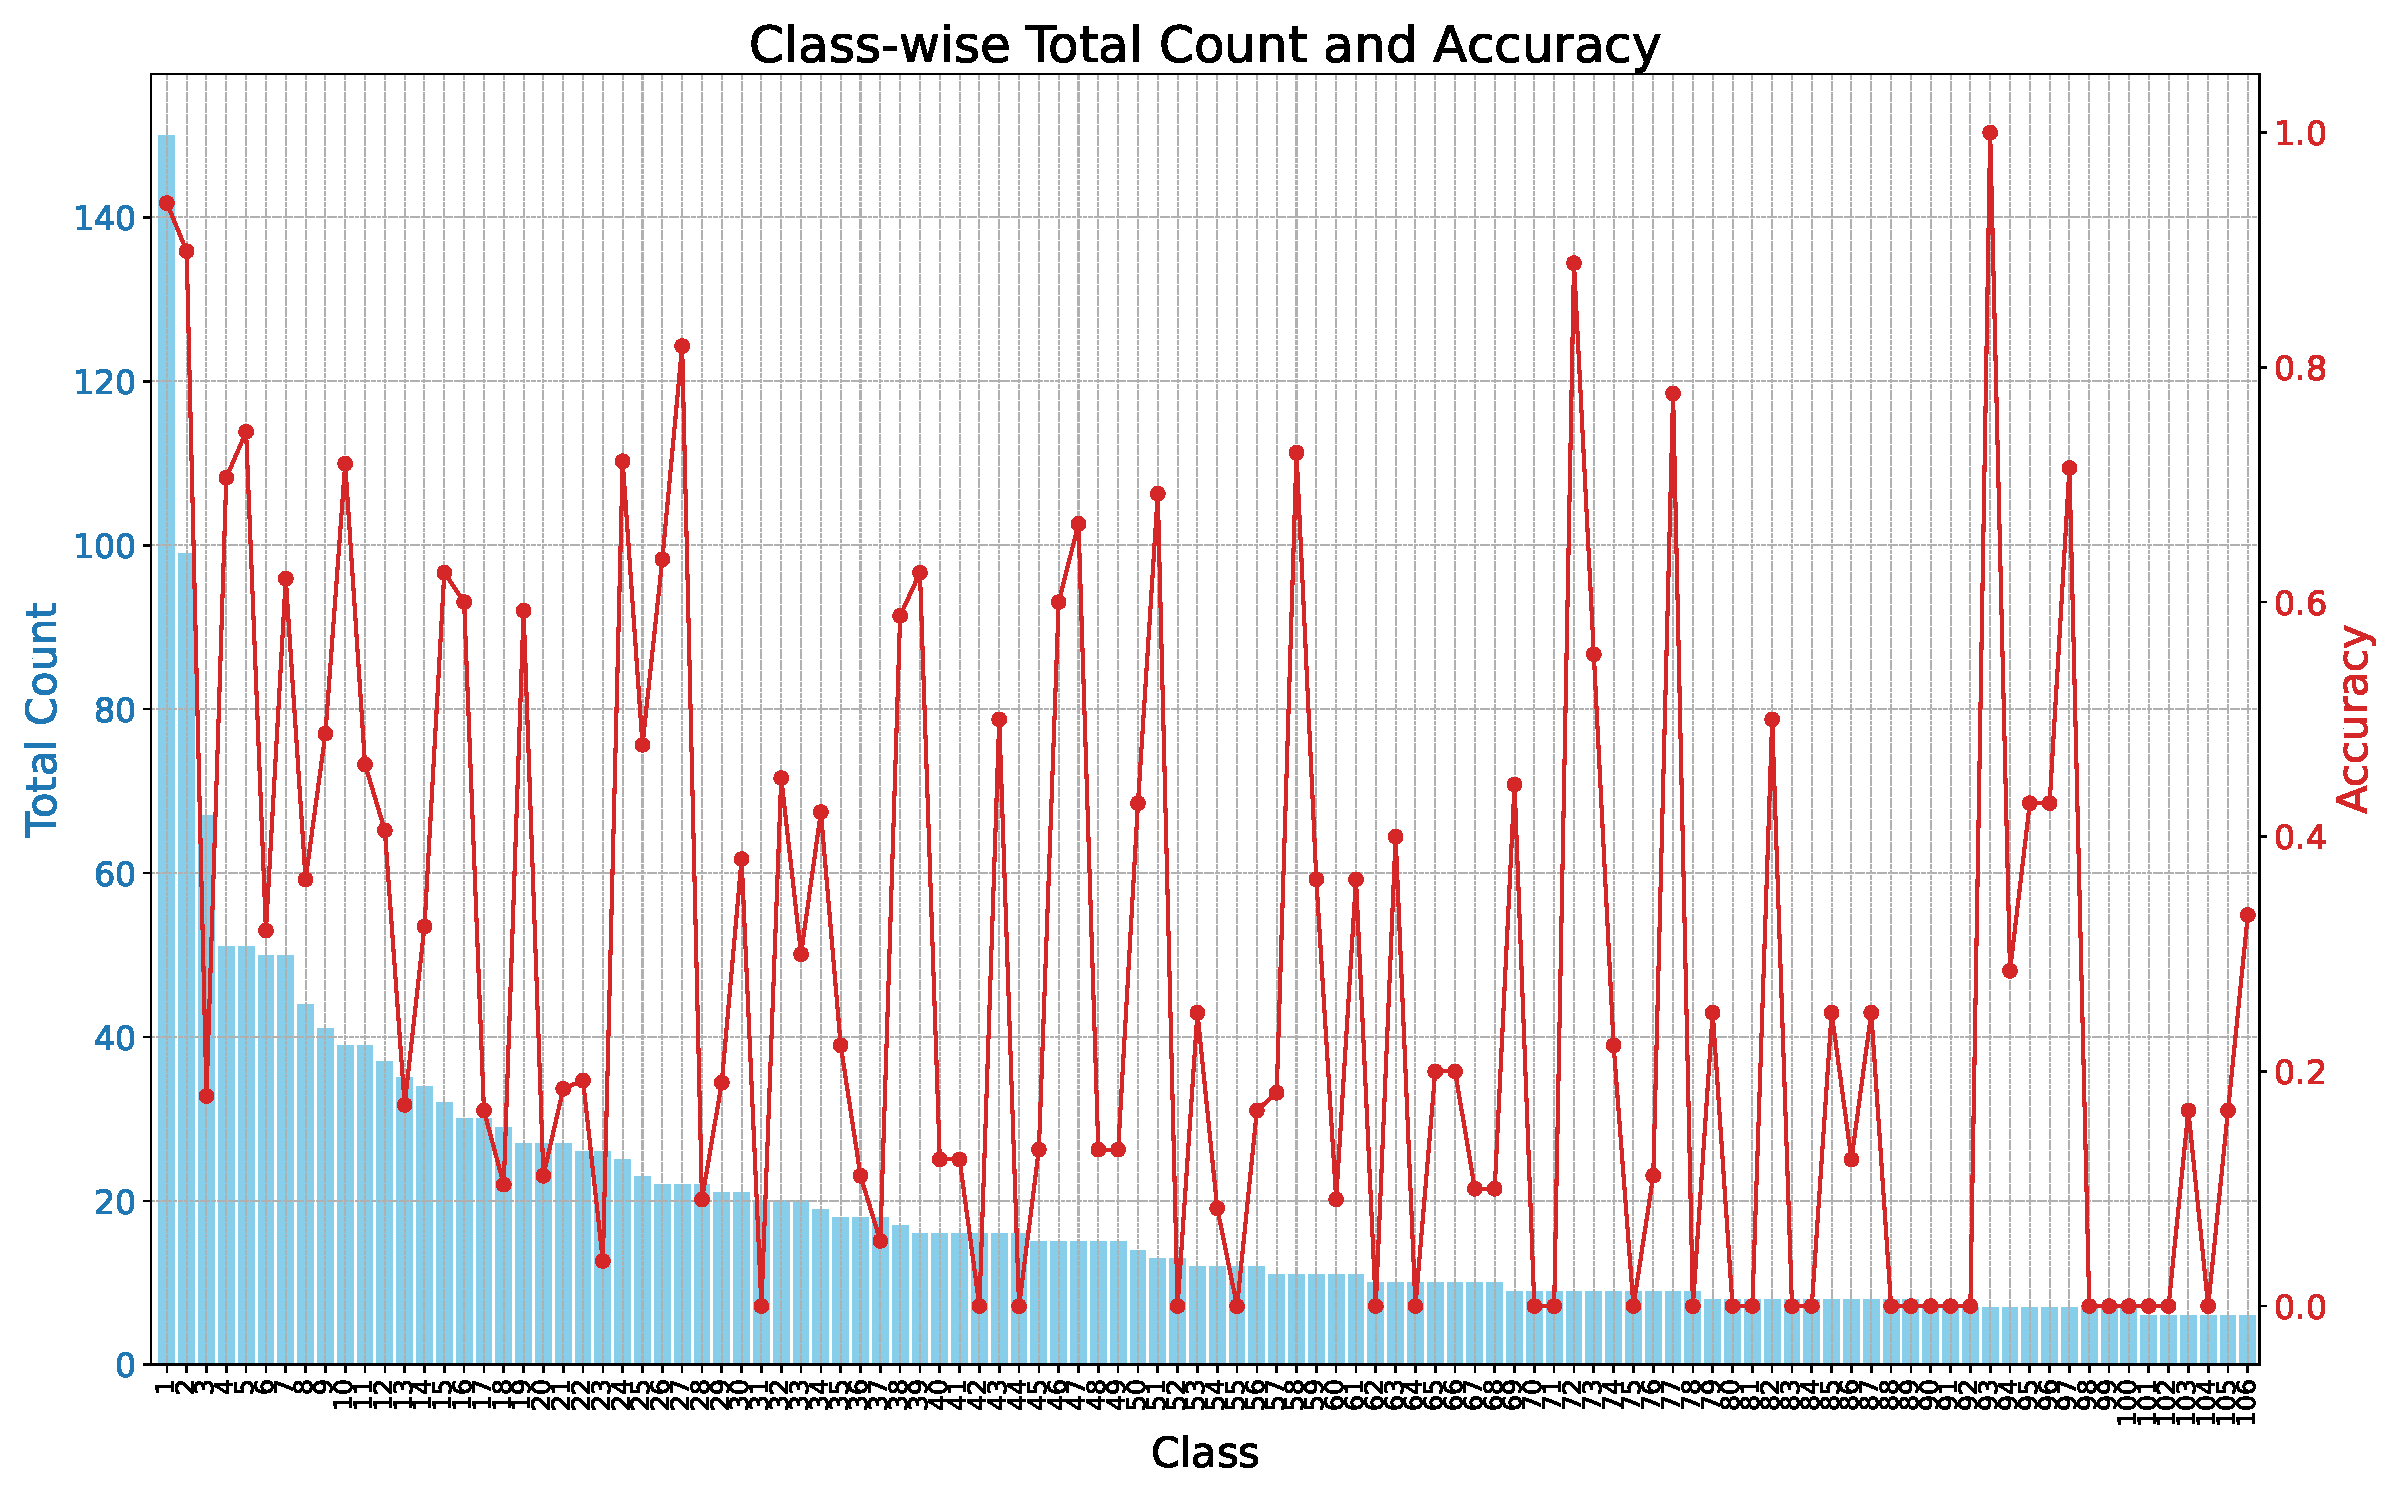
\includegraphics[width=\textwidth]{graphics/2in1}
    \caption{The class-wise total count (blue bars) and accuracy (red line) of the enhanced EgoViT model. The x-axis represents the different classes, while the left y-axis shows the total count of instances per class, and the right y-axis shows the accuracy for each class. }
    \label{fig:action_class}
\end{figure}
\vspace{3mm}
The number of samples for each action class (a total of 106 classes) in the test split1 is calculated and shown in Figure \ref{fig:action_class}. The x-axis represents the action class, and the y-axis represents the number of samples in each class. The top-1 accuracy of the model with gaze-hand-object features is indicated by the red line in Figure \ref{fig:action_class}. This figure shows the number of samples for each action class and the corresponding accuracy of the model with gaze-hand-object features. Class label 1 has the highest number of samples at 150, while the other classes have significantly fewer samples. From class label 31 to 106, the number of samples is under 20. The accuracy of action recognition for many classes with fewer samples is low, with some classes having an accuracy of 0. Since the distribution of samples in each class in train split1 is similar to that in test split1, the model is not able to effectively learn the features of classes with fewer samples.

Two experiments are conducted to explore the effect of gaze quality on the model. The enhanced EgoViT is trained with gaze-hand-object features and only gaze features, using gaze data extracted from gaze version 2. The hyperparameters for training remain the same as in the previous experiments. Table \ref{tab:Results_table3} shows the results and compares them with the results of the experiments Enh\_GHO and Enh\_G. The top-1 accuracy indicates that the model trained with gaze version 2 performs better than the model trained with gaze version 1.
The experiment Enh\_GHO\_v2 achieves a top-1 accuracy of 0.520, which is 0.6\% higher than the experiment Enh\_GHO. The experiment Enh\_G\_v2 achieves a top-1 accuracy of 0.500, which is 1.1\% higher than the experiment Enh\_G and top-5 accuracy also improves by about 1.1\%. These results demonstrate that the quality of gaze features significantly affects the model's performance. This effect is more noticeable when only gaze information is used.
\vspace{5mm}
\begin{table}[htbp]
    \centering
    \caption{Test Results on Gaze Version 1 and Gaze Version 2}
    \begin{tabular}{lccc}
    \hline\hline
    Experiment ID & Top-1 Acc.(\%)& Top-5 Acc.(\%)& Mean Class Acc.(\%) \\
    \hline
    Enh\_GHO     & 51.4 & 76.7 & 40.0 \\
    Enh\_G       & 48.9 & 75.1 & 37.7 \\
    Enh\_GHO\_v2 & 52.0 & 76.3 & 38.7 \\
    Enh\_G\_v2   & 50.0 & 76.2 & 38.0 \\
    \hline\hline
    \end{tabular}
    \label{tab:Results_table3}
\end{table}


\section{Training Variants of the Enhanced EgoViT}
\label{sec:Training Variants of the Extended EgoViT}
In this section, two variants of the enhanced EgoViT model are trained and evaluated. The first variant, referred to as enhanced EgoViT version 2, has a modified \gls{dctg} and \gls{padm} module. The second variant, referred to as enhanced EgoViT version 3, has a modified head. Both variants are trained with the same hyperparameters as the previous experiments, and gaze version 2 is utilized.

The \gls{dctg} module of enhanced EgoViT version 2 features a different feature merging mechanism.  The gaze features and hand-object features are concatenated, and average pooling is not applied to the concatenated features. Thus, the output, i.e., the class token, has a shape of [32, 2, 2048]. This means that the gaze features and hand-object features are not merged into a single feature but are kept separate and processed independently in subsequent layers. In the \gls{padm} module, only the gaze features from the $G$ groups are merged. At the end, only the gaze features are used as the class token for classification, while the hand-object features are included in the information exchange in the Video Swin Transformer.\newpage

\begin{figure}[htbp]
    \centering
    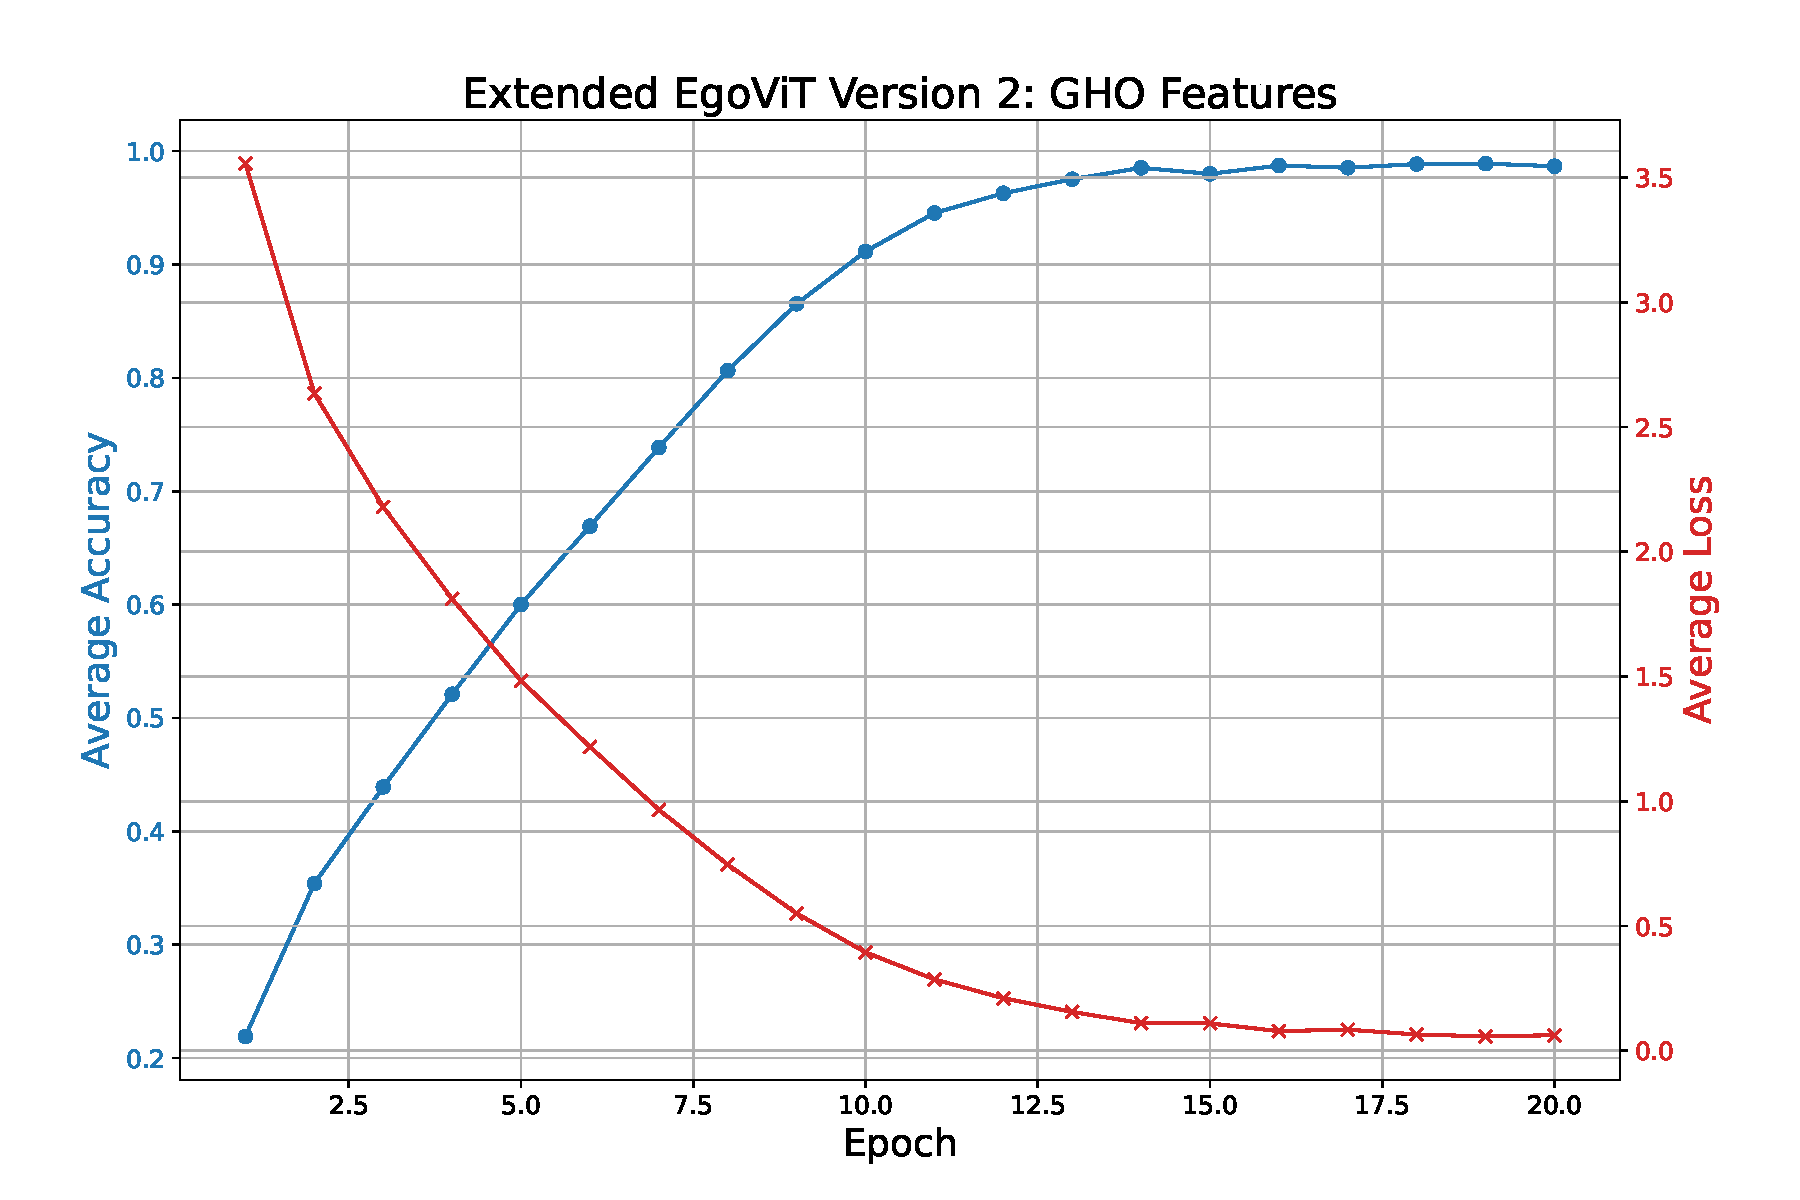
\includegraphics[width=0.9\textwidth]{graphics/figure6}
    \caption{Training loss and accuracy of the enhanced EgoViT version 2 with gaze-hand-object features. Blue curve: training accuracy, red curve: training loss.}
    \label{fig:egovit_v2_GHO}
\end{figure}
\vspace{3mm}
The training loss and accuracy of the enhanced EgoViT version 2 with gaze-hand-object features are shown in Figure \ref{fig:egovit_v2_GHO}. Comparing with Figure \ref{fig:egovit-with-gho} the loss and accuracy curves of the two experiments are similar. They both reach the minimum loss after 15 epochs and have the kinks points at epoch 2 and 15. This training result indicates that the gaze features and hand-object features can be used as class tokens in the model and processed independently. This modification does not significantly affect the model's training performance.

The testing results of the enhanced EgoViT version 2 with gaze-hand-object features are shown in Table \ref{tab:Results_table4}. The model achieves a top-1 accuracy of 50.2\%, a top-5 accuracy of 75.8\%, and a mean class accuracy of 38.3\%. These results are lower than those of the experiment Enh\_GHO\_v2. This indicates that the modified \gls{dctg} and \gls{padm} modules do not improve the model's performance. 
\vspace{5mm}
\begin{table}[htbp]
    % \mycaption{Comparison of Test Results on EgoViT with gaze information}{ddd}
    \centering
    \caption{Comparison of Test Results on EgoViT with Gaze Information}
    \begin{tabular}{lccc}
    \hline\hline
    Training Method & Top-1 Acc.(\%)& Top-5 Acc.(\%)& Mean Class Acc.(\%) \\
    \hline
    Enh\_GHO\_v2 & 52.0 & 76.3 & 38.7 \\
    Enh\_v2\_GHO\_v2 & 50.4 & 75.8 & 38.3 \\
    \hline\hline
    \end{tabular}
    \label{tab:Results_table4}
\end{table}
\clearpage
The second variant, enhanced EgoViT version 3, has a different input configuration for the head. Both the weighted class token and the normal token from the long-term stage are directly fed into the head without separation. To evaluate the effect of this input configuration, the variant enhanced EgoViT version 3 is trained with hand-object features, gaze features, and gaze-hand-object features. The training loss and accuracy of the enhanced EgoViT version 3 with hand-object features, gaze-hand-object features, and only gaze features are shown in Figure \ref{fig:egovit_v3_HO}, \ref{fig:egovit_v3_GHO}, and \ref{fig:egovit_v3_G} respectively. They exhibit similar loss convergence curves, reaching the minimum loss after 15 epochs. 

Additionally, the training loss of experiments Enh\_GHO,  Enh\_GHO\_v2, and \\ Enh\_GHO\_v3 are compared in Figure \ref{fig:loss_comparison}. The loss curves of Enh\_GHO and Enh\_GHO\_v2 represented by lines with cross markers and lines with circle markers, exhibit a similar curve trend. The line with square markers represents Enh\_GHO\_v3, which converges more slowly between epochs 4 and 15. This result indicates that the input configuration of the head and independently processing gaze features and hand-object features in the short-term and long-term stages do not significantly affect the model's training performance.

\begin{figure}[htbp]
    \centering
    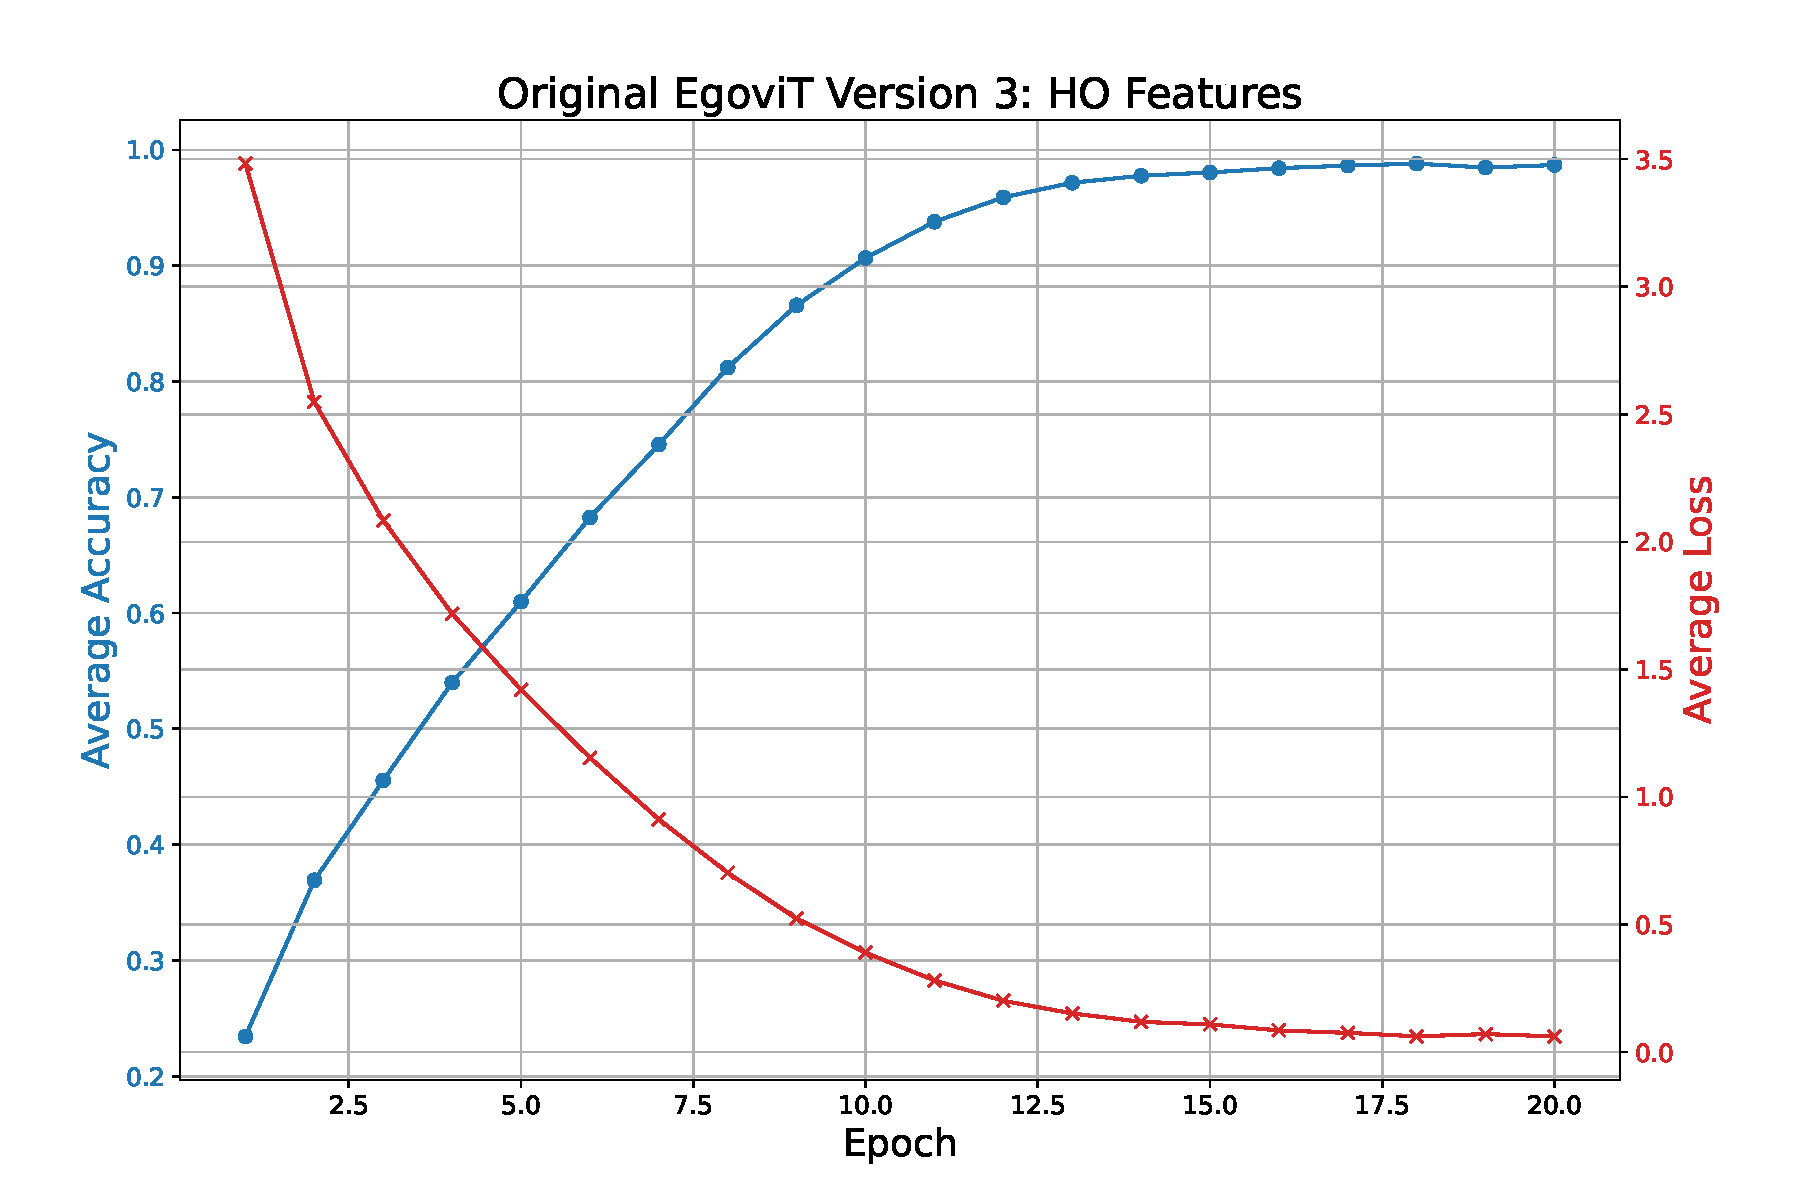
\includegraphics[width=0.9\textwidth]{graphics/figure7}
    \caption{Training loss and accuracy of the original EgoViT version 3 with hand-object features. Blue curve: training accuracy, red curve: training loss.}
    \label{fig:egovit_v3_HO}
\end{figure}
\clearpage
\begin{figure}
    \centering
    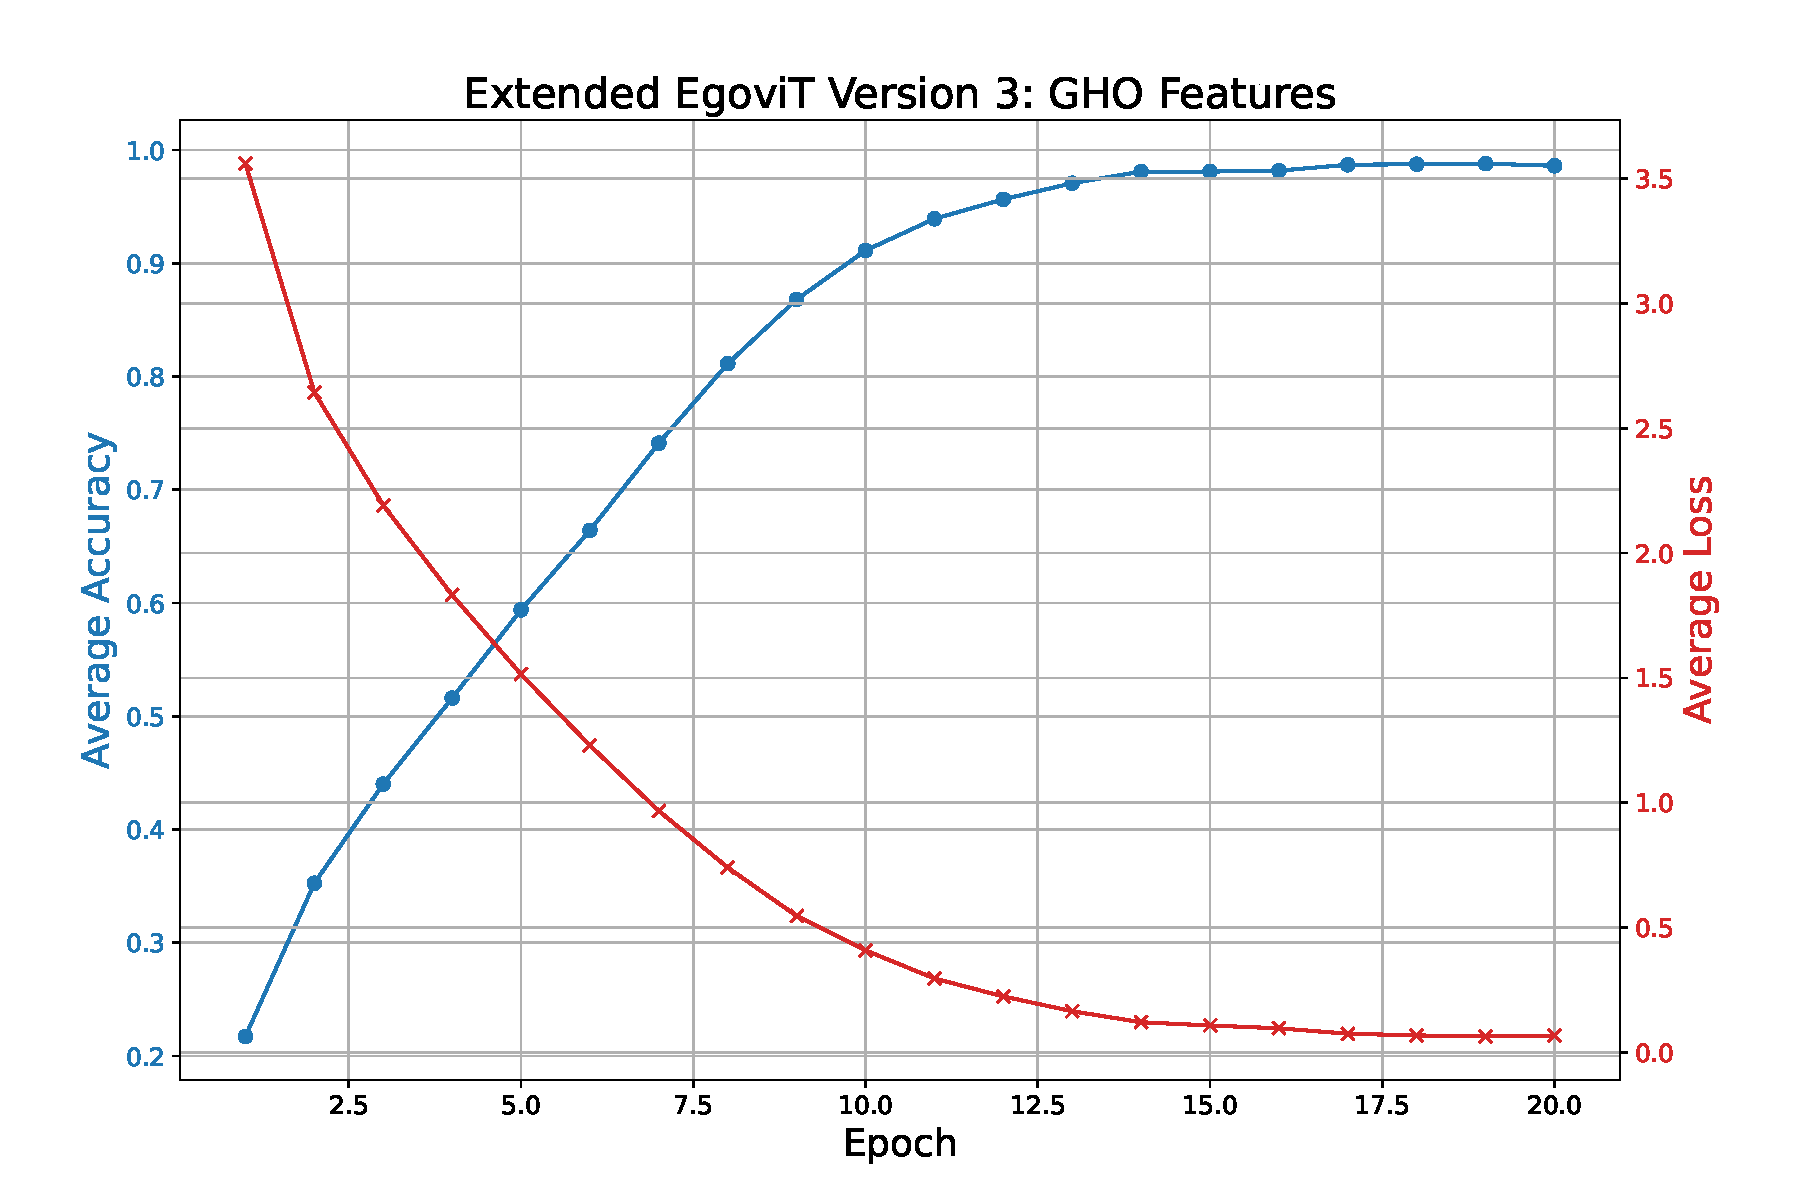
\includegraphics[width=0.9\textwidth]{graphics/figure8}
    \caption{Training loss and accuracy of the enhanced EgoViT version 3 with gaze-hand-object features. Blue curve: training accuracy, red curve: training loss.}
    \label{fig:egovit_v3_GHO}
\end{figure}
\begin{figure}
    \centering
    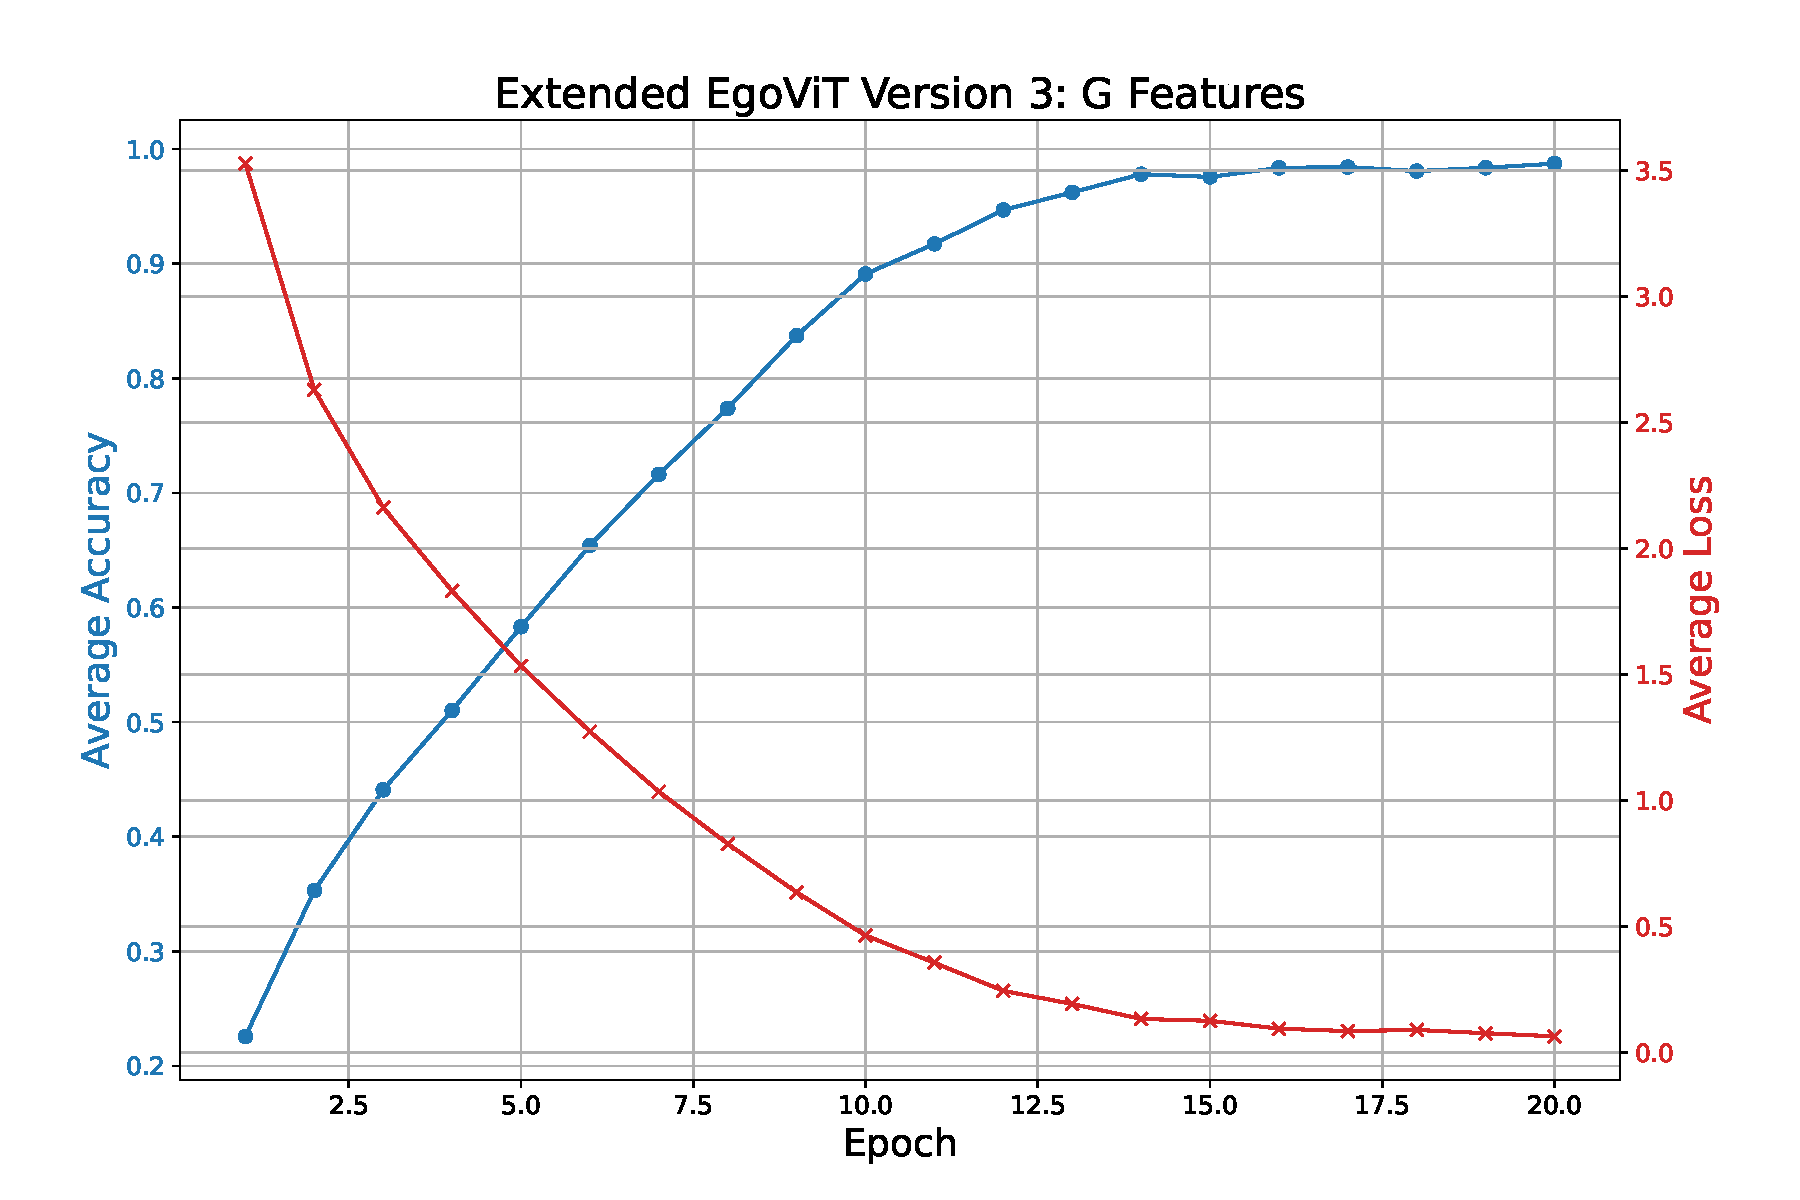
\includegraphics[width=0.9\textwidth]{graphics/figure9}
    \caption{Training loss and accuracy of the enhanced EgoViT version 3 with gaze features. Blue curve: training accuracy, red curve: training loss.}
    \label{fig:egovit_v3_G}
\end{figure}
\clearpage
\begin{figure}[htbp]
    \centering
    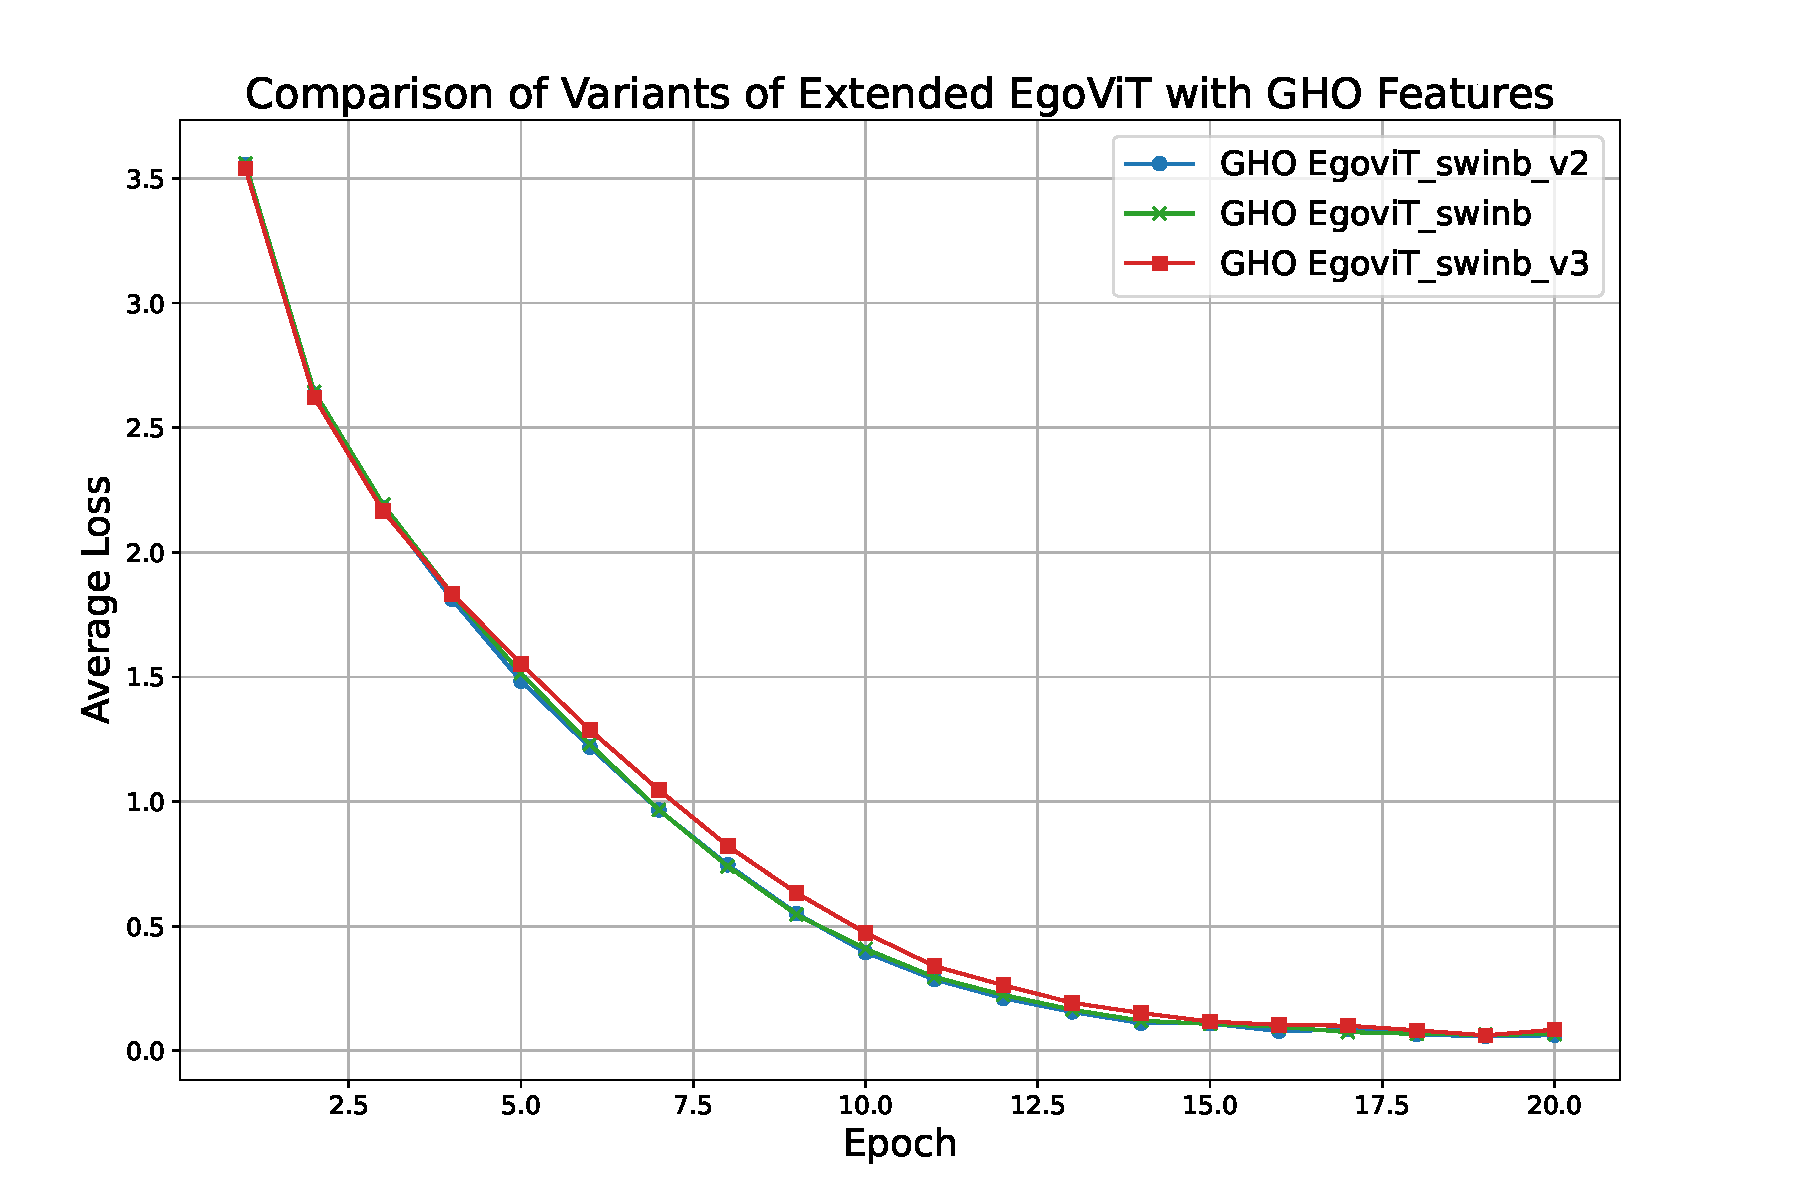
\includegraphics[width=0.9\textwidth]{graphics/loss}
    \caption{Comparison of training loss of the variants of enhanced EgoViT with gaze-hand-object features.}
    \label{fig:loss_comparison}
\end{figure}
% \vspace{5mm}
\begin{table}[htbp]
    \centering
    \caption{Test Results on EgoViT Version 3 Trained on Different Features}
    \begin{tabular}{lccc}
    \hline\hline
    Experiment ID & Top-1 Acc.(\%)& Top-5 Acc.(\%)& Mean Class Acc.(\%) \\
    \hline
    Orig\_v3\_HO & 51.1 & 77.4 & 40.5 \\
    Enh\_v3\_GHO\_v2 & 51.2 & 77.9 & 39.2 \\
    Enh\_v3\_G\_v2   & 50.8 & 75.9 & 37.8 \\
    \hline\hline
    \end{tabular}
    \label{tab:Results_table5}
\end{table}
\vspace{5mm}
The testing results of the enhanced EgoViT version 3 with hand-object features, gaze-hand-object features, and only gaze features are shown in Table \ref{tab:Results_table5}. The experiment orig\_v3\_GHO achieves the highest top-1 and top-5 accuracy of 51.2\% and 77.9\%, respectively. However, However, the results are almost the same as those of the experimen Orig\_v3\_HO, with only 0.1\% and 0.5\% higher top-1 and top-5 accuracy, respectively. The experiment Enh\_v3\_G\_v2 achieves the loswest accuracy across all three metrics. This result indicates that the input configuration of the head does not significantly affect the \gls{ear} performance.

\section{Disscussion}
\label{sec:Disscussion}
The results of all experiments are analyzed and discussed in this section. A comparison of the three metrics (top-1 accuracy, top-5 accuracy, and mean class accuracy) for all experiments is shown in Table \ref{tab:Results_all}, providing an overview of the inference results.

The experiments conducted in section \ref{sec:training_original_egovit} show that the original EgoViT performs better with pretrained weights from the Video Swin Transformer. Although the pretrained weights are trained on an image dataset and the architecture of the Video Swin Transformer is modified, the model with a fixed learning rate of $1 \mathrm{e}{-5}$ achieves better accuracy than the model with a scheduler learning rate as followed by \cite{liu_video_2021}. The configuration of the learning rate for different layers in the model has the potential to affect model accuracy, thus a new configuration could be explored in future work.

In experiments Enh\_GHO, Enh\_G, Enh\_GHO\_v2, and Enh\_G\_v2, two versions of gaze data are used for training. The results show that the model trained with gaze version 2 performs better than the model trained with gaze version 1. The quality of collected gaze tracking data significantly affects the model's performance, especially when only gaze information is used. The two additional experiments on the variants of the enhanced EgoViT show that the modified \gls{dctg} and \gls{padm} modules, as well as the input configuration of the head, do not improve the model's performance. One reason could be that the information in the class token, i.e., the gaze and hand-object features, are already exchanged with the normal token in the 3D Shifted \gls{msa} in the Video Swin Transformer. Therefore, even the gaze and hand-object features are processed independently in the short-term and long-term stages, the class token has the surfficient information for classification.

A noticeable obeservation is all experiments have a mean accuracy under 41\%, and the top-1 accuracy is only around 50\%. The sesults achieves lower performance than the Video Swin Transformer trained on other datasets. A plausible reason for this is that the EGTEA Gaze+ dataset is more challenging than other datasets. This dataset has an imbalanced distribution of samples in each class, with some classes having fewer than 40 samples. While class label 1 has about 600 samples. The model may not able to effectively learn the features of classes with fewer samples. 
\newpage
Although the dataset is challenging, the results of the experiment Enh\_GHO\_v2 shows a promising improvement in the performance of \gls{ear}. The enhanced EgoViT model trained with gaze-hand-object features achieves a top-1 accuracy of 52.0\% and a top-5 accuracy of 76.3\%. These results are higher than those of the original EgoViT model trained with hand-object features. This demonstrates that integrating additional gaze information can potentially improve \gls{ear} performance. The work in this thesis provides a foundation for future research on the use of gaze information in \gls{ear}.


\vspace{5mm}
\begin{table}[htbp]
    \centering
    \caption{Test Results of Various Experiments}
    \begin{tabular}{lccc}
    \hline\hline
    Experiment ID & Top-1 Acc.(\%)& Top-5 Acc.(\%)& Mean Class Acc.(\%) \\
    \hline
    Orig\_HO\_no\_pretrain & 51.5 & 78.5 & 38.8 \\
    Orig\_HO               & 51.7 & 75.2 & 40.6 \\
    Orig\_HO\_sched. LR    & 48.4 & 74.4 & 35.8 \\
    Enh\_ GHO           & 51.4 & 76.7 & 40.0 \\
    Enh\_G              & 48.9 & 75.1 & 37.7 \\
    Enh\_GHO\_v2        & 52.0 & 76.3 & 38.7 \\
    Enh\_G\_v2          & 50.0 & 76.2 & 38.0 \\
    Enh\_v2\_GHO\_v2    & 50.4 & 75.8 & 38.3 \\
    Enh\_v3\_HO         & 51.1 & 77.4 & 40.5 \\
    Enh\_v3\_GHO\_v2    & 51.2 & 77.9 & 39.2 \\
    Enh\_ v3\_G\_v2     & 50.8 & 75.9 & 37.8 \\
    \hline\hline
    \end{tabular}
    \label{tab:Results_all}
\end{table}
\chapter{Summary}
\label{chap:summary}

\section{Conclusion}
\label{sec:conclusion}
In this thesis, a Gaze-Enhanced \gls{dctg} module for the EgoViT model was proposed to improve action recognition performance in egocentric videos. The Gaze-Enhanced \gls{dctg} is designed to focus on additional regions of interest in the video frames, identified by gaze tracking points and detected hands and objects. Compared to the original EgoViT, the proposed Gaze-Enhanced EgoViT incorporates gaze tracking points as an additional input to the model. The Gaze-Enhanced \gls{dctg} module extracts gaze features from the gaze tracking points and input frames, merging them with hand-object features from a modified \gls{hod} module to generate dynamic class tokens. These dynamic class tokens guide the model to focus on regions enriched with gaze and hand-object information.

The proposed Gaze-Enhanced EgoViT model retains a similar architecture to the original EgoViT model, consisting of $G$ groups in the short-term stage, a class token Merging module, and a long-term stage. This architecture effectively handles temporal relationships between short-term phases. To process local relationships along the spatial dimension, a modified Video Swin Transformer is used as the backbone of the proposed model.

The proposed Gaze-Enhanced EgoViT model was evaluated on the EGTEA Gaze+ dataset, a comprehensive dataset for first-person view actions with gaze tracking points. The experimental results demonstrate that the proposed Gaze-Enhanced EgoViT model achieves a top-1 accuracy of 52.0\% and a top-5 accuracy of 76.3\%, representing an improvement over the baseline EgoViT model. The model was trained and tested on two versions of gaze data. Gaze version 2, with better gaze feature quality, yielded better performance, suggesting that the quality of gaze features significantly impacts the model's performance. Those results suggest that the quality of gaze features plays a significant role in the model's performance. The proposed Gaze-Enhanced EgoViT model is a promising approach to improving action recognition in egocentric videos. Additionally, experiments conducted on the model with only gaze features showed that it achieves a top-1 accuracy above 50\%, indicating that gaze information is useful for action recognition in egocentric videos. Further investigation into the impact of gaze information on \gls{ear} is warranted. 

\section{Future Works and Outlook}
\label{sec:future_work}
\textbf{Futere work:} The experimental results indicate that the proposed Gaze-Enhanced EgoViT model is a promising approach for improving action recognition performance in egocentric videos. To significantly enhance the model's performance, improving the quality of gaze features should be explored. There are three possibilities for this:
\begin{enumerate}
    \item Training and evaluating the model on a dataset with more accurate collected gaze tracking points.
    \item Studying the impact of gaze region size on \gls{ear}. Conducte experiments with different gaze-box sizes to determine the optimal size for the model.
    \item Using pretrained networks, such as autoencoders, to extract gaze features. An autoencoder can be trained to extract features from images and reconstruct the images, accuiring higher quality extracted features.
\end{enumerate}

\textbf{Outlook in the field of battery production:} The rapid growth of electric vehicles has increased the demand for batteries, making their production a key technology for value creation. As the demand and production of electric vehicles rise, so does the need for high-quality batteries. Gigafactories are being built to meet this demand, optimizing production quality, performance, and cost. Artificial intelligence technologies, such as computer vision and machine learning, are increasingly used in battery production to enhance quality. Niri et al. \cite{niri2021machine} combined machine learning to create predictive models for battery performance, linking lab-scale manufacturing to pilot-line production and supporting smarter and cleaner electrode production for high-quality Li-ion batteries. Smart factories are equipped with many industrial robotic arms, and ensuring the safety of interactions between workers and robotic arms is crucial. Suh et al. \cite{suh2023workeractivityrecognitionmanufacturing} presented a novel wearable sensing prototype integrating IMU and body capacitance sensors to recognize worker activities in manufacturing.

These studies show that artificial intelligence technologies have broad prospects in battery production. The proposed Gaze-Enhanced EgoViT model has the potential to be applied in various ways to improve production quality. For example, it could be used to monitor robotic arm activities to ensure process accuracy and avoid collisions with workers. Since the model can handle egocentric videos, the monitoring camera could be directly mounted on the moving part of the robotic arm, providing a first-person view and enhancing the environmental perception of the robotic arm. Another application could be wearable equipment for workers, such as glasses with cameras and gaze tracking functions. The proposed Gaze-Enhanced EgoViT model can recognize worker activities and identify which part of the production process the worker is engaged in, improving assembly quality by detecting anomalies in real-time. The Transformer-based model is suitable for handling varying sequence video lengths, making it ideal for real-time monitoring of different production processes performed by workers. The model has the potential to understand the relationships between different production processes and provide feedback to workers in real-time, thereby improving production efficiency and quality.
% \include{chapters/latex-tipps}
\phantomsection

% Anhang %%%%%%%%%%%%%%%%%%%%%%%%%%%%%%%%%%%%%%%%
%\begin{appendix}
%\renewcommand{\chaptermark}[1]{\markboth{\MakeUppercase{\appendixname\ \thechapter.\ #1}}{}} % \thechapter=Number of chapter
%Argument #1 is the name of the chapter
% \include{appendix/anhang1}
%\end{appendix}

\renewcommand{\chaptermark}[1]{\markboth{\MakeUppercase{#1}}{}} %\chaptername=Kapitel \thechapter=Nummer %Argument #1 ist der Name des kapitels

%%%%%%%%%%%%%%%%%%%%%%%%%%%%%%%%%%%%%%%%%%%%%%%%%%%%%%%%
% Abkürzungsverzeichnis
\clearpage % bei Option "oneside"
%\cleardoublepage % bei Option "twoside"
% \newpage
\renewcommand{\glossaryname}{List of Abbreviations}
% \chapter*{\glossaryname} %\nomname
\addcontentsline{toc}{chapter}{\acronymname}
% \addcontentsline{toc}{chapter}{List of Abbreviations}
\markboth{\MakeUppercase{\acronymname}}{\acronymname}
% \printnoidxglossaries
\printnoidxglossaries
% \printglossary[type=\acronymtype]
% \markboth{\MakeUppercase{\nomname}}{\nomname}
%\printnomenclature[2cm]
% Print the glossary
%\cleardoublepage % bei Option "twoside"
% 
\newacronym{abc}{ABC}{A Basic Concept}
\newacronym{er}{ER}{error rate}
\newacronym{fr}{FR}{Fehlerrate}
\newacronym[plural={RDBMS},shortplural={RDBMS}]{rdbms}{RDBMS}{Relational Database Management System}
\newacronym{vr}{VR}{Virtual Reality}
\newacronym{hri}{HRI}{Human-Robot Interaction}
\newacronym{ear}{EAR}{egocentric action recognition}
\newacronym{vit}{ViT}{Vision Transformer}
\newacronym{dctg}{DCTG}{dynamic class token generator}
\newacronym{padm}{PADM}{Pyramid Architecture with a Dynamic Merging}
\newacronym{fpv}{FPV}{first person view}
\newacronym{hod}{HOD}{Hand and Object Detector}
\newacronym{cnn}{CNNs}{convolutional neural networks}
\newacronym{tsn}{TSN}{Temporal Segment Networks}
\newacronym{tsm}{TSM}{termed temporal shift module}
\newacronym{nlp}{NLP}{natural language processing}
\newacronym{vivit}{ViViT}{Video Vision Transformer}
\newacronym{vst}{}{Video Swin Transformer}
\newacronym{msa}{MSA}{multi-Head Self-Attention}
\newacronym{ffn}{FFN}{feed-forward network}
\newacronym{ln}{LN}{Layer Normalization}
\newacronym{dct}{DCT}{Dynamic Class Token}
\newacronym{gedctg}{GEDCTG}{Gaze-Enhanced Dynamic Class Token Generator}
\newacronym{lstm}{LSTM}{long short-term memory}
% \addcontentsline{toc}{chapter}{Abbreviations}
% \markboth{\MakeUppercase{Abbreviations}}{List of Abbreviations}
% \printglossary[type=\acronymtype, title=List of Abbreviations]
%%%%%%%%%%%%%%%%%%%%%%%%%%%%%%%%%%%%%%%%%%%%%%%%%%%%%%%%
% List of Tables
%\cleardoublepage
\renewcommand{\listtablename}{List of Tables}
\addcontentsline{toc}{chapter}{List of Tables}
\listoftables
%\markboth{List of Tables}{List of Tables}
%

%%%%%%%%%%%%%%%%%%%%%%%%%%%%%%%%%%%%%%%%%%%%%%%%%%%%%%%%
% List of Figures
%\cleardoublepage
\renewcommand{\listfigurename}{List of Figures}
\addcontentsline{toc}{chapter}{List of Figures}
\listoffigures
%%\markboth{List of Figures}{List of Figures}
%\cleardoublepage

%%%%%%%%%%%%%%%%%%%%%%%%%%%%%%%%%%%%%%%%%%%%%%%%%%%%%%
% Sticwortverzeichnis
% \renewcommand{\indexname}{Stichwortverzeichnis}
% \addcontentsline{toc}{chapter}{Stichwortverzeichnis}
% \printindex


%%%%%%%%%%%%%%%%%%%%%%%%%%%%%%%%%%%%%%%%%
%bibliography
%%%%%%%%%%%%%%%%%%%%%%%%%%%%%%%%%%%%%%%%%
\renewcommand{\bibname}{Bibliography}
\newpage
\phantomsection
\addcontentsline{toc}{chapter}{Bibliography}
\printbibliography

%use Danksagung as template!
% \include{chapters/Danksagung}

%%%%%%%%%%%%%%%%%%%%%%%%%%%%%%%%%%%%%%%
%\end{myenvironment}
\end{document}
